%
% NOTES:  
%  - Be sure to place captions BEFORE labels in figures and tables!
%    Otherwise, numbering will be incorrect.  For example, use the following:
%       \caption{PETSc Vector Operations}
%       \label{fig_vectorops}
%  - Use \break to indicate a line break (needed to prevent long strings in
%    \tt mode from running of the page)
%

\cleardoublepage
\chapter{Vectors and Distributing Parallel Data} 
\label{chapter_vectors}
\sindex{vectors}

The vector (denoted by Vec) is one of the simplest PETSc
objects.  Vectors are used to store discrete PDE solutions, right-hand
sides for linear systems, etc. This chapter is organized as follows:

\begin{itemize}
\item (Vec) Sections~\ref{sec_veccreate} and \ref{sec_vecbasic} - basic usage of vectors
\item Section \ref{sec_indexingandordering} - management of the various numberings of
               degrees of freedom, vertices, cells, etc.
  \begin{itemize} 
  \item (AO) Mapping between different global numberings
  \item (ISLocalToGlobalMapping) Mapping between local and global numberings
  \end{itemize}
\item (DA) Section \ref{sec_struct} - management of structured grids
\item (IS, VecScatter) Section \ref{sec_unstruct} - management of vectors related to 
      unstructured grids
\end{itemize}

% --------------------------------------------------------------------------------------
\section{Creating and Assembling Vectors}
\label{sec_veccreate}

PETSc currently provides two basic vector types: sequential and parallel
(MPI based). To create a sequential vector with \trl{m} components,
one can
use the command \findex{VecCreateSeq()} \findex{Vec}
\begin{tabbing}
  VecCreateSeq(PETSC\_COMM\_SELF,int m,Vec *x);
\end{tabbing}
To create a parallel vector one can either specify the number of 
components that will be stored on each process or let PETSc decide. 
The command \findex{VecCreateMPI()}
\begin{tabbing}
  VecCreateMPI(MPI\_Comm comm,int m,int M,Vec *x);
\end{tabbing}
creates a vector that is distributed over all processes in the communicator,
comm, where \trl{m} indicates the number 
of components to store on the local process, and \trl{M} is the 
total number of vector components.  Either the local or global 
dimension, but not both, can be set to PETSC\_DECIDE to 
\findex{PETSC_DECIDE} indicate that PETSc should determine it.
More generally, one can use the routines \findex{VecCreate()} \findex{VecSetSizes()} 
\findex{VecSetFromOptions()}
\begin{tabbing}
  VecCreate(MPI\_Comm comm,Vec *v);\\
  VecSetSizes(Vec v, int m, int M);\\
  VecSetFromOptions(Vec v);
\end{tabbing}
which automatically generates the appropriate vector type 
(sequential or parallel) over all processes in \trl{comm}.
The option \trl{-vec_type} \trl{mpi} can be used in conjunction with 
VecCreate() and VecSetFromOptions() to specify the use of MPI \findex{-vec_type}
vectors even for the uniprocess case.

We emphasize that all processes in \trl{comm} {\em must} call the
vector creation routines, since these routines are collective over all
processes in the communicator. If you are not familar with MPI communicators,
see the discussion in Section \ref{sec_writing} on page \pageref{sec_writing}. 
In addition, if a sequence of \trl{
VecCreateXXX()} routines is used, they must be called in the same
order on each process in the communicator.

One can assign a single value to all components of a vector with the 
command \findex{VecSet()}
\begin{tabbing}
  VecSet(Vec x,PetscScalar value);
\end{tabbing}
Assigning values to individual components of the vector is more 
complicated, in order to make it possible to write efficient parallel 
code.  Assigning a set of components is a two-step process: one 
first calls  \findex{VecSetValues()} \findex{INSERT_VALUES}
\begin{tabbing}
  VecSetValues(Vec x,int n,int *indices,PetscScalar *values,INSERT\_VALUES);
\end{tabbing}
any number of times on any or all of the processes. The argument
\trl{n} gives the number of components being set in this 
insertion. The integer array \trl{indices} contains the {\em global component
indices}, and \trl{values} is the array of values to be inserted.
Any process can set any components of the vector; PETSc insures that 
they are automatically stored in the correct location.
Once all of the values have been inserted with VecSetValues(),
one must call \sindex{assembly}
\begin{tabbing}
  VecAssemblyBegin(Vec x);
\end{tabbing}
followed by \findex{VecAssemblyBegin()}\findex{VecAssemblyEnd()} 
\begin{tabbing}
  VecAssemblyEnd(Vec x);
\end{tabbing}
to perform any needed message passing of nonlocal components.
In order to allow the overlap of communication and calculation,
the user's code can perform any series of other actions between these 
two calls while the messages are in transition. 

Example usage of VecSetValues() may be found in 
\trl{${PETSC_DIR}/src/vec/vec/examples/tutorials/ex2.c} or \trl{ex2f.F}.

Often, rather than inserting elements in a vector, one may wish to 
add values. This process \sindex{vector values, setting}
is also done with the command \findex{VecSetValues()}
\begin{tabbing}
  VecSetValues(Vec x,int n,int *indices, PetscScalar *values,ADD\_VALUES);
\end{tabbing}
Again \findex{ADD_VALUES} one must call the assembly routines 
VecAssemblyBegin() and VecAssemblyEnd() after all of the values
have been added.  Note that addition and insertion calls to 
VecSetValues() {\em cannot} be mixed.  Instead, one must add and insert
vector elements in phases, with intervening calls to the assembly
routines. This phased assembly procedure overcomes the nondeterministic
behavior that
would occur if two different processes generated values
for the same location, with one process adding while the other is inserting
its value.  (In this case the addition and insertion actions could be performed 
in either order,
thus resulting in different values at the particular location. Since
PETSc does not allow the simultaneous use of INSERT\_VALUES and
ADD\_VALUES this nondeterministic behavior will not occur in PETSc.)

You can called VecGetValues() to pull local values from a vector (but
not off-process values),
an alternative method for extracting some components of a vector are
the vector scatter routines.  See Section~\ref{sec_scatter} for details; see also
below for VecGetArray().

One can examine a vector with the command \findex{VecView()}
\begin{tabbing}
  VecView(Vec x,PetscViewer v);
\end{tabbing}
To print the vector to the screen, one can use the viewer
\findex{PETSC_VIEWER_STDOUT_WORLD} \trl{PETSC_VIEWER_STDOUT_WORLD},
which ensures that parallel vectors are printed correctly to
\trl{stdout}. To display the vector in an X-window, one can use the
default X-windows viewer \trl{PETSC_VIEWER_DRAW_WORLD},
\findex{PETSC_VIEWER_DRAW_WORLD} or one can create a viewer with the
routine PetscViewerDrawOpen().  A variety of viewers are discussed
further in Section \ref{sec_viewers}.

To create a new vector of the same format as an existing vector, one uses
the command \findex{VecDuplicate()}
\begin{tabbing}
  VecDuplicate(Vec old,Vec *new);
\end{tabbing}
To create several new vectors of the same format as an existing vector,
one uses the command \findex{VecDuplicateVecs()}
\begin{tabbing}
  VecDuplicateVecs(Vec old,int n,Vec **new);
\end{tabbing}
This routine creates an array of pointers to vectors. The two routines 
are very useful because they allow one to write library code that does 
not depend on the particular format of the vectors being used. Instead,
the subroutines can automatically correctly create work vectors
based on the specified existing vector.  As discussed in 
Section~\ref{sec_fortvecd}, the Fortran interface for VecDuplicateVecs()
differs slightly.

When a vector is no longer needed, it should be destroyed with the 
command \findex{VecDestroy()}
\begin{tabbing}
  VecDestroy(Vec x);
\end{tabbing}
To destroy an array of vectors, use the command \findex{VecDestroyVecs()}
\begin{tabbing}
  VecDestroyVecs(Vec *vecs,int n);
\end{tabbing}
Note that the Fortran interface for VecDestroyVecs() differs slightly,
as described in Section~\ref{sec_fortvecd}.

It is also possible to create vectors that use an array provided by the user, 
rather than having PETSc internally allocate the array space. 
\sindex{providing arrays for vectors}
\sindex{vectors, user-supplied arrays} 
Such vectors can be created with the routines
\begin{tabbing}
  VecCreateSeqWithArray(PETSC\_COMM\_SELF,int n,PetscScalar *array,Vec *V);
\end{tabbing}
and  \findex{VecCreateMPIWithArray()} \findex{VecCreateSeqWithArray()}
\begin{tabbing}
  VecCreateMPIWithArray(MPI\_Comm comm,int n,int N,PetscScalar *array,Vec *vv);
\end{tabbing}
Note that here one must provide the value \trl{n}, it cannot be PETSC\_DECIDE and
the user is responsible for providing enough space in the array; \trl{n*sizeof(PetscScalar)}.


% --------------------------------------------------------------------------------------
\section{Basic Vector Operations}  
\label{sec_vecbasic}
\begin{table}[tb]
\begin{center}
\begin{tabular}{ll}
{\bf Function Name} & {\bf Operation} \\
\hline
VecAXPY(Vec y,PetscScalar a,Vec x); & $ y = y + a*x$ \\
VecAYPX(Vec y,PetscScalar a,Vec x); & $ y = x + a*y$ \\
VecWAXPY(Vec w,PetscScalar a,Vec x,Vec y); & $ w = a*x + y$ \\
VecAXPBY(Vec y,PetscScalar a,PetscScalar b,Vec x); & $ y = a*x + b*y$ \\
VecScale(Vec x, PetscScalar a); & $ x = a*x $ \\
VecDot(Vec x, Vec y, PetscScalar *r); & $ r = \bar{x}'*y$ \\
VecTDot(Vec x, Vec y, PetscScalar *r); & $ r = x'*y$ \\
VecNorm(Vec x,NormType type,  double *r); & $ r = ||x||_{type}$ \\
VecSum(Vec x,   PetscScalar *r); & $ r = \sum x_{i}$ \\
VecCopy(Vec x, Vec y); & $ y = x $ \\
VecSwap(Vec x, Vec y); & $ y = x $ while $ x = y$ \\
VecPointwiseMult(Vec w,Vec x,Vec y); & $ w_{i} = x_{i}*y_{i} $ \\
VecPointwiseDivide(Vec w,Vec x,Vec y); & $ w_{i} = x_{i}/y_{i} $ \\
VecMDot(Vec x,int n,Vec y[],PetscScalar *r); & $ r[i] = \bar{x}'*y[i]$ \\
VecMTDot(Vec x,int n,Vec y[],PetscScalar *r); & $ r[i] = x'*y[i]$ \\
VecMAXPY(Vec y,int n, PetscScalar *a, Vec x[]); \hspace{1cm} & $ y = y + \sum_i a_{i}*x[i] $ \\
VecMax(Vec x,  int *idx, double *r); & $ r = \max x_{i}$ \\
VecMin(Vec x,  int *idx, double *r); & $ r = \min x_{i}$ \\
VecAbs(Vec x); & $ x_i = |x_{i}|$ \\
VecReciprocal(Vec x); & $ x_i = 1/x_{i}$ \\
VecShift(Vec x,PetscScalar s); & $ x_i = s + x_{i}$ \\
VecSet(Vec x,PetscScalar alpha); & $ x_i = \alpha$ \\
\hline 
\end{tabular}
\end{center}
\caption{\hbox{PETSc Vector Operations}}
\label{fig_vectorops}
\end{table}

As listed in Table \ref{fig_vectorops}, we have chosen certain 
basic vector operations to support within the PETSc vector library.
These operations were selected because they often arise in application 
codes. The NormType argument to VecNorm() is one of \findex{VecNorm()}
\findex{NormType} \trl{NORM_1}, \trl{NORM_2}, or \trl{NORM_INFINITY}.
\findex{NORM_1} \findex{NORM_2} \findex{NORM_INFINITY} \sindex{2-norm}
\sindex{1-norm} \sindex{infinity norm} The 1-norm is 
$ \sum_i |x_{i}|$, the 2-norm is $( \sum_{i} x_{i}^{2})^{1/2} $ and the 
infinity norm is $ \max_{i} |x_{i}|$. 


For parallel vectors that are distributed across the processes by ranges, 
it is possible to determine \findex{VecGetOwnershipRange()}
a process's local range with the routine
\begin{tabbing}
  VecGetOwnershipRange(Vec vec,int *low,int *high);
\end{tabbing}
The argument \trl{low} indicates the first component owned by the local 
process, while \trl{high} specifies {\em one more than} the 
last owned by the local process.
This command is useful, for instance, in assembling parallel vectors.

On occasion, the user needs to access the actual elements of the vector. 
The routine VecGetArray() \findex{VecGetArray()}
returns a pointer to the elements local to the process:
\begin{tabbing}
  VecGetArray(Vec v,PetscScalar **array);
\end{tabbing}
When access to the array is no longer
needed, the user should call
\begin{tabbing}
  VecRestoreArray(Vec v, PetscScalar **array);
\end{tabbing}
Minor differences exist in the Fortran interface for VecGetArray() and 
VecRestoreArray(), as discussed in Section \ref{sec_fortranarrays}.  
It is important to note that VecGetArray() and VecRestoreArray()
do {\em not} copy the vector elements; they merely give users direct
access to the vector elements. Thus, these routines require essentially
no time to call and can be used efficiently.

The number of elements stored locally can be accessed with
\findex{VecGetLocalSize()}
\begin{tabbing}
  VecGetLocalSize(Vec v,int *size);
\end{tabbing}
The global vector length can be determined by \findex{VecGetSize()}
\begin{tabbing}
  VecGetSize(Vec v,int *size);
\end{tabbing}


In addition to VecDot() and VecMDot() and VecNorm(), PETSc provides
split phase versions of these that allow several independent inner products and/or norms
to share the same communication (thus improving parallel efficiency). For example,
one may have code such as 
\begin{tabbing}
 VecDot(Vec x,Vec y,PetscScalar *dot);\\
 VecMDot(Vec x,PetscInt nv, Vec y[],PetscScalar *dot);\\
 VecNorm(Vec x,NormType NORM\_2,double *norm2);\\
 VecNorm(Vec x,NormType NORM\_1,double *norm1);
\end{tabbing}
This code works fine, the problem is that it performs three separate parallel communication
operations. Instead one can write 
\begin{tabbing}
 VecDotBegin(Vec x,Vec y,PetscScalar *dot);\\
 VecMDotBegin(Vec x, PetscInt nv,Vec y[],PetscScalar *dot);\\
 VecNormBegin(Vec x,NormType NORM\_2,double *norm2);\\
 VecNormBegin(Vec x,NormType NORM\_1,double *norm1);\\
 VecDotEnd(Vec x,Vec y,PetscScalar *dot);\\
 VecMDotEnd(Vec x, PetscInt nv,Vec y[],PetscScalar *dot);\\
 VecNormEnd(Vec x,NormType NORM\_2,double *norm2);\\
 VecNormEnd(Vec x,NormType NORM\_1,double *norm1);
\end{tabbing}
With this code, \findex{VecDotBegin()} \findex{VecDotEnd()}  
\findex{VecMDotBegin()} \findex{VecMDotEnd()}  \findex{VecNormBegin()} 
the \findex{VecNormEnd()} communication is delayed until the first call to 
\trl{VecxxxEnd()} at which 
a single MPI reduction is used to communicate all the required values. It is required that the
calls to the \trl{VecxxxEnd()} are performed in the same order as the calls to the 
\trl{VecxxxBegin()}; however if you mistakenly make the calls in the wrong order PETSc
will generate an error,
informing you of this. There are additional routines VecTDotBegin() and 
VecTDotEnd(), VecMTDotBegin(), VecMTDotEnd(). \findex{VecTDotBegin()} \findex{VecTDotEnd()}
\findex{VecMTDotBegin()} \findex{VecMTDotEnd()}

Note: these routines use only MPI 1 functionality; so they do not allow you to overlap 
computation and communication (assuming no threads are spawned within a MPI process). 
Once MPI 2 implementations are more common we'll improve these
routines to allow overlap of inner product and norm calculations with other calculations.
Also currently these routines only work for the PETSc built in vector types.

% ----------------------------------------------------------------------------------
\section{Indexing and Ordering}
\label{sec_indexingandordering}

  When writing parallel PDE codes there is extra complexity caused by
having multiple ways of indexing (numbering) and ordering objects such
as vertices and degrees of freedom. For example, a grid generator
or partitioner may renumber the nodes, requiring adjustment of the
other data structures that refer to these objects; see Figure
\ref{fig_daao}.  In addition, local numbering (on a single process) 
of objects may be different than the global (cross-process)
numbering. PETSc provides a variety of tools that help to manage the
mapping among the various numbering systems. The two most basic are
the AO (application ordering), which enables mapping between
different global (cross-process) numbering schemes and the ISLocalToGlobalMapping, which allows mapping between local 
(on-process) and global (cross-process) numbering.

% ----------------------------------------------------------------------------------
\subsection{Application Orderings}
\label{sec_ao}
\sindex{orderings} \findex{AO}

In many applications it is desirable to work with one or more
``orderings'' (or numberings) of degrees of freedom, cells, nodes,
etc.  \sindex{global numbering} Doing so in a parallel environment is
complicated by the fact that each process cannot keep complete lists
of the mappings between different orderings. In addition, the
orderings used in the PETSc linear algebra routines (often contiguous 
ranges) may not correspond to the ``natural'' orderings for the application.

PETSc provides certain utility routines that allow one to deal cleanly
and efficiently with the various orderings. To define a new application ordering
(called an AO in PETSc), one can call the routine 
\begin{tabbing}
  AOCreateBasic(MPI\_Comm comm,int n,const int apordering[],const int petscordering[],AO *ao);
\end{tabbing}
The \findex{AOCreateBasic()} 
arrays \trl{apordering} and \trl{petscordering}, respectively, contain a list of integers
in the application ordering and their corresponding mapped values in the PETSc 
ordering. Each process can provide whatever subset of the ordering it 
chooses, but multiple processes should never contribute duplicate values. 
The argument \trl{n} indicates the number of local contributed values.

For example, consider a vector of length five, where node 0 in the application ordering
corresponds to node 3 in the PETSc ordering.  In addition, nodes 1, 2, 3, and 4 of
the application ordering correspond, respectively, to nodes 2, 1, 4, and 0 of
the PETSc ordering.
We can write this correspondence as
\[
 { 0, 1, 2, 3, 4 }  \to  { 3, 2, 1, 4, 0 }. 
\]
The user can create the PETSc-AO mappings in a number of ways.  For example,
if using two processes, one could call
\begin{tabbing}
%  AOCreateBasic(PETSC\_COMM\_WORLD,2,{0,3},{3,4},\&ao);
  AOCreateBasic\trl{(PETSC_COMM_WORLD,2,{0,3},{3,4},&ao);}
\end{tabbing}
on the first process and 
\begin{tabbing}
 AOCreateBasic\trl{(PETSC_COMM_WORLD,3,{1,2,4},{2,1,0},&ao);}
\end{tabbing}
on the other process.

Once the application ordering has been created, it can be used
with either of the commands
\begin{tabbing}
  AOPetscToApplication(AO ao,int n,int *indices);\\
  AOApplicationToPetsc(AO ao,int n,int *indices);
\end{tabbing}
Upon input, the \trl{n}-dimensional array \trl{indices} specifies 
the indices to be mapped, while upon output, \trl{indices} contains
the mapped values.
\findex{AOPetscToApplication()} \findex{AOApplicationToPetsc()}
Since we, in general, employ a parallel database for the
AO mappings, it is crucial that all processes that
called AOCreateBasic() also call these routines; these
routines {\em cannot} be called by just a subset of processes
in the MPI communicator that was used in the call to AOCreateBasic().

An alternative routine to create the application ordering, AO, is 
\begin{tabbing}
  AOCreateBasicIS(IS apordering,IS petscordering,AO *ao);
\end{tabbing}
\findex{AOCreateBasicIS()}
where index sets (see \ref{sec_indexset}) are used instead of integer arrays. 

The 
mapping routines 
\begin{tabbing}
  AOPetscToApplicationIS(AO ao,IS indices);\\
  AOApplicationToPetscIS(AO ao,IS indices);
\end{tabbing}
\findex{AOPetscToApplicationIS()} \findex{AOApplicationToPetscIS()}
will map index sets (IS objects) between orderings. Both the \trl{AOXxxToYyy()} and 
\trl{AOXxxToYyyIS()} routines can be used regardless of whether the AO was 
created with a AOCreateBasic() or AOCreateBasicIS().

\findex{AODestroy()}  \findex{AOView}
The AO context should be destroyed with AODestroy(AO ao)
and viewed with AOView(AO ao,PetscViewer viewer).

Although we refer to the two orderings as ``PETSc'' and
``application'' orderings, the user is free to use them both for
application orderings and to maintain relationships among a variety of
orderings by employing several AO contexts.

The \trl{AOxxToxx()} routines allow negative entries in the input
integer array. These entries are not mapped; they simply remain
unchanged.  This functionality enables, for example, mapping neighbor
lists that use negative numbers to indicate nonexistent neighbors due
to boundary conditions, etc.

%-------------------------------------------------------------------------
\subsection{Local to Global Mappings}
\label{sec_islocaltoglobalmapping}
\sindex{orderings} \findex{ISLocalToGlobalMapping}

In many applications one works with a global representation of a vector
(usually on a vector obtained with VecCreateMPI()) \findex{VecCreateMPI()}
and a local representation of the same vector that includes ghost points 
required for local computation. \sindex{ghost points} \sindex{global representation}
\sindex{local representation} \sindex{local to global mapping}
PETSc provides routines to help map indices from a local numbering scheme to 
the PETSc global numbering scheme. This is done via the following routines
\begin{tabbing}
  ISLocalToGlobalMappingCreate(MPI\_Comm comm,int N,int* globalnum,ISLocalToGlobalMapping* ctx);\\
  ISLocalToGlobalMappingApply(ISLocalToGlobalMapping ctx,int n,int *in,int *out);\\
  ISLocalToGlobalMappingApplyIS(ISLocalToGlobalMapping ctx,IS isin,IS* isout);\\
  ISLocalToGlobalMappingDestroy(ISLocalToGlobalMapping ctx);
\end{tabbing}
\findex{ISLocalToGlobalMappingCreate()} \findex{ISLocalToGlobalMappingApply()}
\findex{ISLocalToGlobalMappingApplyIS()} \findex{ISLocalToGlobalMappingDestroy()}
Here \trl{N} denotes the number of local indices, \trl{globalnum} contains the
global number of each local number, and ISLocalToGlobalMapping is the 
resulting PETSc object that contains the information needed to apply the mapping with 
either ISLocalToGlobalMappingApply() or 
ISLocalToGlobalMappingApplyIS().  \findex{ISLocalToGlobalMapping}

Note that the ISLocalToGlobalMapping routines serve a different purpose
than the AO \findex{AO} routines. In the former case they provide a mapping 
from  a local numbering scheme (including ghost points) to a global numbering scheme,
while in the latter they provide a mapping between two global numbering schemes.
In fact, many applications may use both AO and ISLocalToGlobalMapping routines.
The AO routines are first used to map from an application global ordering 
(that has no relationship to parallel processing etc.) to the PETSc ordering scheme
(where each process has a contiguous set of indices in the numbering). Then in order
to perform function or Jacobian evaluations locally on each process, one works
with a local numbering scheme that includes ghost points.  The mapping from this local
numbering scheme back to the global PETSc numbering can be handled with the 
ISLocalToGlobalMapping routines.

If one is given a list of indices in a global numbering, the routine
\begin{tabbing}
  ISGlobalToLocalMappingApply(ISLocalToGlobalMapping ctx,\\
                              ISGlobalToLocalMappingType type,int nin,int idxin[],int *nout,int idxout[]);
\end{tabbing}
\findex{ISGlobalToLocalMappingApply}  \sindex{global to local mapping} will provide
a new list of indices in the local numbering. Again, negative values in 
\trl{idxin} are left unmapped.  But, in addition, if \trl{type} is set to 
\trl{IS_GTOLM_MASK}
\findex{IS_GTOLM_MASK}, 
then \trl{nout} is set to \trl{nin} and all global values
in \trl{idxin} that are not represented in the local to global mapping
are replaced by -1. When \trl{type} is set to \trl{IS_GTOLM_DROP},
\findex{IS_GTOLM_DROP} the values in \trl{idxin} that are not
represented locally in the mapping are not included in \trl{idxout}, so that
potentially \trl{nout} is smaller than \trl{nin}.  One must
pass in an array long enough to hold all the indices. One can call
ISGlobalToLocalMappingApply() with \trl{idxout} equal to 
\trl{PETSC_NULL} to determine the required length (returned in 
\trl{nout}) and then allocate the required space and call 
ISGlobalToLocalMappingApply() a second time to set the values.

Often it is convenient to set elements into a vector using the local node 
numbering rather than the global node numbering (e.g.,  each process may
maintain its own sublist of vertices and elements and number them locally).
To set values into a vector with the local numbering, one must first call
\begin{tabbing}
  VecSetLocalToGlobalMapping(Vec v,ISLocalToGlobalMapping ctx);
\end{tabbing}
\findex{VecSetLocalToGlobalMapping()} \sindex{vectors, setting values with local numbering}
and then call \findex{VecSetValuesLocal()}
\begin{tabbing}
  VecSetValuesLocal(Vec x,int n,const int indices[],const PetscScalar values[],INSERT\_VALUES);
\end{tabbing}
Now the \trl{indices} use the local numbering, rather than the global, meaning
the entries lie in $[0,n)$ where $n$ is the local size of the vector.

% ------------------------------------------------------
\section{Structured Grids Using Distributed Arrays}
\label{sec_da} \label{sec_struct}

  Distributed arrays (DAs), which are used in
conjunction with PETSc vectors, are intended for use with {\em
logically regular rectangular grids} when communication of nonlocal data is
needed before certain local computations can occur.  PETSc distributed
arrays are designed only for the case in which data can be thought of
as being stored in a standard multidimensional array; thus, DAs 
are {\em not} intended for parallelizing unstructured grid problems, etc.
DAs are intended for communicating vector (field) information; they 
are not intended for storing matrices. 

For example, a typical situation one encounters in solving 
PDEs in parallel is that, to evaluate a local function, \trl{f(x)}, each process
requires its local portion of the vector \trl{x} as well as its ghost
points \sindex{ghost points} (the bordering portions of the vector
that are owned by neighboring processes).  Figure~\ref{fig_ghosts}
illustrates the ghost points for the seventh process of a
two-dimensional, regular parallel grid.  Each box represents a
process; the ghost points for the seventh process's local part of
a parallel array are shown in gray.

\begin{figure}[tb]
\centerline{ 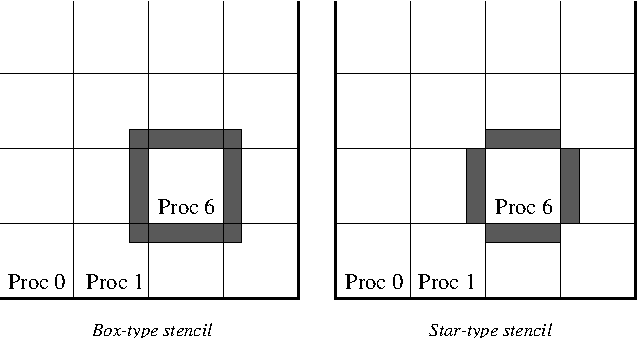
\includegraphics{ghost}}
%\centerline{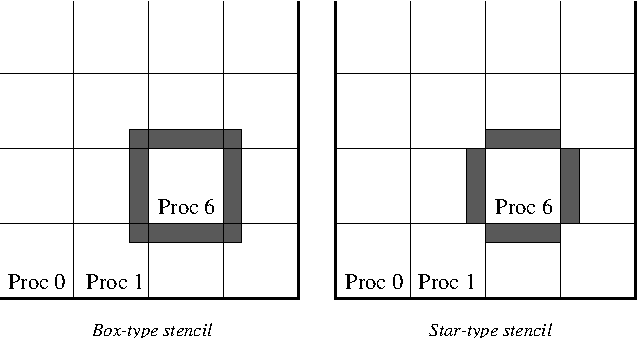
\psfig{file=ghost.eps,angle=0}}
\caption{Ghost Points for Two Stencil Types on the Seventh Process}
\label{fig_ghosts}
\end{figure}

\subsection{Creating Distributed Arrays}

The PETSc DA object manages the parallel communication required
while working with data stored in regular arrays. The actual data
is stored in approriately sized vector objects; the DA object 
only contains the parallel data layout information and communication
information, however it may be used to create vectors and matrices with the
proper layout.

One creates a distributed array communication data structure 
in two dimensions with the command 
\begin{tabbing}
  DACreate2d(MPI\_Comm comm,DAPeriodicType wrap,DAStencilType st,int M,\\
             int N,int m,int n,int dof,int s,int *lx,int *ly,DA *da);
\end{tabbing}
The \findex{DACreate2d()} \sindex{array, distributed} arguments
\sindex{distributed array} \trl{M} and \trl{N} indicate the global
numbers of grid points in each direction, while \trl{m} and \trl{n}
denote the process partition in each direction; \trl{m*n} must equal
the number of processes in the MPI communicator, \trl{comm}.  
Instead of specifying the process layout, one may use
PETSC\_DECIDE for \trl{m} and \trl{n} 
so that PETSc will determine the partition using MPI. The type of
periodicity of the array is specified by \trl{wrap}, which can be 
\trl{DA_NONPERIODIC} \findex{DA_NONPERIODIC} (no periodicity), 
\trl{DA_XYPERIODIC} \findex{DA_XYPERIODIC} (periodic in
both x- and y-directions), \trl{DA_XPERIODIC} \findex{DA_XPERIODIC}, 
or \trl{DA_YPERIODIC}.\findex{DA_YPERIODIC}  The argument \trl{dof} 
indicates the number of degrees of freedom at each array point,
and \trl{s} is the stencil width (i.e., the width of the ghost point region).
The optional arrays \trl{lx} and \trl{ly} may contain the number of nodes
along the x and y axis for each cell, i.e. the dimension of \trl{lx} is
\trl{m} and the dimension of \trl{ly} is \trl{n}; or \trl{PETSC_NULL} 
may be passed in.

Two types of distributed array communication data structures 
can be created, as specified by \trl{st}.
Star-type stencils that radiate outward only in the coordinate
directions are indicated by \trl{DA_STENCIL_STAR},
\findex{DA_STENCIL_STAR} while box-type stencils are specified by
\trl{DA_STENCIL_BOX}. \findex{DA_STENCIL_BOX} For example, for the
two-dimensional case,
\trl{DA_STENCIL_STAR} with width 1 corresponds to the standard 5-point
stencil, while \trl{DA_STENCIL_BOX} with width 1 denotes the
standard 9-point stencil.  In both instances the ghost points are
identical, the only difference being that with star-type stencils
certain ghost points are ignored, decreasing substantially
the number of messages sent.  Note that the \trl{DA_STENCIL_STAR}
stencils can save interprocess communication in two and three
dimensions.

These DA stencils have nothing directly to do with any finite
difference stencils one might chose to use for a discretization; they
only ensure that the correct values are in place for application of a
user-defined finite difference stencil (or any other
discretization technique).

The commands for creating distributed array communication data structures
in one and three dimensions are analogous:
\findex{DACreate3d()} \findex{DACreate1d()} \findex{DACreate3d()}
\begin{tabbing}
  DACreate1d(MPI\_Comm comm,DAPeriodicType wrap,int M,int w,int s,int *lc,DA *inra);\\
  DACreate3d\=(MPI\_Comm comm,DAPeriodicType wrap,DAStencilType stencil\_type,\\
             \>int M,int N,int P,int m,int n,int p,int w,int s,int *lx,int *ly,int *lz,DA *inra);
\end{tabbing}
\trl{DA_ZPERIODIC}, \findex{DA_ZPERIODIC}
\trl{DA_XZPERIODIC}, \findex{DA_XZPERIODIC}
\trl{DA_YZPERIODIC}, and \findex{DA_YZPERIODIC}
\trl{DA_XYZPERIODIC} \findex{DA_XYZPERIODIC}
are additional options in three dimensions for DAPeriodicType.
The routines to create distributed arrays are collective, so that all
processes in the communicator \trl{comm} must call \trl{DACreateXXX()}.

%----------------------------------------------------------------------------------
\subsection{Local/Global Vectors and Scatters}

Each DA object defines the layout of two vectors: a distributed
global vector and a local vector that includes room for the
appropriate ghost points.  The DA object provides information
about the size and layout of these vectors, but does not internally
allocate any associated storage space for field values.  Instead, the
user can create vector objects that use the DA layout
information with the routines
\begin{tabbing}
  DACreateGlobalVector(DA da,Vec *g);\\
  DACreateLocalVector(DA da,Vec *l);
\end{tabbing}
\findex{DACreateGlobalVector()}
\findex{DACreateLocalVector()}
These vectors will generally serve as the building blocks for local
and global PDE solutions, etc.  If additional vectors with such
layout information are needed in a code, they can be obtained by
duplicating \trl{l} or \trl{g} via
VecDuplicate() or VecDuplicateVecs().

We emphasize that a distributed array provides the information needed
to communicate the ghost value information between processes.  In most
cases, several different vectors can share the same communication
information (or, in other words, can share a given DA).  The
design of the DA object makes this easy, as each DA
operation may operate on vectors of the appropriate size, as obtained
via DACreateLocalVector() and DACreateGlobalVector() or as
produced by VecDuplicate().  As such, the DA
scatter/gather operations (e.g., DAGlobalToLocalBegin()) require
vector input/output arguments, as discussed below.

PETSc currently provides no container for multiple arrays sharing the
same distributed array communication; note, however, that the \trl{dof}
parameter handles many cases of interest.

At certain stages of many applications, there is a need to work 
on a local portion of the vector, including the ghost points. 
This may be done by scattering a global vector into its 
local parts by using the two-stage commands
\begin{tabbing}
  DAGlobalToLocalBegin(DA da,Vec g,InsertMode iora,Vec l);\\
  DAGlobalToLocalEnd(DA da,Vec g,InsertMode iora,Vec l);
\end{tabbing}
which allow the overlap of communication and computation.
\findex{DAGlobalToLocalEnd()}  \findex{DAGlobalToLocalBegin()}
Since the global and local vectors, given by \trl{g} and \trl{l}, respectively,
must be compatible with the distributed array, \trl{da}, they should be
generated by DACreateGlobalVector() 
\findex{DACreateGlobalVector()} and DACreateLocalVector()
\findex{DACreateLocalVector()}
(or be duplicates of such a vector obtained via VecDuplicate()).
The InsertMode can be either \trl{ADD_VALUES} or \trl{INSERT_VALUES}.

One can scatter the local patches into the distributed vector
with the command \findex{DALocalToGlobal()}
\begin{tabbing}
  DALocalToGlobal(DA da,Vec l,InsertMode mode,Vec g);
\end{tabbing}
Note that this function is not
subdivided into beginning and ending phases, since it is purely local.

A third type of distributed array scatter is from a local
vector (including ghost points that contain irrelevant values) to 
a local vector with correct ghost point values. 
This scatter may be done by \findex{DALocalToLocalBegin()}
commands \findex{DALocalToLocalEnd()}
\begin{tabbing}
  DALocalToLocalBegin(DA da,Vec l1,InsertMode iora,Vec l2);\\
  DALocalToLocalEnd(DA da,Vec l1,InsertMode iora,Vec l2);
\end{tabbing}
Since both local vectors, \trl{l1} and \trl{l2},
must be compatible with the distributed array, \trl{da}, they should be
generated by DACreateLocalVector() \findex{DACreateLocalVector()}
(or be duplicates of such vectors obtained via VecDuplicate()).
The InsertMode can be either \trl{ADD_VALUES} or \trl{INSERT_VALUES}.

It is possible to directly access the vector scatter contexts (see below)
used in the local-to-global (\trl{ltog}), global-to-local 
(\trl{gtol}), and local-to-local (\trl{ltol})
scatters with the command \findex{DAGetScatter()}
\begin{tabbing}
  DAGetScatter(DA da,VecScatter *ltog,VecScatter *gtol,VecScatter *ltol);
\end{tabbing}
Most users should not need to use these contexts.

\subsection{Local (Ghosted) Work Vectors}
In most applications the local ghosted vectors are only needed during user
``function evaluations''. PETSc provides an easy light-weight (requiring 
essentially no CPU time) way to obtain these work vectors and return them when
they are no longer needed. This is done with the routines
\begin{tabbing}
  DAGetLocalVector(DA da,Vec *l);\\
   .... use the local vector l\\
  DARestoreLocalVector(DA da,Vec *l);
\end{tabbing}

\subsection{Accessing the Vector Entries for DA Vectors}
PETSc provides an easy way to set values into the DA Vectors and access them using
the natural grid indexing. This is done with the routines 
\begin{tabbing}
  DAVecGetArray(DA da,Vec l,void *array);\\
   ... use the array indexing it with 1 or 2 or 3 dimensions \\
   ... depending on the dimension of the DA\\
  DAVecRestoreArray(DA da,Vec l,void *array);
\end{tabbing}
where {\tt array} is a multidimensional C array with the same dimension as
{\tt da}. The vector l can be either a global vector or a local vector.
The {\tt array} is accessed using the usual {\bf global} indexing
on the entire grid, but the user may {\bf only} refer to the local and ghost
entries of this array as all other entries are undefined. For example for a
scalar problem in two dimensions one could do
\begin{tabbing}
   PetscScalar **f,**u;\\
   ...\\
  DAVecGetArray(DA da,Vec local,(void*)\&u);\\
  DAVecGetArray(DA da,Vec global,(void*)\&f);\\
   ...\\
      f[i][j] = u[i][j] - ...\\
   ...\\
  DAVecRestoreArray(DA da,Vec local,(void*)\&u);\\
  DAVecRestoreArray(DA da,Vec global,(void*)\&f);
\end{tabbing}
See \trl{${PETSC_DIR}/src/snes/examples/tutorials/ex5.c} for a 
complete example and see \trl{${PETSC_DIR}/src/snes/examples/tutorials/ex19.c} for an
example for a multi-component PDE.

%---------------------------------------------------------------------------
\subsection{Grid Information}

The global indices of the lower left corner of the local portion of the array 
as well as the local array size can be obtained with the commands
\findex{DAGetCorners()} \findex{DAGetGhostCorners()}
\begin{tabbing}
  DAGetCorners(DA da,int *x,int *y,int *z,int *m,int *n,int *p);\\
  DAGetGhostCorners(DA da,int *x,int *y,int *z,int *m,int *n,int *p);
\end{tabbing}
The first version excludes any ghost points, while the second version
includes them. 
The routine \findex{DAGetGhostCorners()} DAGetGhostCorners()
deals with the fact that subarrays along boundaries of the problem
domain have ghost points only on their interior edges, but not on
their boundary edges.

When either type of stencil is used, \trl{DA_STENCIL_STAR} or 
\trl{DA_STENCIL_BOX}, the local vectors (with the ghost points) 
represent rectangular arrays, including the extra corner elements in 
the \trl{DA_STENCIL_STAR} case. This configuration provides simple 
access to the elements by employing two- (or three-) dimensional indexing. 
The only difference between the 
two cases is that when \trl{DA_STENCIL_STAR} is used, the extra 
corner components are {\em not} scattered between the processes and thus
contain undefined values that should {\em not} be used.

To assemble global stiffness matrices, one needs either 
\begin{itemize}
\item
the global node number of each local node 
including the ghost nodes. This number may be determined by using the 
command \findex{DAGetGlobalIndices()}
\begin{tabbing}
  DAGetGlobalIndices(DA da,int *n,int *idx[]);
\end{tabbing}
The output argument \trl{n} contains the number of 
local nodes, including ghost nodes, while \trl{idx} contains a list of length
\trl{n} containing the global indices that correspond to the local nodes. Either
parameter may be omitted by passing \trl{PETSC_NULL}. Note that the Fortran
interface differs slightly; see Section~\ref{sec_fortranarrays} for details.
\item
or to set up the vectors and matrices so that their entries may be
added using the local numbering. This is done by first calling 
\begin{tabbing}
  DAGetISLocalToGlobalMapping(DA da,ISLocalToGlobalMapping *map);
\end{tabbing}
followed by 
\begin{tabbing}
  VecSetLocalToGlobalMapping(Mat A,ISLocalToGlobalMapping map);\\
  MatSetLocalToGlobalMapping(Mat A,ISLocalToGlobalMapping map);
\end{tabbing}
Now entries may be added to the vector and matrix using the local numbering
and VecSetValuesLocal() and MatSetValuesLocal().
\end{itemize}

Since the global ordering that PETSc uses to manage its parallel vectors 
(and matrices) does not usually correspond to the ``natural'' ordering 
of a two- or three-dimensional array, the DA structure provides 
an application ordering AO (see Section \ref{sec_ao}) that maps 
between the natural ordering on a rectangular grid and the ordering PETSc
uses to parallize. This ordering context can be obtained with the command
\begin{tabbing}
  DAGetAO(DA da,AO *ao);
\end{tabbing}
\findex{DAGetAO()}
In Figure \ref{fig_daao} we indicate the orderings for a two-dimensional distributed 
array, divided among four processes.

\begin{figure}[tb]
\centerline{ 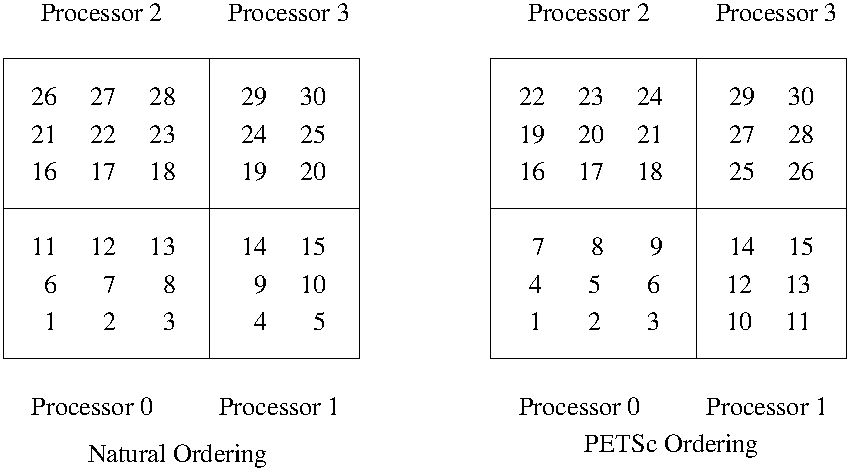
\includegraphics{danumbering}}
%\centerline{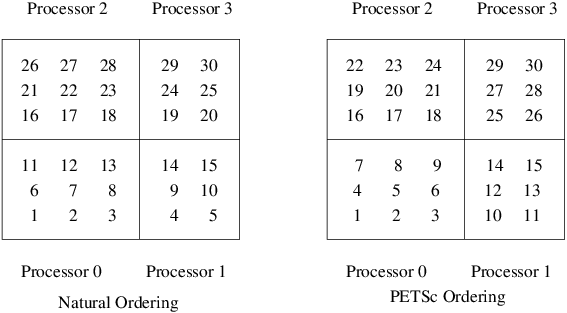
\psfig{file=danumbering.eps,angle=270,width=4.7in}}
\caption{Natural Ordering and PETSc Ordering for a 2D Distributed Array (Four Processes)}
\label{fig_daao}
\end{figure}

The example
\trl{${PETSC_DIR}/src/snes/examples/tutorials/ex5.c},
illustrates the use of a distributed array in the solution of
a nonlinear problem.  The analogous Fortran program is
\break \trl{${PETSC_DIR}/src/snes/examples/tutorials/ex5f.F};
see Chapter \ref{chapter_snes} for a discussion of the nonlinear
solvers.

%\begin{figure}[H]
%{\small
%\fileinclude{../../../../src/snes/examples/tutorials/ex5.c}
%}
%\caption{Use of Distributed Arrays}
%\label{fig_daexample}
%\end{figure}

% -------------------------------------------------------------------------------------- 
\section{Software for Managing Vectors Related to Unstructured Grids}
\label{sec_unstruct}

% -------------------------------------------------------------------------------------- 
\subsection{Index Sets} \sindex{index sets}
\label{sec_indexset}

To facilitate general vector scatters and gathers used, for example, in updating 
ghost points for problems defined on unstructured grids, PETSc employs the 
concept of an index set.  An index set, which is a generalization of a 
set of integer indices, is used to define scatters, gathers, and similar 
operations on vectors and matrices. 

The following command creates a index set based on a list 
of integers: \findex{ISCreateGeneral()}
\begin{tabbing}
  ISCreateGeneral(MPI\_Comm comm,int n,int *indices, IS *is);
\end{tabbing}
This routine essentially copies the \trl{n} indices passed 
to it by the integer array \trl{indices}.  
Thus, the user should be sure to free the integer array \trl{indices} 
when it is no longer needed, perhaps directly after the call to 
ISCreateGeneral(). The communicator, \trl{comm}, should consist of all 
processes that will be using the IS.

Another standard index set is defined by a starting point (\trl{first}) and a
stride (\trl{step}), \sindex{stride} and can be created with the command
\begin{tabbing}
  ISCreateStride(MPI\_Comm comm,int n,int first,int step,IS *is);
\end{tabbing}

Index sets can be destroyed with the command \findex{ISDestroy()}
\begin{tabbing}
  ISDestroy(IS is); 
\end{tabbing}

On rare occasions the user may need to access information directly 
from an index set. \findex{ISGetSize()} 
Several commands \findex{ISStrideGetInfo()} \findex{ISGetIndices()}
assist in this process:
\begin{tabbing}
  ISGetSize(IS is,int *size);\\
  ISStrideGetInfo(IS is,int *first,int *stride);\\
  ISGetIndices(IS is,int **indices);
\end{tabbing}
The function ISGetIndices() returns a pointer to a list of the 
indices in the index set. 
For certain index sets, this may be a 
temporary array of indices created specifically for a given routine. 
Thus, once the user finishes using the array of indices, 
the routine \findex{ISRestoreIndices()}
\begin{tabbing}
  ISRestoreIndices(IS is, int **indices); 
\end{tabbing}
should be called to ensure that the system can free the space it 
may have used to generate the list of indices.

A blocked version of the index sets can be created with the command
\findex{ISCreateBlock}
\begin{tabbing}
  ISCreateBlock(MPI\_Comm comm,int bs,int n,int *indices, IS *is);
\end{tabbing}
This version is used for defining operations in which each element of the index
set refers to a block of \trl{bs} vector entries.  Related routines analogous
to those described above exist as well, including
ISBlockGetIndices(), ISBlockGetSize(), ISBlockGetLocalSize(), ISBlockGetBlockSize(),
and ISBlock(). See the man pages for details.
\findex{ISBlockGetIndices()} \findex{ISBlockGetSize()} \findex{ISBlockGetLocalSize()} \findex{ISBlockGetBlockSize()}
\findex{ISBlock()}

% -------------------------------------------------------------------------------------- 
\subsection{Scatters and Gathers} \sindex{scatter} \sindex{gather}
\label{sec_scatter}

PETSc vectors have full support for general scatters and 
gathers. One can select any subset of the components of a vector to
insert or add to any subset of the components of another vector.
We refer to these operations as generalized scatters, though they are 
actually a combination of scatters and gathers. 

\findex{VecScatterCreate()} \findex{VecScatterBegin()}
\findex{VecScatterEnd()} \findex{VecScatterDestroy()}
\findex{INSERT_VALUES} \findex{SCATTER_FORWARD}
To copy selected components from one vector 
to another, one uses the following set of commands:
\begin{tabbing}
  VecScatterCreate(Vec x,IS ix,Vec y,IS iy,VecScatter *ctx);\\
  VecScatterBegin(VecScatter ctx,Vec x,Vec y,INSERT\_VALUES,SCATTER\_FORWARD);\\
  VecScatterEnd(VecScatter ctx,Vec x,Vec y,INSERT\_VALUES,SCATTER\_FORWARD);\\
  VecScatterDestroy(VecScatter ctx);
\end{tabbing} 
Here \trl{ix} denotes the index set of the first vector, while \trl{
iy} indicates the index set of the destination vector.  The vectors
can be parallel or sequential. The only requirements are that the
number of entries in the index set of the first vector, \trl{ix},
equal the number in the destination index set, \trl{iy}, and that the
vectors be long enough to contain all the indices referred to in the
index sets.  The argument \trl{INSERT_VALUES} specifies that the
vector elements will be inserted into the specified locations of the
destination vector, overwriting any existing values.  To add the
components, rather than insert them, the user should select the option
\trl{ADD_VALUES} \findex{ADD_VALUES} instead of \trl{INSERT_VALUES}.

To perform a conventional gather operation, the user simply makes
 the destination index set, 
\trl{iy}, be a stride index set with a stride of one.  Similarly, a 
conventional scatter can be done with an initial (sending) index set 
consisting of a stride.  The scatter rotines are collective operations
(i.e. all processes that own 
a parallel vector {\em must} call the scatter routines). When scattering from a 
parallel vector to sequential vectors, each process has its own sequential 
vector that receives values from locations as indicated in its own 
index set. Similarly, in scattering
from sequential vectors to a parallel vector, each process has its
own sequential vector that makes contributions to the parallel vector.

{\em Caution}: When \trl{INSERT_VALUES} is used, if two different
processes contribute different values to the same component in a
parallel vector, either value may end up being inserted. When \trl{
ADD_VALUES} is used, the correct sum is added to the correct
location.

In some cases one may wish to ``undo'' a scatter, that is perform the 
scatter backwards switching the roles of the sender and receiver. This is 
done by using 
\begin{tabbing}
  VecScatterBegin(VecScatter ctx,Vec y,Vec x,INSERT\_VALUES,SCATTER\_REVERSE);\\
  VecScatterEnd(VecScatter ctx,Vec y,Vec x,INSERT\_VALUES,SCATTER\_REVERSE);
\end{tabbing} 
\findex{SCATTER_REVERSE} Note that the roles of the first 
two arguments to these routines must be swapped whenever the \trl{SCATTER_REVERSE}
option is used.

Once a VecScatter object has been created it may be used with any vectors
that have the appropriate parallel data layout. That is, one can call 
VecScatterBegin() and VecScatterEnd() with different vectors than 
used in the call to VecScatterCreate() so long as they have the same 
parallel layout (number of elements on each process are the same). Usually,
these ``different'' vectors would have been obtained via calls to 
VecDuplicate() from the original vectors used in the call to 
VecScatterCreate().

\sindex{vector values, getting} \findex{VecGetValues()}
There is a PETSc routine that is nearly the opposite of VecSetValues()
\findex{VecSetValues()}, that is, VecGetValues(), but it can only get
local values from the vector. \findex{VecGetValues()}
To get off process values, the user should create a new vector where
the components are to be stored and perform the appropriate vector 
scatter. For example, if one desires to obtain the values of the 
100th and 200th entries of a parallel vector, \trl{p}, one could use 
a code such as that within Figure~\ref{fig_vecscatter}.
In this example, the values of the 100th and 200th components are
placed in the array 
values. In this example each process now has the 100th and 
200th component, but obviously each process could gather any 
elements it needed, or none by creating an index set with no entries.

\begin{figure}[tb]
\begin{tabbing}
   Vec         p, x;         /* initial vector, destination vector */\\
   VecScatter  scatter;      /* scatter context */\\
   IS          from, to;     /* index sets that define the scatter */\\
   PetscScalar *values;\\
   int         \trl{idx_from[] = {100,200}, idx_to[] = {0,1};}\\

   VecCreateSeq(PETSC\_COMM\_SELF,2,\&x);\\
   ISCreateGeneral(PETSC\_COMM\_SELF,2,idx\_from,\&from);\\
   ISCreateGeneral(PETSC\_COMM\_SELF,2,idx\_to,\&to);\\
   VecScatterCreate(p,from,x,to,\&scatter);\\
   VecScatterBegin(scatter,p,x,INSERT\_VALUES,SCATTER\_FORWARD);\\
   VecScatterEnd(scatter,p,x,INSERT\_VALUES,SCATTER\_FORWARD);\\
   VecGetArray(x,\&values);\\
   ISDestroy(from);\\
   ISDestroy(to); \\
   VecScatterDestroy(scatter);
\end{tabbing}
\caption{Example Code for Vector Scatters}
\label{fig_vecscatter}
\end{figure}

The scatter comprises two stages, in order to allow overlap of 
communication and computation. The introduction of the 
VecScatter context allows the communication patterns for the scatter
to be computed once and then reused repeatedly. Generally, even 
setting up the communication for a scatter requires communication; 
hence, it is best to reuse such information when possible.

% -------------------------------------------------------------------------------
\subsection{Scattering Ghost Values}

The scatters provide a very general method for managing the communication of 
required ghost values for unstructured grid computations. One scatters
the global vector into a local ``ghosted'' work vector, performs the computation
on the local work vectors, and then scatters back into the global solution 
vector. In the simplest case this may be written as
\begin{tabbing}
   Function: (Input Vec globalin, Output Vec globalout)\\
\\
  VecScatterBegin(\=VecScatter scatter,Vec globalin,Vec localin,InsertMode INSERT\_VALUES,\\
                 \>         ScatterMode SCATTER\_FORWARD);\\
  VecScatterEnd(VecScatter scatter,Vec globalin,Vec localin,InsertMode INSERT\_VALUES,\\
                 \>       ScatterMode SCATTER\_FORWARD);\\
  \trl{/*} For example, do local calculations from localin to localout \trl{*/} \\
  VecScatterBegin(VecScatter scatter,Vec localout,Vec globalout,InsertMode ADD\_VALUES,\\
                 \>         ScatterMode SCATTER\_REVERSE);\\
  VecScatterEnd(VecScatter scatter,Vec localout,Vec globalout,InsertMode ADD\_VALUES,\\
                 \>       ScatterMode SCATTER\_REVERSE);
\end{tabbing}

% -------------------------------------------------------------------------------
\subsection{Vectors with Locations for Ghost Values}


There are two minor drawbacks to the basic approach described above:
\begin{itemize}
\item the extra memory requirement for the local work vector, \trl{localin}, which
      duplicates the memory in \trl{globalin}, and
\item the extra time required to copy the local values from \trl{localin} to 
      \trl{globalin}.
\end{itemize}

An alternative approach is to allocate global vectors with space preallocated for 
the ghost values; this may be done with either 
\begin{tabbing}
  VecCreateGhost(MPI\_Comm comm,int n,int N,int nghost,int *ghosts,Vec *vv)
\end{tabbing}
or
\begin{tabbing}
  VecCreateGhostWithArray(MPI\_Comm comm,int n,int N,int nghost,int *ghosts,\\
                                  PetscScalar *array,Vec *vv)
\end{tabbing}
Here \findex{VecCreateGhost()} \findex{VecCreateGhostWithArray()} \trl{n} is the 
number of local vector entries, \trl{N} is the number of \sindex{vectors, with ghost values}
global entries (or \trl{PETSC_NULL}) and \trl{nghost} is the number of 
ghost entries. The array \trl{ghosts} is of size \trl{nghost} and contains the 
global vector location for each local ghost location. Using VecDuplicate()
or VecDuplicateVecs() on a ghosted vector will generate additional ghosted vectors.

In many ways a ghosted vector behaves just like any other \trl{MPI} vector created 
by VecCreateMPI(), the difference is that the ghosted vector has an additional 
``local'' representation that allows one to access the ghost locations. This is done
through the call to \findex{VecGhostGetLocalForm()} 
\begin{tabbing}
 VecGhostGetLocalForm(Vec g,Vec *l);
\end{tabbing}
The vector \trl{l} is a \findex{VecGhostRestoreLocalForm()}
sequential representation of the parallel vector \trl{g} 
that shares the same array space (and hence numerical values); but allows one to 
access the ``ghost'' values past ``the end of the'' array. Note that one access the 
entries in \trl{l} using the local numbering of elements and ghosts, while they 
are accessed in \trl{g} using the global numbering.

A common usage of a ghosted vector is given by
\findex{VecGhostUpdateBegin()} \findex{VecGhostUpdateEnd()}
\begin{tabbing}
  VecGhostUpdateBegin\=(Vec globalin,InsertMode INSERT\_VALUES,\\
                      \>             ScatterMode SCATTER\_FORWARD);\\
  VecGhostUpdateEnd(Vec globalin,InsertMode INSERT\_VALUES,\\
                      \>           ScatterMode SCATTER\_FORWARD);\\
  VecGhostGetLocalForm(Vec globalin,Vec *localin);\\
  VecGhostGetLocalForm(Vec globalout,Vec *localout);\\
   \trl{/*}\\
      Do local calculations from localin to localout \\
   \trl{*/}\\
  VecGhostRestoreLocalForm(Vec globalin,Vec *localin);\\
  VecGhostRestoreLocalForm(Vec globalout,Vec *localout);\\
  VecGhostUpdateBegin(Vec globalout,InsertMode ADD\_VALUES,\\
                        \>            ScatterMode SCATTER\_REVERSE);\\
  VecGhostUpdateEnd(Vec globalout,InsertMode ADD\_VALUES,\\
                        \>          ScatterMode SCATTER\_REVERSE);
\end{tabbing}
      
The routines VecGhostUpdateBegin() and VecGhostUpdateEnd() are equivalent to the routines VecScatterBegin() and VecScatterEnd()
above except that since they are scattering into the ghost locations, they do not need
to copy the local vector values, which are already in place. In addition, the user does not
have to allocate the local work vector, since the ghosted vector already has allocated 
slots to contain the ghost values.

The input arguments \trl{INSERT_VALUES} and \trl{SCATTER_FORWARD}
cause the ghost values to be correctly updated from the appropriate
process. The arguments \trl{ADD_VALUES} and \trl{SCATTER_REVERSE}
update the ``local'' portions of the vector from all the other
processes' ghost values.  This would be appropriate, for example,
when performing a finite element assembly of a load vector.

Section \ref{sec_partitioning} discusses the important topic of partitioning 
an unstructured grid.


%-------------------------------------------------------------
%-------------------------------------------------------------
\cleardoublepage
\chapter{Matrices}
\label{chapter_matrices}
\sindex{matrices}

PETSc provides a variety of matrix implementations because no
single matrix format is appropriate for all problems.  Currently we
support dense storage and compressed sparse row storage (both
sequential and parallel versions), as well as several specialized
formats.  Additional formats can be added.

This chapter describes the basics of using PETSc matrices in general
(regardless of the particular format chosen) and discusses tips for
efficient use of the several simple uniprocess and parallel matrix
types.  The use of PETSc matrices involves the following actions:
create a particular type of matrix, insert values into it, process the
matrix, use the matrix for various computations, and finally destroy
the matrix.  The application code does not need to know or care about
the particular storage formats of the matrices.

\section{Creating and Assembling Matrices}
\label{sec_matcreate}

The simplest routine for forming a PETSc matrix, \trl{A}, is \findex{MatCreate()}
followed by \findex{MatSetSizes()}
\begin{tabbing}
  MatCreate(MPI\_Comm comm,Mat *A)
  MatSetSizes(Mat A,int m,int n,int M,int N)
\end{tabbing}
This routine generates a sequential matrix when running one
process and a parallel matrix for two or more processes; the
particular matrix format is set by the user via options database
commands.  The user specifies either the global matrix dimensions, given
by \trl{M} and \trl{N} or the local dimensions, given by \trl{m} and 
\trl{n} while PETSc completely controls memory allocation.  This routine
facilitates switching among various matrix types, for example, to
determine the format that is most efficient for a certain
application.  By default, MatCreate() employs the sparse AIJ
format, which is discussed in detail Section~\ref{sec_matsparse}.  See
the manual pages for further information about available matrix formats.

To insert or add entries to a matrix, one can call a variant of MatSetValues(), either \findex{MatSetValues()}
\begin{tabbing}
  MatSetValues(\=Mat A,int m,const int idxm[],int n,const int idxn[],const PetscScalar values[],\\
            \>INSERT\_VALUES);
\end{tabbing}
or 
\begin{tabbing}
  MatSetValues(\=Mat A,int m,const int idxm[],int n,const int idxn[],const PetscScalar values[],\\
            \>ADD\_VALUES);
\end{tabbing}
This routine inserts or adds a logically dense subblock of dimension
\trl{m*n} into the 
matrix. The integer indices \trl{idxm} and \trl{idxn}, respectively, indicate the 
global row and column numbers to be inserted.  MatSetValues() uses the 
standard C convention, where the row and column matrix indices begin with 
zero {\em regardless of the storage format employed}.   The array 
\trl{values} is logically two-dimensional, containing the values that are 
to be inserted. By default the values are given in row major order, which is the
opposite of the Fortran convention, meaning that the value to be put in row
\trl{idxm[i]} and column \trl{idxn[j]} is located in \trl{values[i*n+j]}. To
allow the insertion of values in column major order, one can call the command
\findex{MatSetOption()}
\begin{tabbing}
  MatSetOption(Mat A,MAT\_COLUMN\_ORIENTED,PETSC\_TRUE);
\end{tabbing}
{\bf Warning}: Several of the sparse implementations do {\em not} currently
support the column-oriented option.

This notation should not be a mystery to anyone. For example, 
to insert one matrix into another when using Matlab, one uses the command 
\trl{A(im,in) = B;} where \trl{im} and \trl{in} contain the indices for the
rows and columns. This action is identical to the calls above to 
MatSetValues().

When using the block compressed sparse row matrix format (MATSEQBAIJ or
MATMPIBAIJ), one can insert elements more efficiently using the block
variant, MatSetValuesBlocked(). \findex{MatSetValuesBlocked()}

The function MatSetOption() accepts several other inputs; see
the manual page for details.

After the matrix elements have been inserted or added into the matrix, 
they must be processed (also called assembled) before they can be used. The routines for matrix
processing are \findex{MatAssemblyBegin()} \findex{MatAssemblyEnd()}
\begin{tabbing}
  MatAssemblyBegin(Mat A,MAT\_FINAL\_ASSEMBLY);\\
  MatAssemblyEnd(Mat A,MAT\_FINAL\_ASSEMBLY);
\end{tabbing}
By placing other code between these two calls, the user can perform
computations while messages are in transit.
Calls to MatSetValues() with the \trl{INSERT_VALUES} and \trl{
ADD_VALUES} options {\em cannot} be mixed without intervening calls to
the assembly routines.  For such intermediate assembly calls the
second routine argument  typically should be \trl{MAT_FLUSH_ASSEMBLY},
\findex{MAT_FLUSH_ASSEMBLY} which omits some of the work of the full 
assembly process.  \trl{MAT_FINAL_ASSEMBLY} \findex{MAT_FINAL_ASSEMBLY} is
required only in the last matrix assembly before a matrix is used.

Even though one may insert values into PETSc matrices without regard
to which process eventually stores them, for efficiency
reasons we usually recommend generating most entries on the
process where they are destined to be stored.  To help the
application programmer with this task for matrices that are
distributed across the processes by ranges, the routine
\findex{MatGetOwnershipRange()}
\begin{tabbing}
  MatGetOwnershipRange(Mat A,int *first\_row,int *last\_row);
\end{tabbing}
informs the user that all rows from \trl{first_row} to 
\trl{last_row-1} (since the value returned in \trl{last_row} is one more
than the global index of the last local row) will be stored on the local process.

In the sparse matrix implementations, once the assembly routines have been 
called, the matrices are compressed and can be used for matrix-vector
multiplication, etc.
Inserting new values into the matrix at this point will be expensive, 
since it requires copies and possible memory allocation. Thus, whenever 
possible one should completely set the values in the matrices before 
calling the final assembly routines. 

If one wishes to repeatedly assemble matrices that retain the same
nonzero pattern (such as within a nonlinear or time-dependent
problem), the option
\begin{tabbing}
  MatSetOption(Mat A,MAT\_NO\_NEW\_NONZERO\_LOCATIONS,PETSC\_TRUE);
\end{tabbing}
should be specified after the first matrix has been fully assembled.
This option ensures that certain data structures and communication
information will be reused (instead of regenerated) during successive
steps, thereby increasing efficiency.  
See \trl{${PETSC_DIR}/src/ksp/ksp/examples/tutorials/ex5.c} for a simple example of
solving two linear systems that use the same matrix data structure.

\subsection{Sparse Matrices}
\label{sec_matsparse}

\sindex{AIJ matrix format} \sindex{CSR, compressed sparse row format}
The default matrix representation within PETSc is the general sparse
AIJ format (also called the Yale sparse matrix format or compressed
sparse row format, CSR).  This section discusses tips for {\em
efficiently} using this matrix format for large-scale
applications. Additional formats (such as block compressed row and
block diagonal storage, which are generally much more efficient for
problems with multiple degrees of freedom per node) are discussed
below.  Beginning users need not concern themselves initially with
such details and may wish to proceed directly to
Section~\ref{sec_matoptions}.  However, when an application code
progresses to the point of tuning for efficiency and/or generating
timing results, it is {\em crucial} to read this information.

\subsubsection{Sequential AIJ Sparse Matrices}

In the PETSc AIJ matrix formats, we store the nonzero elements
by rows, along with an array of corresponding column numbers and
an array of pointers to the beginning of each row.  Note that the
diagonal matrix entries are stored with the rest of the nonzeros (not
separately). 

To create a sequential AIJ sparse matrix, \trl{A}, 
\findex{MatCreateSeqAIJ()} with \trl{m} rows and \trl{n} columns,
one uses the command
\begin{tabbing}
  MatCreateSeqAIJ(PETSC\_COMM\_SELF,int m,int n,int nz,int *nnz,Mat *A);
\end{tabbing}
where \trl{nz} or \trl{nnz} can be used to preallocate matrix memory,
as discussed below. The user can set \trl{nz=0} and \trl{
nnz=PETSC_NULL} for PETSc to control all matrix memory allocation.

The sequential and parallel AIJ matrix storage formats by default
employ {\em i-nodes} (identical nodes) when possible.  We search for
consecutive rows with the same nonzero structure, thereby reusing
matrix information for increased efficiency.  Related options database
keys are \trl{-mat_no_inode} (do not use inodes) and \trl{
-mat_inode_limit <limit>} (set inode limit (max limit=5)).
Note that problems with a single degree of freedom per grid node
will automatically not use I-nodes.

By default the internal data representation for the AIJ formats employs
zero-based indexing.  For compatibility with standard Fortran storage,
thus enabling use of external Fortran software packages such as
SPARSKIT, \sindex{SPARSKIT} the option \trl{-mat_aij_oneindex}
\findex{-mat_aij_oneindex} enables one-based indexing, where the stored
row and column indices begin at one, not zero.  All user calls to
PETSc routines, regardless of this option, use zero-based indexing.

\subsubsection{Preallocation of Memory for Sequential AIJ Sparse Matrices}

The dynamic process of allocating new memory and copying from the old
storage to the new is {\em intrinsically very expensive}.  Thus, to
obtain good performance when assembling an AIJ matrix, it is crucial
to preallocate the memory needed for the sparse matrix.  The user has
two choices for preallocating matrix memory via MatCreateSeqAIJ(). 

One can use the scalar \trl{nz} to specify the expected
number of nonzeros for each row.  This is generally fine if the number
of nonzeros per row is roughly the same throughout the matrix (or as a
quick and easy first step for preallocation).  If one underestimates
the actual number of nonzeros in a given row, then during the assembly
process PETSc will automatically allocate additional needed space.
However, this extra memory allocation can slow the computation,

If different rows have very different numbers of nonzeros, one
should attempt to indicate (nearly) the exact number of elements
intended for the various rows with the optional array, \trl{nnz} of
length \trl{m}, where \trl{m} is the number of rows, for example
\begin{tabbing}
   int nnz[m];\\
   nnz[0] = \trl{<}nonzeros in row 0\trl{>}\\
   nnz[1] = \trl{<}nonzeros in row 1\trl{>}\\
   ....\\
   nnz[m-1] = \trl{<}nonzeros in row m-1\trl{>}
\end{tabbing}
In this case, the assembly process will require no additional memory
allocations if the \trl{nnz} estimates are correct. If, however,
the \trl{nnz} estimates are incorrect, PETSc will automatically
obtain the additional needed space, at a slight loss of efficiency.

Using the array \trl{nnz} to preallocate memory is especially
important for efficient matrix assembly if the number of nonzeros
varies considerably among the rows.  One can generally set \trl{nnz}
either by knowing in advance the problem structure (e.g., the stencil
for finite difference problems on a structured grid) or by
precomputing the information by using a segment of code similar to
that for the regular matrix assembly.  The overhead of determining the
\trl{nnz} array will be quite small compared with the overhead of the
inherently expensive mallocs and moves of data that are needed for
dynamic allocation during matrix assembly. Always guess high if exact
value is not known (since extra space is cheaper than too little).

Thus, when assembling a sparse matrix with very different
numbers of nonzeros in various rows, one could proceed 
as follows for finite difference methods:
\begin{tabbing}
12\=12\= \kill
    \> - Allocate integer array \trl{nnz}.\\
    \> - Loop over grid, counting the expected number of nonzeros for the row(s)\\
    \>\>  associated with the various grid points.\\
    \> - Create the sparse matrix via MatCreateSeqAIJ() or alternative.\\
    \> - Loop over the grid, generating matrix entries and inserting 
      in matrix via MatSetValues().\\
  \end{tabbing}
\vspace{-0.2in}
For (vertex-based) finite element type calculations, an analogous procedure is as follows:
  \begin{tabbing}
12\=12\= \kill
    \> - Allocate integer array \trl{nnz}.\\
    \>- Loop over vertices, computing the number of neighbor vertices, which determines the\\
    \>\> number of nonzeros for the corresponding matrix row(s).\\
    \> - Create the sparse matrix via MatCreateSeqAIJ() or alternative.\\
    \> - Loop over elements, generating matrix entries and inserting
      in matrix via MatSetValues().\\
  \end{tabbing}

The \trl{-info} \findex{-info} option causes the routines
MatAssemblyBegin() and MatAssemblyEnd() to print
information about the success of the preallocation.  Consider the
following example for the MATSEQAIJ matrix format:
\begin{tabbing}
   MatAssemblyEnd\_SeqAIJ:Matrix size 10 X 10; storage space:20 unneeded, 100 used\\
   MatAssemblyEnd\_SeqAIJ:Number of mallocs during MatSetValues is 0
\end{tabbing}
The first line indicates that the user preallocated 120 spaces but only
100 were used. The second line indicates that the user preallocated
enough space so that PETSc did not have to internally allocate additional
space (an expensive operation).  In the next example the user did not
preallocate sufficient space, as indicated by the fact that the number
of mallocs is very large (bad for efficiency):
\begin{tabbing}
   MatAssemblyEnd\_SeqAIJ:Matrix size 10 X 10; storage space:47 unneeded, 1000 used\\
   MatAssemblyEnd\_SeqAIJ:Number of mallocs during MatSetValues is 40000
\end{tabbing}
 
Although at first glance such procedures for determining the matrix
structure in advance may seem unusual, they are actually very
efficient because they alleviate the need for dynamic
construction of the matrix data structure, which can be very
expensive.


\subsubsection{Parallel AIJ Sparse Matrices}

Parallel sparse matrices with the AIJ 
format can be created with the command \findex{MatCreateMPIAIJ()}
\begin{tabbing}
  MatCreateMPIAIJ\=(MPI\_Comm comm,int m,int n,int M,int N,int d\_nz,\\
                 \>         int *d\_nnz, int o\_nz,int *o\_nnz,Mat *A);
\end{tabbing}
\trl{A} is the newly created matrix, while the arguments \trl{m}, 
\trl{M}, and \trl{N}, indicate the number of local rows and
the number of global rows and columns, respectively. In the PETSc partitioning scheme,
all the matrix columns are local and \trl{n} is the number of columns 
corresponding to local part of a parallel vector.
Either the local or
global parameters can be replaced with PETSC\_DECIDE, so that 
PETSc will determine \findex{PETSC_DECIDE} them.
The matrix is stored with a fixed number of rows on 
each process, given by \trl{m}, or determined by PETSc if \trl{m} is
PETSC\_DECIDE.

If PETSC\_DECIDE is not used for the arguments
\trl{m} and \trl{n}, then the user must ensure that they are chosen to be
compatible with the vectors. To do this, one first considers the matrix-vector product 
$y = A x$. The \trl{m} that is used in the matrix creation routine MatCreateMPIAIJ()
must match the local size used in the vector creation routine VecCreateMPI() for \trl{y}.
Likewise, the \trl{n} used must match that used as the local size in 
VecCreateMPI() for \trl{x}. 

The user must set \trl{d_nz=0}, \trl{o_nz=0}, \trl{d_nnz=PETSC_NULL}, and 
\trl{o_nnz=PETSC_NULL} for PETSc to control dynamic allocation of matrix
memory space.  Analogous to \trl{nz} and \trl{nnz} for the routine 
MatCreateSeqAIJ(), these arguments optionally specify 
nonzero information for the diagonal (\trl{d_nz} and \trl{d_nnz}) and 
off-diagonal (\trl{o_nz} and \trl{o_nnz}) parts of the matrix. 
For a square global matrix, we define each process's diagonal portion 
to be its local rows and the corresponding columns (a square submatrix);  
each process's off-diagonal portion encompasses the remainder of the
local matrix (a rectangular submatrix).  
The rank in the MPI communicator determines the absolute ordering of the
blocks.  That is, the process with rank 0 in the communicator given to  MatCreateMPIAIJ() contains the top rows of the matrix; the i$^{th}$ process
in that communicator contains the i$^{th}$ block of the matrix.

\subsubsection{Preallocation of Memory for Parallel AIJ Sparse Matrices}

As discussed above, preallocation of memory is critical for achieving good
performance during matrix assembly, as this reduces the number of
allocations and copies required.  We present an example for
three processes to indicate how this may be done for the MATMPIAIJ
matrix format.  Consider the 8 by
8 matrix, which is partitioned by default with three rows on the first
process, three on the second and two on the third.  {\small
\[
\left( \begin{array}{cccccccccc} 
1  & 2  & 0  & | & 0  & 3  & 0  & |  & 0  & 4  \\
0  & 5  & 6  & | & 7  & 0  & 0  & |  & 8  & 0 \\
9  & 0  & 10 & | & 11 & 0  & 0  & |  & 12 & 0  \\
\hline \\
13 & 0  & 14 & | & 15 & 16 & 17 & |  & 0  & 0  \\
0  & 18 & 0  & | & 19 & 20 & 21 & |  & 0  & 0 \\
0  & 0  & 0  & | & 22 & 23 & 0  & |  & 24 & 0 \\
\hline \\
25 & 26 & 27 & | & 0  & 0  & 28 & |  & 29 & 0 \\
30 & 0  & 0  & | & 31 & 32 & 33 & |  & 0  &34 
\end{array} \right)
\]
}

The ``diagonal'' submatrix, \trl{d}, on the first process is given by 
{\small
\[
\left( \begin{array}{ccc} 
1  & 2  & 0  \\
0  & 5  & 6  \\
9  & 0  & 10 
\end{array} \right),
\]
}
while the ``off-diagonal'' submatrix, \trl{o}, matrix is given by 
{\small
\[
\left( \begin{array}{ccccc} 
 0  & 3  & 0   & 0  & 4  \\
 7  & 0  & 0   & 8  & 0  \\
 11 & 0  & 0   & 12 & 0  \\
\end{array} \right).
\]
}
For the first process one could set \trl{d_nz} to 2 (since each
row has 2 nonzeros) or, alternatively, set \trl{d_nnz} to \{2,2,2\}.
The \trl{o_nz} could be set to 2 since each row of the \trl{o} matrix
has 2 nonzeros, or \trl{o_nnz} could be set to \{2,2,2\}.

For the second process the \trl{d} submatrix is given by 
{\small
\[
\left( \begin{array}{cccccccccc} 
 15 & 16 & 17 \\
 19 & 20 & 21 \\
 22 & 23 & 0  
\end{array} \right) .
\]
}
Thus, one could set \trl{d_nz} to 3, since the maximum number of
nonzeros in each row is 3, or alternatively one could set \trl{d_nnz} to
\{3,3,2\}, thereby indicating that the first two rows will have 3
nonzeros while the third has 2. The corresponding \trl{o} submatrix for the
second process is
{\small
\[
\left( \begin{array}{cccccccccc} 
13 & 0  & 14 &  0  & 0  \\
0  & 18 & 0  &  0  & 0 \\
0  & 0  & 0  &  24 & 0 \\
\end{array} \right)
\]
}
so that one could set \trl{o_nz} to 2 or \trl{o_nnz} to \{2,1,1\}.

Note that the user never directly works with the \trl{d} and \trl{o}
submatrices, except when preallocating storage space as indicated above.
Also, the user need not preallocate exactly the correct amount of
space; as long as a sufficiently close estimate is given, the high
efficiency for matrix assembly will remain.  

As described above, the option \trl{-info} \findex{-info}
will print information about the success of preallocation during
matrix assembly.  For the MATMPIAIJ and MATMPIBAIJ formats, PETSc will also list
the number of elements owned by on each process that were generated
on a different process.  For example, the statements
\begin{tabbing}
   MatAssemblyBegin\_MPIAIJ:Stash has 10 entries, uses 0 mallocs \\
   MatAssemblyBegin\_MPIAIJ:Stash has 3 entries, uses 0 mallocs \\
   MatAssemblyBegin\_MPIAIJ:Stash has 5 entries, uses 0 mallocs 
\end{tabbing}
indicate that very few values have been generated on different processes.
On the other hand, the statements
\begin{tabbing}
   MatAssemblyBegin\_MPIAIJ:Stash has 100000 entries, uses 100 mallocs \\
   MatAssemblyBegin\_MPIAIJ:Stash has 77777 entries, uses 70 mallocs
\end{tabbing}
indicate that many values have been generated on the ``wrong'' processes.
This situation can be very inefficient, since the transfer of values
to the ``correct'' process is generally expensive.  By using the command
MatGetOwnershipRange() in application codes, the user should be able
to generate most entries on the owning process.

{\em Note}: It is fine to generate some entries on the ``wrong'' process. Often
this can lead to cleaner, simpler, less buggy codes.  One should never
make code overly complicated in order to generate all values locally. Rather,
one should organize the code in such a way that {\em most} values are generated locally.

\subsection{Dense Matrices}
\label{sec_matdense}

PETSc provides both sequential and parallel dense matrix formats,
where each process stores its entries in a column-major array in the
usual Fortran style.  To create a sequential, dense PETSc matrix,
\trl{A} of dimensions \trl{m} by \trl{n}, the user should
call \findex{MatCreateSeqDense()}
\begin{tabbing}
  MatCreateSeqDense(PETSC\_COMM\_SELF,int m,int n,PetscScalar *data,Mat *A);
\end{tabbing}
The variable \trl{data} enables the user to optionally provide the
location of the data for matrix storage (intended for Fortran users who
wish to allocate their own storage space).  Most users should merely
set \trl{data} to \trl{PETSC_NULL} for PETSc to control matrix memory allocation.
To create a parallel, dense matrix, \trl{A}, the user should call
\begin{tabbing}
  MatCreateMPIDense(MPI\_Comm comm,int m,int n,int M,int N,PetscScalar *data,Mat *A)
\end{tabbing}
The arguments \trl{m}, \trl{n}, 
\trl{M}, and \trl{N}, indicate the number of local rows and columns and
the number of global rows and columns, respectively. Either the local or
global parameters can be replaced with PETSC\_DECIDE, so that 
PETSc will determine \findex{PETSC_DECIDE} them.
The matrix is stored with a fixed number of rows on 
each process, given by \trl{m}, or determined by PETSc if \trl{m} is
PETSC\_DECIDE. 

PETSc does not provide parallel dense direct solvers. Our focus is on 
sparse iterative solvers.

\section{Basic Matrix Operations}
\label{sec_matoptions}

Table \ref{fig_matrixops} summarizes basic PETSc matrix operations.
We briefly discuss a few of these routines in more detail below.

The parallel matrix can multiply a vector with \trl{n} 
local entries, returning a vector with \trl{m} local entries. That is, 
to form the product \findex{MatMult()}
\begin{tabbing}
  MatMult(Mat A,Vec x,Vec y);
\end{tabbing}
the vectors \trl{x} and \trl{y} should be generated with 
\begin{tabbing}
  VecCreateMPI(MPI\_Comm comm,n,N,\&x);\\
  VecCreateMPI(MPI\_Comm comm,m,M,\&y);
\end{tabbing}
By default, if the user lets PETSc decide the number of components to
be stored locally (by passing in PETSC\_DECIDE as the second
argument to VecCreateMPI() or using VecCreate()), vectors
and matrices of the same dimension are automatically compatible for
parallel matrix-vector operations.

Along with the matrix-vector multiplication routine, there is 
a version for the transpose of the matrix, \findex{MatMultTranspose()}
\begin{tabbing}
  MatMultTranspose(Mat A,Vec x,Vec y);
\end{tabbing}
There are also versions that add the result
to another vector: \findex{MatMultAdd()} \findex{MatMultTransposeAdd()}
\begin{tabbing}
  MatMultAdd(Mat A,Vec x,Vec y,Vec w);\\
  MatMultTransposeAdd(Mat A,Vec x,Vec y,Vec w);
\end{tabbing}
These routines, respectively, produce $ w = A*x + y $ and $ w = A^{T}*x + y$ . 
In C it is legal for the vectors \trl{y} and \trl{w} to be identical.
In Fortran, this situation is forbidden by the language standard, 
but we allow it anyway.

One can print a matrix (sequential or parallel) to the screen with the 
command \findex{MatView()}
\begin{tabbing}
  MatView(Mat mat,PETSC\_VIEWER\_STDOUT\_WORLD);
\end{tabbing}
Other viewers can be used as well. For instance, one can draw the
nonzero stucture of the matrix into the default X-window with the 
command 
\begin{tabbing}
  MatView(Mat mat,PETSC\_VIEWER\_DRAW\_WORLD);
\end{tabbing}
Also one can use \findex{PETSC_VIEWER_DRAW_WORLD}
\begin{tabbing}
  MatView(Mat mat,PetscViewer viewer);
\end{tabbing}
where \trl{viewer} was obtained with PetscViewerDrawOpen().
\findex{PetscViewerDrawOpen()} 
Additional viewers \findex{MatCopy()} and options are given in the MatView() man
page and Section~\ref{sec_viewers}.

\begin{table}[tb]
\begin{center}
\begin{tabular}{ll}
{\bf Function Name} & {\bf Operation} \\
\hline
MatAXPY(Mat Y, PetscScalar a,Mat X,MatStructure); & $ Y = Y + a*X $ \\
MatMult(Mat A,Vec x, Vec y); & $ y = A*x $ \\
MatMultAdd(Mat A,Vec x, Vec y,Vec z); & $ z = y + A*x $ \\
MatMultTranspose(Mat A,Vec x, Vec y); & $ y = A^{T}*x $ \\
MatMultTransposeAdd(Mat A,Vec x, Vec y,Vec z); & $ z = y + A^{T}*x $ \\
MatNorm(Mat A,NormType type,  double *r); & $ r = ||A||_{type}$ \\
MatDiagonalScale(Mat A,Vec l,Vec r); & $ A = \hbox{diag}(l)*A*\hbox{diag}(r) $ \\
MatScale(Mat A,PetscScalar a); & $ A = a*A $ \\
MatConvert(Mat A,MatType type,Mat *B); & $ B = A $ \\
MatCopy(Mat A,Mat B,MatStructure); &  $ B = A $ \\
MatGetDiagonal(Mat A,Vec x); & $ x = \hbox{diag}(A)$ \\
MatTranspose(Mat A,MatReuse,Mat* B); & $ B = A^{T} $ \\
MatZeroEntries(Mat A); & $ A = 0 $ \\
MatShift(Mat Y,PetscScalar a); & $ Y =  Y + a*I $ \\
\hline 
\end{tabular}
\end{center}
\caption{\hbox{PETSc Matrix Operations}}
\label{fig_matrixops}
\end{table}
The NormType argument to MatNorm() is one of \findex{MatNorm()}
\findex{NormType} \trl{NORM_1}, \trl{NORM_INFINITY}, and \trl{NORM_FROBENIUS}.
\findex{NORM_1}  \findex{NORM_INFINITY} \findex{NORM_FROBENIUS}
\sindex{1-norm} \sindex{infinity norm} \sindex {Frobenius norm}
\section{Matrix-Free Matrices} \sindex{matrix-free methods}
\label{sec_matrixfree}
Some people like to use matrix-free methods, which do not require
explicit storage of the matrix, for the numerical solution of partial
differential equations.  To support matrix-free methods in PETSc, one
can use the following command to create a Mat structure without
ever actually generating the matrix:
\findex{MatCreateShell()}
\begin{tabbing}
  MatCreateShell(MPI\_Comm comm,int m,int n,int M,int N,void *ctx,Mat *mat);
\end{tabbing}
Here \trl{M} and \trl{N} are the global matrix dimensions (rows and
columns), \trl{m} and \trl{n} are the local matrix dimensions, and
\trl{ctx} is a pointer to data needed by any user-defined shell matrix
operations; the manual page has additional details about these
parameters.  Most matrix-free algorithms require only the application
of the linear operator to a vector. To provide this action, the user
must write a routine with the calling sequence
\begin{tabbing}
  UserMult(Mat mat,Vec x,Vec y);
\end{tabbing}
and then associate it with the matrix, \trl{mat}, by using the 
command \findex{MatShellSetOperation()}
\begin{tabbing}
  MatShellSetOperation\=(Mat mat,MatOperation MATOP\_MULT,\\
                      \>         (void(*)(void)) PetscErrorCode (*UserMult)(Mat,Vec,Vec));
\end{tabbing}
Here \trl{MATOP_MULT} is the name of the operation for matrix-vector
multiplication. Within each user-defined routine (such as
\trl{UserMult()}), the user should call \findex{MatShellGetContext()}
MatShellGetContext() to obtain the user-defined context, \trl{ctx},
that was set by MatCreateShell().
This shell matrix can be used with the iterative linear
equation solvers discussed in the following chapters.

The routine MatShellSetOperation() can be used to set any other
matrix operations as well.  The file 
\trl{${PETSC_DIR}/include/petscmat.h} provides a complete list of matrix
operations, which have the form \trl{MATOP_<OPERATION>}, where \trl{
<OPERATION>} is the name (in all capital letters) of the user
interface routine (for example, MatMult() $ \to $ \trl{MATOP_MULT}).  All
user-provided functions have the same calling sequence as the
usual matrix interface routines, since the user-defined functions are
intended to be accessed through the same interface, e.g., 
MatMult(Mat,Vec,Vec) $ \to$ \trl{UserMult(Mat,Vec,Vec)}.
The final argument for MatShellSetOperation() needs to be cast
to a \trl{void *}, since the final argument could (depending on the 
MatOperation) be a variety of different functions.

Note that MatShellSetOperation() can also be used as a
``backdoor'' means of introducing user-defined changes in matrix
operations for other storage formats (for example, to override the
default LU factorization routine supplied within PETSc for the
MATSEQAIJ format).  However, we urge anyone who introduces such
changes to use caution, since it would be very easy to
accidentally create a bug in the new routine that could affect
other routines as well.

See also Section~\ref{sec_nlmatrixfree} for details on one set of
helpful utilities for using the matrix-free approach for nonlinear
solvers.

\section{Other Matrix Operations}
\label{sec_othermat}

In many iterative calculations (for instance, in a nonlinear equations
solver), it is important for efficiency purposes to reuse the nonzero 
structure of a matrix, rather than determining it anew every time 
the matrix is generated.  To retain a given matrix but reinitialize
its contents, one can employ \findex{MatZeroEntries()}
\begin{tabbing}
  MatZeroEntries(Mat A);
\end{tabbing}
This routine will zero the matrix entries in the 
data structure but keep all the data that indicates where the nonzeros
are located.  In this way a new matrix assembly will be much less 
expensive, since no memory allocations or copies will be needed. 
Of course, one can also explicitly set selected matrix elements to zero
by calling MatSetValues().

By default, if new entries are made in locations where no nonzeros 
previously existed, space will be allocated for the new entries. 
To prevent the allocation of additional memory and simply discard those 
new entries, one can use the option \findex{MatSetOption()}
\begin{tabbing}
  MatSetOption(Mat A,MAT\_NO\_NEW\_NONZERO\_LOCATIONS,PETSC\_TRUE);
\end{tabbing}
Once the matrix has been assembled, one can factor it numerically
without repeating the ordering or the symbolic factorization. 
This option can save some computational time, although it
does require that the factorization is not done in-place.

In the numerical solution of elliptic partial differential equations,
it can be cumbersome to deal with Dirichlet boundary 
\sindex{boundary conditions} conditions. In
particular, one would like to assemble the matrix without regard to 
boundary conditions and then at the end apply the Dirichlet boundary 
conditions. 
In numerical analysis classes this process is usually presented as moving the 
known boundary conditions to the right-hand side and then solving a smaller
linear system for the interior unknowns. Unfortunately, implementing this
requires extracting a large submatrix from the original matrix and 
creating its corresponding data structures. This process can be expensive 
in terms of both time and memory. 

One simple way to deal with this difficulty is to replace those rows in the 
matrix associated with known boundary conditions, by rows of the 
identity matrix (or some scaling of it). This action can be done with 
the command \findex{MatZeroRows()}
\begin{tabbing}
  MatZeroRowsIS(Mat A,PetscInt numRows,PetscInt rows[],PetscScalar diag\_value),
\end{tabbing}
or equivalently,
\begin{tabbing}
  MatZeroRowsIS(Mat A,IS rows,PetscScalar diag\_value);
\end{tabbing}
For sparse matrices this removes the data structures for certain rows 
of the matrix. If the pointer \trl{diag_value} is \trl{PETSC_NULL}, it 
even removes the diagonal entry. If the pointer is not null, it uses that 
given value at the pointer location 
in the diagonal entry of the eliminated rows. 

One nice feature of this approach is that when solving a nonlinear problem 
such that at each iteration the Dirichlet boundary conditions are in the 
same positions and the matrix retains the same nonzero structure, the user 
can call MatZeroRows() in the first iteration. Then, before generating 
the matrix in the second iteration the user should call
\begin{tabbing}
  MatSetOption(Mat A,MAT\_NO\_NEW\_NONZERO\_LOCATIONS,PETSC\_TRUE);
\end{tabbing}
From that point, \findex{MatSetOption()}
no new values will be inserted into those (boundary) rows of 
the matrix. \findex{MAT_NEW_NONZERO_LOCATIONS} 

Another matrix routine of interest is \findex{MatConvert()}
\begin{tabbing}
  MatConvert(Mat mat,MatType newtype,Mat *M)
\end{tabbing}
which converts the matrix \trl{mat} to new matrix, \trl{M}, that has
either the same or different format.  Set \trl{newtype} to MATSAME
to copy the matrix, keeping the same matrix format.  See 
\trl{${PETSC_DIR}/include/petscmat.h} for other available matrix types;
standard ones are MATSEQDENSE, MATSEQAIJ, MATMPIAIJ, 
               MATSEQBAIJ and MATMPIBAIJ.

In certain applications it may be necessary for application codes
to directly access elements of a matrix. This may be done by using the 
the command (for local rows only)
\begin{tabbing}
  MatGetRow(Mat A,int row, int *ncols,const PetscInt (*cols)[],const PetscScalar (*vals)[]);
\end{tabbing}
The argument \trl{ncols} returns the number of nonzeros in that row, 
while \trl{cols} and \trl{vals} returns the column indices (with indices
starting at zero) and values in the row. If only the column 
indices are needed (and not the corresponding matrix elements), one
can use \trl{PETSC_NULL} for the \trl{vals} argument. Similarly,
one can use \trl{PETSC_NULL} for the \trl{cols} argument.
The user can only examine the values extracted with MatGetRow();
the values {\em cannot} be altered. 
\findex{MatGetRow()} \findex{MatRestoreRow()}
To change the matrix entries, one must use MatSetValues().

Once the user has finished using a row, he or she {\em must} call 
\begin{tabbing}
  MatRestoreRow(Mat A,int row,int *ncols,int **cols,PetscScalar **vals);
\end{tabbing}
to free any space that was allocated during the call to MatGetRow().

% ------------------------------------------------------------------
\section{Partitioning}
\label{sec_partitioning} \sindex{partitioning} \sindex{grid partitioning}

For almost all unstructured grid computation, the distribution of portions of 
the grid across the process's work load and memory can have a very large
impact on performance. In most PDE calculations the grid partitioning and 
distribution across the processes can (and should) be done in a ``pre-processing'' step
before the numerical computations. However, this does not mean it need be done
in a separate, sequential program, rather it should be done before one sets up the 
parallel grid data structures in the actual program. PETSc provides an interface to
the ParMETIS (developed by George Karypis; see the docs/installation/index.htm file
for directions on installing PETSc to use ParMETIS) to allow the partitioning to be done in
parallel. PETSc does not currently provide directly support for dynamic
repartitioning, load balancing by migrating matrix entries between processes, etc.
For problems that require mesh refinement, PETSc uses the ``rebuild the data structure''
approach, as opposed to the ``maintain dynamic data structures that support the 
insertion/deletion of additional vector and matrix rows and columns entries'' approach.

Partitioning in PETSc is organized around the MatPartitioning object. \findex{MatPartitioning}
One first creates a parallel matrix that contains the connectivity information about the 
grid (or other graph-type object) that is to be partitioned. This is done with the 
command
\begin{tabbing}
 MatCreateMPIAdj(\=MPI\_Comm comm,int mlocal,int n,const int ia[],const int ja[],\\
                 \>        int *weights,Mat *Adj);
\end{tabbing}
The argument \trl{mlocal} indicates the number of rows of the graph being provided
by the given process, \trl{n} is the total number of columns; equal to the 
sum of all the \trl{mlocal}. The arguments \trl{ia} and \trl{ja} are the row pointers
and column pointers for the given rows, these are the usual format for parallel 
compressed sparse row storage, using indices starting at 0, {\bf not} 1.

\begin{figure}[H]
\centerline{ 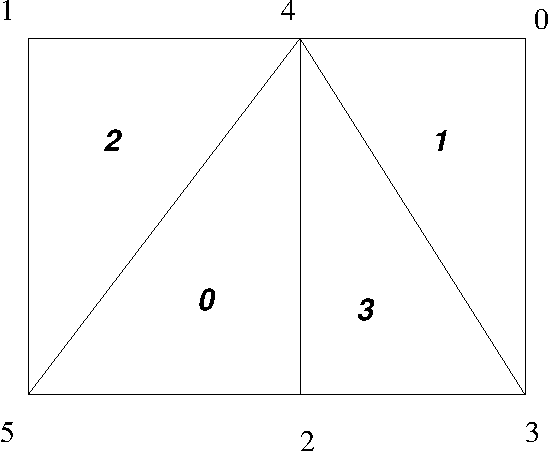
\includegraphics{usg.pdf}}
%\centerline{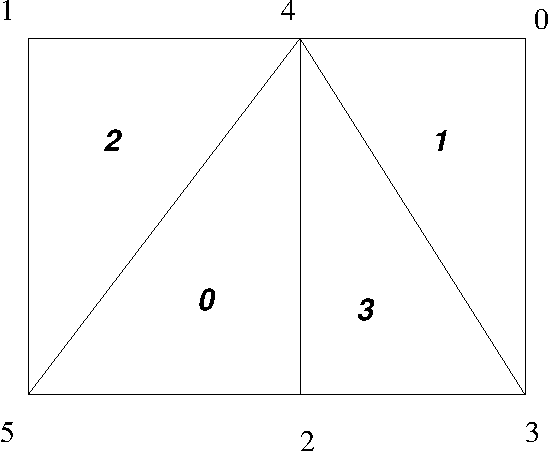
\psfig{file=usg.ps,angle=0}}
\caption{Numbering on Simple Unstructured Grid}
\label{fig_usg}
\end{figure}

This, of course, assumes that one has already distributed the grid (graph) information
among the processes. The details of this initial distribution is not important; it 
could be simply determined by assigning to the first process the first $n_0$ nodes
from a file, the second process the next $ n_1$ nodes, etc.

For example, we demonstrate the form of the \trl{ia} and \trl{ja} for a triangular
grid where we 

(1) partition by element (triangle) 
\begin{itemize}
  \item Process 0, $ mlocal = 2, n = 4, ja = \{2, 3,| 3\}, ia = \{0, 2, 3\} $
  \item Process 1, $ mlocal = 2, n = 4, ja = \{0, | 0, 1\}, ia = \{0, 1, 3\} $
\end{itemize}
Note that elements are not connected to themselves and we only indicate edge connections
(in some contexts single vertex connections between elements may also be included). We use a
$ | $ above to denote the transition between rows in the matrix.

and (2) partition by vertex.
\begin{itemize}
  \item Process 0, $ mlocal = 3, n = 6, ja = \{3, 4, | 4, 5, | 3, 4, 5\}, ia = \{0, 2, 4, 7\} $
  \item Process 1, $ mlocal = 3, n = 6, ja = \{0, 2, 4, |  0, 1, 2, 3, 5,|  1, 2, 4\}, ia = \{0, 3, 8, 11\}. $
\end{itemize}



Once the connectivity matrix has been created the following code will generate the 
renumbering required for the new partition
\begin{tabbing}
 MatPartitioningCreate(MPI\_Comm comm,MatPartitioning *part);\\
 MatPartitioningSetAdjacency(MatPartitioning part,Mat Adj);\\
 MatPartitioningSetFromOptions(MatPartitioning part);\\
 MatPartitioningApply(MatPartitioning part,IS *is);\\
 MatPartitioningDestroy(MatPartitioning part); \\
 MatDestroy(Mat Adj);\\
 ISPartitioningToNumbering(IS is,IS *isg);
\end{tabbing}
The \findex{MatPartitioningCreate()} \findex{MatPartitioningSetAdjacency()} 
\findex{MatPartitioningSetFromOptions()} \findex{MatPartitioningApply()} 
\findex{MatPartitioningDestroy()}  resulting \trl{isg} contains for each local node the new global
number of that node. The resulting \trl{is} contains the new process number
that each local node has been assigned to.

Now that a new numbering of the nodes has been determined one must 
renumber all the nodes and migrate the grid information to the correct process.
The command
\begin{tabbing}
 AOCreateBasicIS(isg,PETSC\_NULL,\&ao);
\end{tabbing}
generates, see Section \ref{sec_ao}, an AO object that can be used in conjunction with the
\trl{is} and \trl{gis} to move the relevant grid information to the correct process
and renumber the nodes etc. 

PETSc does not currently provide tools that completely manage the migration and 
node renumbering, since it will be dependent on the particular data structure you 
use to store the grid information and the type of grid information that you need
for your application. We do plan to include more support for this in the future,
but designing the appropriate general user interface and providing a scalable
implementation that can be used for a wide variety of different grids requires a
great deal of time.

 


% ------------------------------------------------------------------
\cleardoublepage
\chapter{KSP: Linear Equations Solvers} \sindex{linear system solvers}
\label{ch_ksp}

The object KSP is the heart of PETSc, because it provides uniform and efficient access 
to all of the package's linear system solvers, including parallel and sequential,
direct and iterative.
KSP is intended for solving nonsingular systems of the form
\begin{equation}
   A x = b,
\label{eq_Ax=b}
\end{equation}
where $ A$ denotes the matrix representation of a linear operator, $b$
is the right-hand-side vector, and $ x $ is the solution vector.  KSP
uses the same calling sequence for both direct and iterative solution
of a linear system.  In addition, particular solution techniques and
their associated options can be selected at runtime.

The combination of a Krylov subspace method and a preconditioner is at
the center of most modern numerical codes for the iterative solution of
linear systems.  See, for example, \cite{fgn} for an overview of the theory
of such methods.  KSP creates a simplified interface to the
lower-level KSP and PC modules within the PETSc package.  The KSP package,
discussed in
Section~\ref{sec_ksp}, provides many popular Krylov
\sindex{Krylov subspace methods} subspace iterative methods;
the PC module, described in Section~\ref{sec_pc}, includes a
variety of preconditioners.  Although both  KSP and PC can be used
directly, users should employ the interface of KSP.

\section{Using KSP} 
\label{sec_usingsles}

To solve a linear system with KSP, one must first create a solver context 
with the command \findex{KSPCreate()}
\begin{tabbing}
  KSPCreate(MPI\_Comm comm,KSP *ksp); 
\end{tabbing}
Here \trl{comm} is the MPI communicator, and \trl{ksp} is the newly
formed solver context.
Before actually solving a linear system with KSP, the user must call 
the following routine to set the matrices associated with the linear
system: \findex{KSPSetOperators()}
\begin{tabbing}
  KSPSetOperators(KSP ksp,Mat Amat,Mat Pmat,MatStructure flag);
\end{tabbing}
The argument \trl{Amat}, representing the matrix that defines the
linear system, is a symbolic place holder for any kind of matrix.  
In particular, KSP {\em does} support matrix-free methods. 
\sindex{matrix-free methods}
The routine MatCreateShell() \findex{MatCreateShell()}
in Section~\ref{sec_matrixfree} provides further information regarding
matrix-free methods. 
Typically the {\em preconditioning matrix} (i.e., the matrix from which the
preconditioner is to be constructed), \trl{Pmat}, is the same as
the matrix that defines the linear system, \trl{Amat}; however,
occasionally these matrices differ (for instance, \sindex{preconditioning}
when a preconditioning matrix is obtained from a lower order method than 
that employed to form the linear system matrix).
The argument \trl{flag} can be used to eliminate unnecessary work when
repeatedly solving linear systems of the same size with the same 
preconditioning method; when solving just one linear system, this flag is
ignored.  The user can set \trl{flag} as follows:
\begin{itemize}
\item \trl{SAME_NONZERO_PATTERN} - the preconditioning matrix has the
    same \findex{SAME_NONZERO_PATTERN} nonzero structure during successive
    linear solves,
\item \trl{DIFFERENT_NONZERO_PATTERN} - the preconditioning matrix does
     not have the same nonzero structure during successive linear solves,
   \findex{DIFFERENT_NONZERO_PATTERN}
\item \trl{SAME_PRECONDITIONER} - the preconditioner matrix is identical
   to that of the previous linear solve. \findex{SAME_PRECONDITIONER}
\end{itemize}
If the structure of a matrix is not known a priori, one should use
the flag \trl{DIFFERENT_NONZERO_PATTERN}.
 
Much of the power of KSP can be accessed through the single routine
\begin{tabbing}
  KSPSetFromOptions(KSP ksp);
\end{tabbing}
This \findex{KSPSetFromOptions()}
routine accepts the options \trl{-h} and \trl{-help} as well as 
any of the KSP and PC options discussed below. 
To solve a linear system, one sets the rhs and solution vectors using
and executes the
command \findex{KSPSolve()}
\begin{tabbing}
  KSPSolve(KSP ksp,Vec b,Vec x);
\end{tabbing}
where \trl{b} and \trl{x} respectively denote the right-hand-side and
solution vectors.  On return, the iteration number at which convergence
was successfully reached can be obtained using \findex{KSPGetIterationNumber()}.
\begin{tabbing}
  KSPGetIterationNumber(KSP ksp, int *its);
\end{tabbing}
If the iteration diverged, then the {\em negative} of the iteration at
which divergence or breakdown was detected is returned in \trl{its}.
 Section~\ref{section_convergencetests} gives more details regarding
convergence testing. Note that multiple linear solves can be performed by
the same KSP context. Once the KSP context is no longer needed, it should be
destroyed with the command \findex{KSPDestroy()}
\begin{tabbing}
  KSPDestroy(KSP ksp);
\end{tabbing}

The above procedure is sufficient for general use of the KSP package.
One additional step is required for users who wish to customize certain 
preconditioners (e.g., see Section~\ref{sec_bjacobi}) or to log certain 
performance data using the PETSc profiling facilities (as discussed in 
Chapter~\ref{ch_profiling}).
In this case, the user can optionally explicitly call \findex{KSPSetUp()}
\begin{tabbing}
  KSPSetUp(KSP ksp)
\end{tabbing}
before calling KSPSolve() to perform any setup required for 
the linear solvers.  The explicit call of this routine enables the
separate monitoring of any computations performed during the set up
phase, such as incomplete factorization for the ILU preconditioner.

The default solver within KSP is restarted GMRES, preconditioned for
the uniprocess case with ILU(0), and for the multiprocess case
with the block Jacobi method (with one block per process, each of
which is solved with ILU(0)). A variety of other solvers
and options are also available.
To allow application programmers to set any of the preconditioner or 
Krylov subspace options directly within the code, we provide routines
that extract the PC and KSP contexts, \findex{KSPGetPC()}
\begin{tabbing}
  KSPGetPC(KSP ksp,PC *pc);\\
\end{tabbing}
The application programmer can then directly call any of the PC or KSP 
routines to modify the corresponding default options.   

To solve a linear system with a direct solver (currently supported 
by PETSc for sequential matrices, and by several external solvers through
PETSc interfaces (see Section~\ref{sec_externalsol})) one may use the options
\trl{-ksp_type} \trl{preonly} \trl{-pc_type} \trl{lu} 
(see below).

By default, if a direct solver is used, the factorization is {\em not} done 
in-place. This approach prevents the user from the unexpected surprise
of having a corrupted matrix after a linear solve. The routine 
PCFactorSetUseInPlace(), discussed below, causes factorization to 
be done in-place. \findex{PCFactorSetUseInPlace()} 

\section{Solving Successive Linear Systems}

When solving multiple linear systems of the same size with the same
method, several options are available.  To solve successive linear
systems having the {\em same} preconditioner matrix (i.e., the same
data structure with exactly the same matrix elements) but different
right-hand-side vectors, the user should simply call KSPSolve,()
multiple times.  The preconditioner setup operations (e.g.,
factorization for ILU) will be done during the first call to KSPSolve() only; such operations will {\em not} be repeated for
successive solves.

To solve successive linear systems that have {\em different}
preconditioner matrices (i.e., the matrix elements and/or the matrix
data structure change), the user {\em must} call 
KSPSetOperators() and KSPSolve() for each solve.  See
Section~\ref{sec_usingsles} for a description of various flags for
KSPSetOperators() that can save work for such cases.

\section{Krylov Methods}\sindex{Krylov subspace methods}
\label{sec_ksp}

The Krylov subspace methods accept a number of options, many of which 
are discussed below.  First, to set the Krylov subspace method that is to 
be used, one calls the command \findex{KSPSetType()}
\begin{tabbing}
  KSPSetType(KSP ksp,KSPType method);
\end{tabbing}
The type can be one of KSPRICHARDSON, KSPCHEBYCHEV, KSPCG, KSPGMRES, 
KSPTCQMR, KSPBCGS, KSPCGS, KSPTFQMR, KSPCR, KSPLSQR, KSPBICG, or KSPPREONLY.
\findex{KSPRICHARDSON} \findex{KSPCHEBYCHEV} \findex{KSPCG}
\findex{KSPGMRES} \findex{KSPTCQMR} \findex{KSPBCGS} \findex{KSPTFQMR}
\findex{KSPCR} \findex{KSPPREONLY} \findex{KSPBICG}
The KSP method can also be set with the options database command 
\trl{-ksp_type},
followed by one of the options \trl{richardson}, \trl{chebychev}, \trl{cg}, \trl{gmres}, \trl{tcqmr}, 
\trl{bcgs}, \trl{cgs}, \trl{tfqmr}, \trl{cr}, \trl{lsqr}, \trl{bicg}, or \trl{preonly.} \findex{-ksp_type}
There are method-specific options for the Richardson, Chebychev,
and GMRES \findex{KSPChebychevSetEigenvalues()} \findex{KSPGMRESSetRestart()}
methods: \findex{KSPRichardsonSetScale()}  \sindex{GMRES} \sindex{CG}
\begin{tabbing}
  KSPRichardsonSetScale(KSP ksp,double damping\_factor);\\
  KSPChebychevSetEigenvalues(KSP ksp,double emax,double emin);\\
  KSPGMRESSetRestart(KSP ksp,int max\_steps);
\end{tabbing}
The default parameter values are \trl{damping_factor=1.0, 
emax=0.01, emin=100.0}, and \trl{max_steps=30}. The GMRES 
\sindex{restart} restart and Richardson damping factor
can also be set with the options \trl{-ksp_gmres_restart <n>}
and \trl{-ksp_richardson_scale <factor>}. \findex{-ksp_gmres_restart} 
\findex{-ksp_richardson_scale}

The default technique for orthogonalization of the Hessenberg
matrix in GMRES is 
the
unmodified (classical) Gram-Schmidt method, which can be set \sindex{Gram-Schmidt}
with \findex{KSPGMRESSetOrthogonalization()} 
\findex{KSPGMRESClassicalGramSchmidtOrthogonalization}
\begin{tabbing}
  KSPGMRESSetOrthogonalization(KSP ksp,KSPGMRESClassicalGramSchmidtOrthogonalization);
\end{tabbing}
or the options database \findex{-ksp_gmres_classicalgramschmidt}
command \trl{-ksp_gmres_classicalgramschmidt}.
By default this will {\bf not} use iterative refinement to improve the 
stability of the orthogonalization.
This can be changed with the option
\begin{tabbing}
KSPGMRESSetCGSRefinementType(KSP ksp,KSPGMRESCGSRefinementType type)
\end{tabbing}
\findex{KSPGMRESSetCGSRefinementType()} \findex{KSPGMRESCGSRefinementType}
or via the options database with 
\begin{tabbing}
-ksp\_gmres\_cgs\_refinement\_type none,ifneeded,always
\end{tabbing}
\findex{-ksp_gmres_cgs_refinement_type}
The values for KSPGMRESCGSRefinementType are \trl{KSP_GMRES_CGS_REFINEMENT_NONE}, \findex{KSP_GMRES_CGS_REFINEMENT_NONE}
\trl{KSP_GMRES_CGS_REFINEMENT_IFNEEDED} and \trl{KSP_GMRES_CGS_REFINEMENT_ALWAYS}.
\findex{KSP_GMRES_CGS_REFINEMENT_IFNEEDED} \findex{KSP_GMRES_CGS_REFINEMENT_ALWAYS}

One can also use 
modifed Gram-Schmidt, 
\findex{KSPGMRESModifiedGramSchmidtOrthogonalization} by setting the orthogonalization routine,
KSPGMRESModifiedGramSchmidtOrthogonalization(), by using the command line option 
\trl{-ksp_gmres_modifiedgram-schmidt}. \findex{-ksp_gmres_modifiedgramschmidt}

For the conjugate gradient method with complex numbers, there are two
slightly different algorithms depending on whether the matrix is 
Hermitian symmetric or truly symmetric (the default is to assume that
it is Hermitian symmetric). To indicate that it is symmetric, one uses the command
\findex{KSPCGSetType()} \findex{KSP_CG_SYMMETRIC} \findex{KSPCGType}
\sindex{Hermitian matrix} 
\begin{tabbing}
  KSPCGSetType(KSP ksp,KSPCGType \trl{KSP_CG_SYMMETRIC});
\end{tabbing}
Note that this option is not valid for all matrices.

The LSQR algorithm does not involve a preconditioner, any preconditioner
set to work with the KSP object is ignored if LSQR was selected.

By default, KSP assumes an initial guess of zero by zeroing the initial 
value for the solution vector that is given; this zeroing is done at the
call to KSPSolve() (or KSPSolve()). To use a nonzero 
initial guess, the user {\em must} call \findex{KSPSetInitialGuessNonzero()}
\begin{tabbing}
  KSPSetInitialGuessNonzero(KSP ksp,PetscTruth flg);
\end{tabbing}

\subsection{Preconditioning within KSP} 
\label{sec_ksppc}
\sindex{preconditioning}

Since the rate of convergence of Krylov projection methods for a
particular linear system is strongly dependent on its spectrum,
preconditioning is typically used to alter the spectrum and hence
accelerate the convergence rate of iterative techniques.
Preconditioning can be applied to the system (\ref{eq_Ax=b}) by
\begin{equation}
   (M_L^{-1} A M_R^{-1}) \, (M_R x) = M_L^{-1} b,
\label{eq_prec}
\end{equation}
where $ M_L$ and $ M_R $ indicate preconditioning matrices (or, matrices
from which the preconditioner is to be constructed).  If $ M_L = I $
in (\ref{eq_prec}), right preconditioning results, and the
residual of (\ref{eq_Ax=b}),
  \[ r \equiv b - Ax = b - A M_R^{-1} \, M_R x, \]
is preserved.  In contrast, the residual is altered for left 
($ M_R = I $) and symmetric preconditioning, as given by
  \[ r_L \equiv M_L^{-1} b - M_L^{-1} A x = M_L^{-1} r. \]
By default, all KSP implementations use left preconditioning.  
% Not really, KSPQCG uses symmetric preconditioning.
Right preconditioning can be activated for some methods by
using the options database command \trl{-ksp_right_pc} or
calling the routine \findex{-ksp_right_pc} \findex{PCSide}
\begin{tabbing}
  KSPSetPreconditionerSide(KSP ksp,PCSide PC\_RIGHT);
\end{tabbing}
Attempting to use right preconditioning for a method that
does not currently support it results in an error message of the form
\begin{tabbing}
   KSPSetUp\_Richardson:No right preconditioning for KSPRICHARDSON
\end{tabbing}

We summarize the defaults for the residuals used in KSP convergence
monitoring within Table~\ref{tab_kspdefaults}.  Details regarding
specific convergence tests and monitoring routines are presented in
the following sections.  The preconditioned residual is used by
default for convergence testing of all left-preconditioned KSP
methods. For the conjugate gradient, Richardson, and
Chebyshev methods the true residual can be used by
the options database command \trl{ksp_norm_type unpreconditioned } or by calling the routine
\begin{tabbing}
  KSPSetNormType(KSP ksp,KSP\_NORM\_UNPRECONDITIONED);
\end{tabbing}

\begin{table}
\begin{center}
\begin{tabular}{llll}
& & {\bf Options}       & {\bf Default}\\
& & {\bf Database}      & {\bf Convergence}\\
{\bf Method}    &{\bf KSPType}  & {\bf Name}    & {\bf Monitor$\dagger$}\\
\hline
Richardson                                & KSPRICHARDSON & richardson  & true\\
Chebychev                                 & KSPCHEBYCHEV  & chebychev   & true\\
Conjugate Gradient \cite{hs:52}           & KSPCG         & cg          & true\\
BiConjugate Gradient                      & KSPBICG       & bicg        & true\\
Generalized Minimal Residual \cite{ss:86} & KSPGMRES      & gmres       & precond\\
BiCGSTAB \cite{v:92}                      & KSPBCGS       & bcgs        & precond \\
Conjugate Gradient Squared \cite{so:89}   & KSPCGS        & cgs         & precond \\
Transpose-Free Quasi-Minimal Residual (1) \cite{f:93} & KSPTFQMR & tfqmr & precond \\
Transpose-Free Quasi-Minimal Residual (2) & KSPTCQMR & tcqmr & precond \\
Conjugate Residual                        & KSPCR         & cr          & precond \\
Least Squares Method                      & KSPLSQR       & lsqr        & precond \\
Shell for no KSP method                   & KSPPREONLY    & preonly     & precond \\
\hline
\end{tabular}
\medskip \medskip
$\dagger$true - denotes true residual norm, precond - denotes preconditioned residual norm
\end{center}
\caption{KSP Defaults.  All methods use left preconditioning by default.}
\label{tab_kspdefaults}
\end{table}

Note: the bi-conjugate gradient method requires application of both the matrix and 
its transpose plus the preconditioner and its transpose. Currently not all matrices
and preconditioners provide this support and thus the KSPBICG cannot always 
be used. \findex{KSPBICG} \sindex{Bi-conjugate gradient}

\subsection{Convergence Tests}
\label{section_convergencetests}

The default convergence test, KSPDefaultConverged(), is 
based on the $l_2$-norm of the residual. Convergence 
(or divergence) is decided by three quantities:
the decrease of the residual norm relative to the norm of the right hand side, \trl{rtol}, the absolute 
size of the residual norm, \trl{atol}, and the relative increase in the 
residual, \trl{dtol}.  Convergence is detected at iteration $ k $ if
\[  \| r_k \|_2 < {\rm max} ( rtol * \| b \|_2, atol), \]
where $r_k = b - A x_k$.  Divergence is detected if
\[  \| r_k \|_2 > dtol * \| b \|_2. \]
These parameters, as well as the maximum number of allowable iterations, 
can be set with the routine \findex{KSPSetTolerances()}
\begin{tabbing}
  KSPSetTolerances(KSP ksp,double rtol,double atol,double dtol,int maxits);
\end{tabbing}
The user can retain the default value of any of these parameters by
specifying \trl{PETSC_DEFAULT} \findex{PETSC_DEFAULT} as the 
corresponding tolerance; the
defaults are \trl{rtol}=$10^{-5}$, \trl{atol}=$10^{-50}$,
\trl{dtol}=$10^{5}$, and \trl{maxits}=$10^5$.
These parameters can also be set from the options database with the 
commands \trl{-ksp_rtol} \trl{<rtol>}, \trl{-ksp_atol} \trl{<atol>}, \trl{-ksp_divtol} \trl{<dtol>},
\findex{-ksp_rtol} \findex{-ksp_atol} \findex{-ksp_divtol}
and \trl{-ksp_max_it} \trl{<its>}. \findex{-ksp_max_it}

In addition to providing an interface to a simple convergence test,
KSP allows the application programmer the flexibility to provide 
customized convergence-testing routines.  \sindex{convergence tests}
The user can specify a customized 
routine with the command \findex{KSPSetConvergenceTest()}
\begin{tabbing}
  KSPSet\=ConvergenceTest(KSP ksp,PetscErrorCode (*test)(KSP ksp,int it,double rnorm,\\
          \>KSPConvergedReason *reason,void *ctx),void *ctx,PetscErrorCode (*destroy)(void *ctx));
\end{tabbing}
The final routine argument, \trl{ctx}, is an optional context for private
data for the user-defined convergence routine, \trl{test}.  Other
\trl{test} routine arguments are the iteration
number, \trl{it}, and the residual's $ l_2 $ norm, \trl{rnorm}.
The routine for detecting convergence, \trl{test}, should set reason to 
positive for convergence, 0 for no convergence, and negative for 
failure to converge.  A list of possible KSPConvergedReason is given
\findex{KSPConvergedReason} in \trl{include/petscksp.h}.
 You can use \findex{KSPGetConvergedReason()} after KSPSolve() to see why
convergence/divergence was detected.

\subsection{Convergence Monitoring}
\label{sec_kspmonitor}

By default, the Krylov solvers run silently without displaying information 
about the iterations. The user can indicate that the norms of the residuals 
should be displayed by using \findex{-ksp_monitor}
\trl{-ksp_monitor} within the options database.  
To display the residual norms in a graphical window (running under X Windows),
one should use \trl{-ksp_monitor_draw} \trl{[x,y,w,h]}, where either all or none of 
the options must be specified. \findex{-ksp_monitor_draw}
Application programmers can also provide their own routines to perform 
the monitoring by using the command \findex{KSPMonitorSet()}
\begin{tabbing}
  KSPMonitorSet(\=KSP ksp,PetscErrorCode (*mon)(KSP ksp,int it,double rnorm,void *ctx),\\
                \>        void *ctx,PetscErrorCode (*mondestroy)(void*));
\end{tabbing}
The final routine argument, \trl{ctx}, is an optional context for private
data for the user-defined monitoring routine, \trl{mon}.  Other
\trl{mon} routine arguments are the iteration
number (\trl{it}) and the residual's $ l_2 $ norm (\trl{rnorm}).
A helpful routine within user-defined monitors is 
\trl{PetscObjectGetComm((PetscObject)ksp,MPI_Comm *comm)}, which returns
in \trl{comm} \findex{PetscObjectGetComm()} \sindex{communicator} the
MPI communicator for the KSP context.  See section ~\ref{sec_writing}
for more discussion of the use of MPI communicators within PETSc.

Several monitoring routines are supplied with PETSc, 
including \findex{KSPMonitorDefault()} \findex{KSPMonitorSingularValue()}
\begin{tabbing}
  KSPMonitorDefault(KSP,int,double, void *);\\
  KSPMonitorSingularValue(KSP,int,double, void *);\\
  KSPMonitorTrueResidualNorm(KSP,int,double, void *);
\end{tabbing}
The default monitor simply prints an estimate of the $l_2$-norm of the 
residual at each iteration. The routine
KSPMonitorSingularValue() is appropriate only for use with the conjugate 
gradient method or GMRES, since it prints estimates of the extreme singular 
values of the preconditioned operator at each iteration. Since
KSPMonitorTrueResidualNorm() prints \findex{KSPMonitorTrueResidualNorm()}
the true residual at each iteration by 
actually computing the residual using the formula $ r = b - Ax $, the routine
is slow and should be used only for testing or convergence studies,
not for timing. These monitors may be accessed with the command line options
\trl{-ksp_monitor}, \trl{-ksp_monitor_singular_value}, and \trl{-ksp_monitor_true_residual}.
\findex{-ksp_monitor} \findex{-ksp_monitor_singular_value} \findex{-ksp_monitor_true_residual}

To employ the default graphical monitor, one should use the 
commands \findex{KSPMonitorLGCreate()} \findex{KSPMonitorLGDestroy()}
\begin{tabbing}
   PetscDrawLG lg;\\
  KSPMonitorLGCreate(char *display,char *title,int x,int y,int w,int h,PetscDrawLG *lg);\\
  KSPMonitorSet(KSP ksp,KSPMonitorLG,lg,0);
\end{tabbing}
When no longer needed, the line graph should be destroyed 
with the command
\begin{tabbing}
  KSPMonitorLGDestroy(PetscDrawLG lg);
\end{tabbing}
The user can change aspects of the graphs with the \trl{PetscDrawLG*()} and 
\trl{PetscDrawAxis*()} routines. \findex{PetscDrawAxis*()} \findex{PetscDrawLG*()}
One can also access this functionality from the options database 
with the command \trl{-ksp_monitor_draw} \trl{[x,y,w,h]}. \findex{-ksp_monitor_draw}, 
where \trl{x, y, w, h} are the optional location and size of the window.

One can cancel hardwired monitoring routines for KSP at runtime with 
\trl{-ksp_monitor_cancel}. \findex{-ksp_monitor_cancel}

Unless the Krylov method converges so that the residual norm is small,
say $ 10^{-10} $, many of the final digits printed with the \trl{-ksp_monitor}
option are meaningless. Worse, they are different on different 
machines; due to different round-off rules used by, say, the IBM RS6000
and the Sun Sparc. This makes testing between different machines
difficult. The option \trl{-ksp_monitor_short} \findex{-ksp_monitor_short}
causes PETSc to print fewer of the digits of the residual norm 
as it gets smaller; thus on most of the machines it will always
print the same numbers making cross system testing easier.


\subsection{Understanding the Operator's Spectrum}

Since the convergence of Krylov subspace methods depends strongly on 
the spectrum (eigenvalues) of the preconditioned operator, PETSc has specific
routines for eigenvalue approximation via the Arnoldi or Lanczos iteration.
First, before the linear solve one must call 
\begin{tabbing}
 KSPSetComputeEigenvalues(KSP ksp,PETSC\_TRUE);
\end{tabbing}
Then after the KSP solve one calls \findex{KSPSetComputeEigenvalues()}
\begin{tabbing}
 KSPComputeEigenvalues(KSP ksp, int n,double *realpart,double *complexpart,int *neig);
\end{tabbing}
Here, \trl{n} is the size of the two arrays and the eigenvalues are 
inserted into those two arrays. \trl{Neig} is the number of eigenvalues computed;
this number depends on the size of the Krylov space generated during the 
linear system solution, for GMRES it is never larger than the restart parameter.
 \findex{KSPComputeEigenvalues()}
There is an additional routine 
\begin{tabbing}
 KSPComputeEigenvaluesExplicitly(KSP ksp, int n,double *realpart,double *complexpart);
\end{tabbing}
that is useful only for very small problems. It explicitly computes the 
full representation of the preconditioned operator and calls LAPACK to 
compute its eigenvalues. It should be only used for matrices of size up to 
a couple hundred.  The \trl{PetscDrawSP*()} routines are very useful for 
drawing scatter plots of the eigenvalues. \findex{PetscDrawSP*()}

The eigenvalues may also be computed and displayed graphically with the options 
data base commands \trl{-ksp_plot_eigenvalues} and \trl{-ksp_plot_eigenvalues_explicitly}.
\findex{-ksp_plot_eigenvalues} \findex{-ksp_plot_eigenvalues_explicitly}
Or they can be dumped to the screen in ASCII text via
\trl{-ksp_compute_eigenvalues} and \trl{-ksp_compute_eigenvalues_explicitly}.
\findex{-ksp_compute_eigenvalues} \findex{-ksp_compute_eigenvalues_explicitly}
\sindex{eigenvalues} \sindex{spectrum} \sindex{Arnoldi} \sindex{Lanczos}

\subsection{Other KSP Options}

To obtain the solution vector and right hand side from a KSP 
context, one uses \findex{KSPGetSolution()} \findex{KSPGetRhs()}
\begin{tabbing}
  KSPGetSolution(KSP ksp,Vec *x);\\
  KSPGetRhs(KSP ksp,Vec *rhs);
\end{tabbing}
During the iterative process
the solution may not yet have been calculated or it may be stored in 
a different location. To access the approximate solution during the 
iterative process, one uses the command \findex{KSPBuildSolution()}
\begin{tabbing}
  KSPBuildSolution(KSP ksp,Vec w,Vec *v);
\end{tabbing}
where the solution is returned in \trl{v}. The user can optionally provide
a vector in \trl{w} as the location to store the vector; however, if 
\trl{w} is \trl{PETSC_NULL}, space allocated by PETSc in the KSP context is 
used. One should not destroy this vector. For certain KSP methods, 
(e.g., GMRES), the construction of the solution is expensive, while for many 
others it requires not even a vector copy. 

Access to the residual is done in a similar way with the 
command \findex{KSPBuildResidual()}
\begin{tabbing}
  KSPBuildResidual(KSP ksp,Vec t,Vec w,Vec *v);
\end{tabbing}
Again, for GMRES and certain other methods this is an expensive 
operation.

\section{Preconditioners} \sindex{preconditioners}
\label{sec_pc}

As discussed in Section~\ref{sec_ksppc}, the Krylov space methods are
typically used in conjunction with a preconditioner.
To employ a particular preconditioning method, the user can either select 
it from the options database using input of the form 
\trl{-pc_type <methodname>} or set the method with the 
command \findex{PCSetType()} \findex{-pc_type}
\begin{tabbing}
  PCSetType(PC pc,PCType method);
\end{tabbing}
In Table~\ref{tab_pcdefaults} we summarize the basic
preconditioning methods supported in PETSc.\findex{PCNONE}
\findex{PCJACOBI}\findex{PCSOR}\findex{PCICC}\findex{PCLU}
\findex{PCILU}\findex{PCSHELL}\findex{PCASM}\findex{PCBJACOBI}
The PCSHELL preconditioner uses a specific,
application-provided preconditioner.  The direct preconditioner, PCLU,
is, in fact, a direct solver for the linear system that uses LU
factorization. PCLU is included as a preconditioner so that PETSc has a
consistent interface among direct and iterative linear solvers.

\begin{table}
\begin{center}
\begin{tabular}{lll}
{\bf Method}    &{\bf PCType}   & {\bf Options Database Name}\\
\hline
Jacobi                               & PCJACOBI      & jacobi\\
Block Jacobi                         & PCBJACOBI     & bjacobi\\
SOR (and SSOR)                       & PCSOR         & sor\\
SOR with Eisenstat trick             & PCEISENSTAT   & eisenstat\\
Incomplete Cholesky                  & PCICC         & icc\\
Incomplete LU                        & PCILU         & ilu\\
Additive Schwarz                     & PCASM         & asm\\
Linear solver                        & PCKSP        & ksp \\
Combination of preconditioners       & PCCOMPOSITE   & composite \\
\hline
LU                                   & PCLU          & lu\\
Cholesky                             & PCCholesky    & cholesky\\
No preconditioning                   & PCNONE        & none\\
Shell for user-defined PC            & PCSHELL       & shell\\
\hline
\end{tabular}
\end{center}
\caption{PETSc Preconditioners}
\label{tab_pcdefaults}
\end{table}

Each preconditioner may have associated with it a set of options,
which can be set with routines and options database commands provided
for this purpose.  Such routine names and commands are all of the form
\trl{PC<TYPE>Option} and \trl{-pc_<type>_option [value]}.  A
complete list can be found by consulting the manual pages; we discuss
just a few in the sections below.

\subsection{ILU and ICC Preconditioners}
\label{sec_ilu_icc}

Some of the options for ILU preconditioner are 
\begin{tabbing}
  PCFactorSetLevels(PC pc,int levels);\\
  PCFactorSetReuseOrdering(PC pc,PetscTruth flag);\\
  PCFactorSetDropTolerance(PC pc,double dt,double dtcol,int dtcount);\\
  PCFactorSetReuseFill(PC pc,PetscTruth flag);\\
  PCFactorSetUseInPlace(PC pc); \\
  PCFactorSetAllowDiagonalFill(PC pc);
\end{tabbing}
\findex{PCFactorSetLevels()} \findex{PCFactorSetReuseOrdering()}
\findex{PCFactorSetDropTolerance()} \findex{PCFactorSetReuseFill()}
\findex{PCFactorSetUseInPlace()} \findex{PCFactorSetAllowDiagonalFill()}

When repeatedly solving linear systems with the same KSP
context, one can reuse some information  computed
during the first linear solve.
In particular, PCFactorSetReuseOrdering() causes the ordering  (for example, set with 
\trl{-pc_factor_mat_ordering_type} \trl{order}) computed in the first factorization to be reused
for later factorizations. \sindex{orderings} 
%The \trl{ PCFactorDTSetReuseFill()} causes the 
%fill computed during the first drop tolerance factorization to be reused
%in later factorizations. 
PCFactorSetUseInPlace() is often used with 
PCASM or PCBJACOBI when zero fill is used, since it reuses the 
matrix space to store the incomplete factorization it saves memory and 
copying time. Note that in-place factorization is not appropriate with 
any ordering besides natural and cannot be used with the drop tolerance
factorization. These options may be set in the database with 
\begin{tabbing}
   \trl{-pc_factor_levels <levels>}\\
   \trl{-pc_factor_reuse_ordering}\\
%   \trl{-pc_factor_drop_tolerance <dt>,<dtcol>,<dtcount>}\\
   \trl{-pc_factor_reuse_fill}\\
   \trl{-pc_factor_in_place}\\
   \trl{-pc_factor_nonzeros_along_diagonal}\\
   \trl{-pc_factor_diagonal_fill
}
\end{tabbing}
\findex{-pc_factor_levels} \findex{-pc_factor_reuse_ordering}
%\findex{-pc_factor_drop_tolerance} 
\findex{-pc_factor_reuse_fill}
\findex{-pc_factor_in_place} \findex{-pc_factor_nonzeros_along_diagonal}
\findex{-pc_factor_diagonal_fill}

See Section~\ref{sec_symbolfactor} for information on preallocation
of memory for anticipated fill during factorization.
By alleviating the considerable overhead for dynamic memory allocation,
such tuning can significantly enhance performance.

% --------------------------------------------------------------------
\label{sec_pcfactor}
PETSc supports incomplete factorization preconditioners for several matrix
types for sequential matrix (for example MATSEQAIJ, MATSEQBAIJ, MATSEQSBAIJ).\sindex{ILU, parallel}\sindex{ICC, parallel}


% --------------------------------------------------------------------

\subsection{SOR and SSOR Preconditioners}

PETSc provides only a sequential SOR preconditioner that can only be used on sequential 
matrices or as the subblock preconditioner when using block Jacobi or 
ASM preconditioning (see below).

The options for SOR \sindex{SSOR} \sindex{SOR} \sindex{relaxation}
preconditioning are \findex{PCSORSetOmega()}
\begin{tabbing}
  PCSORSetOmega(PC pc,double omega);\\
  PCSORSetIterations(PC pc,int its,int lits);\\
  PCSORSetSymmetric(PC pc,MatSORType type);
\end{tabbing}
The \findex{PCSORSetIterations()} \findex{PCSORSetSymmetric()}
first of these commands sets the relaxation factor for successive
over (under) relaxation.  The second command sets the number of inner
iterations \trl{its} and local iterations \trl{lits} 
(the number of smoothing sweeps on a 
process before doing a ghost point update from the other processes)
to use between steps of the
Krylov space method. The total number of SOR sweeps is given by \trl{its*lits}.
The third command sets the kind of SOR sweep,
where the argument \trl{type} can be one of \trl{SOR_FORWARD_SWEEP,
SOR_BACKWARD_SWEEP} or \trl{SOR_SYMMETRIC_SWEEP}, the default
being \trl{SOR_FORWARD_SWEEP}. Setting the type to be \trl{
SOR_SYMMETRIC_SWEEP} produces the SSOR method.  In addition, 
each process can locally and independently perform the specified 
variant of SOR with the types \trl{SOR_LOCAL_FORWARD_SWEEP}, 
\trl{SOR_LOCAL_BACKWARD_SWEEP}, and \trl{SOR_LOCAL_SYMMETRIC_SWEEP}.
These \findex{SOR_FORWARD_SWEEP} \findex{SOR_BACKWARD_SWEEP}
variants \findex{SOR_SYMMETRIC_SWEEP} \findex{SOR_LOCAL_FORWARD_SWEEP}
can \findex{SOR_LOCAL_BACKWARD_SWEEP} \findex{SOR_LOCAL_SYMMETRIC_SWEEP}
also be set with the options \trl{-pc_sor_omega <omega>}, 
\trl{-pc_sor_its <its>},  \trl{-pc_sor_lits <lits>},
\trl{-pc_sor_backward},  \trl{-pc_sor_symmetric}, 
\trl{-pc_sor_local_forward},  \trl{-pc_sor_local_backward}, and 
\trl{-pc_sor_local_symmetric}.
\findex{-pc_sor_omega} \findex{-pc_sor_its}
\findex{-pc_sor_backward} \findex{-pc_sor_symmetric}
\findex{-pc_sor_local_forward} \findex{-pc_sor_local_backward}
\findex{-pc_sor_local_symmetric} 

The Eisenstat trick \cite{eisenstat81} \sindex{Eisenstat trick} for SSOR preconditioning 
can be employed with the method PCEISENSTAT \findex{PCEISENSTAT} 
(\trl{-pc_type} \trl{eisenstat}).  
By using both left and right preconditioning of the linear system,
this variant of SSOR requires about half of the floating-point operations 
for conventional SSOR. \findex{-pc_eisenstat_no_diagonal_scaling} 
\findex{PCEisenstatNoDiagonalScaling()} The option 
\break \trl{-pc_eisenstat_no_diagonal_scaling}) 
(or the routine PCEisenstatNoDiagonalScaling())
turns off diagonal scaling in conjunction with Eisenstat SSOR method, while
the option \trl{-pc_eisenstat_omega <omega>} (or the routine
PCEisenstatSetOmega(PC pc,double omega))
sets the SSOR relaxation coefficient, \trl{omega}, as discussed above.
\findex{-pc_eisenstat_omega} \findex{PCEisenstatSetOmega()} 


%------------------------------------------------------------------
\subsection{LU Factorization}
\label{sec_factorization}

The LU preconditioner provides several options.  The first, given by
the \sindex{direct solver}
command \findex{PCFactorSetUseInPlace()} \sindex{in-place solvers}
\begin{tabbing}
  PCFactorSetUseInPlace(PC pc);
\end{tabbing}
causes the factorization to be performed in-place and hence
destroys the original matrix.  The options database variant of
this command is \trl{-pc_factor_in_place}. \findex{-pc_factor_in_place}
Another direct preconditioner option is selecting the ordering
of equations with the command \findex{-pc_factor_mat_ordering_type} \sindex{orderings}
\begin{tabbing}
   \trl{-pc_factor_mat_ordering_type <ordering>}
\end{tabbing}
The possible orderings are
\begin{itemize}
\item \trl{MATORDERING_NATURAL} - Natural
\item \trl{MATORDERING_ND} - Nested Dissection
\item \trl{MATORDERING_1WD} - One-way Dissection
\item \trl{MATORDERING_RCM} - Reverse Cuthill-McKee
\item \trl{MATORDERING_QMD} - Quotient Minimum Degree
\end{itemize}
\findex{MATORDERING_NATURAL} \findex{MATORDERING_ND} \findex{MATORDERING_1WD}
\findex{MATORDERING_RCM} \findex{MATORDERING_QMD} \sindex{nested dissection}
\sindex{one-way dissection} \sindex{reverse Cuthill-McKee} 
\sindex{quotient minimum degree} \findex{-pc_factor_mat_ordering_type}
These orderings can also be set through the options database by specifying 
one of the following:  \trl{-pc_factor_mat_ordering_type} \trl{natural}, or \trl{nd}, or  \trl{1wd}, or \trl{rcm}, or \trl{qmd}.
In addition, see MatGetOrdering(), discussed in Section~\ref{sec_matfactor}.

The sparse LU factorization provided in PETSc does not perform pivoting for 
numerical stability (since they are designed to preserve nonzero 
structure), thus occasionally a LU factorization will fail with a zero 
pivot when, in fact, the matrix is non-singular. The option
\trl{-pc_factor_nonzeros_along_diagonal <tol>} \findex{-pc_factor_nonzeros_along_diagonal}
will often help eliminate the zero pivot, by preprocessing the the 
column ordering to remove small values from the diagonal. Here, \trl{tol}
is an optional tolerance to decide if a value is nonzero; by default it
is~$ 1.e-10.$ 


In addition, Section~\ref{sec_symbolfactor} provides information on
preallocation of memory for anticipated fill during factorization.  
Such tuning can significantly enhance performance, since it
eliminates the considerable overhead for dynamic memory allocation.

%----------------------------------------------------------------------
\subsection{Block Jacobi and 
            Overlapping Additive Schwarz Preconditioners}
\label{sec_bjacobi}

\sindex{Jacobi} \sindex{block Jacobi}
\sindex{block Gauss-Seidel} \sindex{ASM} \sindex{overlapping Schwarz}
The block Jacobi and overlapping additive Schwarz methods in PETSc are
supported in parallel; however, only the uniprocess
version of the block Gauss-Seidel method is currently in place.
By default, the PETSc implentations of these methods
employ ILU(0) factorization on each individual block ( that is, the default solver on each 
subblock is \trl{PCType=PCILU,
KSPType=KSPPREONLY}); the user can set alternative linear solvers via the options 
\findex{-sub_ksp_type} \findex{-sub_pc_type}
\trl{-sub_ksp_type} and \trl{-sub_pc_type}. In fact, all of the KSP
and PC options can be applied to the subproblems by inserting the prefix
\trl{-sub_} at the beginning of the option name. \sindex{local linear solves}
These options database commands set the particular options for {\em all} 
of the blocks within the global problem.  In addition, the routines
\begin{tabbing}
  PCBJacobiGetSubKSP(PC pc,int *n\_local,int *first\_local,KSP **subksp);\\
  PCASMGetSubKSP(PC pc,int *n\_local,int *first\_local,KSP **subksp);
\end{tabbing}
extract the \findex{PCBJacobiGetSubKSP()} KSP context for each local 
block.  The argument \trl{n_local} is the number of blocks on the 
calling process, and \trl{first_local} indicates the global number 
of the first block on the process. The blocks are numbered 
successively by processes from zero through $ gb-1$, 
where $ gb $ is the number of global blocks.  
The array of KSP contexts for the local blocks is given by \trl{subksp}. 
This mechanism enables the user to set different solvers for the 
various blocks.  To set the appropriate data structures, the 
user {\em must} explicitly call KSPSetUp() \findex{KSPSetUp()} 
before calling PCBJacobiGetSubKSP() or
PCASMGetSubKSP().
For further details, see the 
example \trl{${PETSC_DIR}/src/ksp/ksp/examples/tutorials/ex7.c}.

The block Jacobi, block Gauss-Seidel, and additive Schwarz 
preconditioners allow the user
to set the number of blocks into which the problem is divided.  The
options database commands to set this value are \trl{-pc_bjacobi_blocks} \trl{n}
and \trl{-pc_bgs_blocks} \trl{n}, and, within a program, the corresponding routines
are \sindex{block Jacobi} \sindex{block Gauss-Seidel}
\findex{-pc_bjacobi_blocks} \findex{-pc_bgs_blocks} 
\begin{tabbing}
  PCBJacobiSetTotalBlocks(PC pc,int blocks,int *size);\\
  PCASMSetTotalSubdomains(PC pc,int n,IS *is);\\
  PCASMSetType(PC pc,PCASMType type);
\end{tabbing}
\findex{PCBJacobiSetTotalBlocks()}
The \findex{PCASMSetTotalSubdomains()}
optional argument \trl{size}, is an array indicating the size of
each block. Currently, for certain parallel matrix formats, only a
single block per process is supported. However, the MATMPIAIJ and 
MATMPIBAIJ formats
support the use of general blocks as long as no blocks are shared
among processes. The \trl{is} argument contains the index sets that
define the subdomains. 

The object PCASMType is one of \trl{PC_ASM_BASIC},
\trl{PC_ASM_INTERPOLATE}, \trl{PC_ASM_RESTRICT}, \trl{PC_ASM_NONE}
and may also be set with the options database 
\trl{-pc_asm_type} \trl{[basic}, \trl{interpolate}, \trl{restrict}, \trl{none]}.
\findex{-pc_asm_type} \findex{PCASMSetType()} \findex{PC_ASM_BASIC} 
\findex{PC_ASM_RESTRICT} \findex{PC_ASM_INTERPOLATE} \findex{PC_ASM_NONE}
The type \trl{PC_ASM_BASIC} (or \trl{-pc_asm_type} \trl{basic}) corresponds to the
standard additive Schwarz method that uses the full restriction and
interpolation operators.
The type \trl{PC_ASM_RESTRICT} (or \trl{-pc_asm_type} \trl{restrict}) uses a full
restriction operator, but during the interpolation process ignores the off-process
values.
Similarly, \trl{PC_ASM_INTERPOLATE} (or \trl{-pc_asm_type} \trl{interpolate}) uses a limited
restriction process in conjunction with a full interpolation, while
\trl{PC_ASM_NONE} (or \trl{-pc_asm_type} \trl{none}) ignores off-process valies
for both restriction and interpolation.
The ASM types with limited restriction or interpolation were suggested by 
Xiao-Chuan Cai and Marcus Sarkis \cite{cs97a}.  \sindex{Cai, Xiao-Chuan}  \sindex{Sarkis, Marcus}
\trl{PC_ASM_RESTRICT} is the PETSc default, as it saves substantial communication
and for many problems has the added benefit of requiring fewer iterations for convergence
than the standard additive Schwarz method.

The user can also set the number of blocks and sizes on a per-process
basis with the commands
\begin{tabbing}
  PCBJacobiSetLocalBlocks(PC pc,int blocks,int *size);\\
  PCASMSetLocalSubdomains(PC pc,int N,IS *is);
\end{tabbing}

For the ASM preconditioner one can use the following command to set
the overlap to compute in constructing the subdomains.
\begin{tabbing}
  PCASMSetOverlap(PC pc,int overlap);
\end{tabbing}
\findex{PCASMSetOverlap()}
The overlap defaults to 1, so if one desires that no additional
overlap be computed beyond what may have been set with a call to PCASMSetTotalSubdomains() or PCASMSetLocalSubdomains(), then
\trl{overlap} must be set to be 0.  In particular, if one does {\em
not} explicitly set the subdomains in an application code, then all
overlap would be computed internally by PETSc, and using an overlap of
0 would result in an ASM variant that is equivalent to the block
Jacobi preconditioner.  Note that one can define initial index sets
\trl{is} with {\em any} overlap via PCASMSetTotalSubdomains() or
PCASMSetLocalSubdomains(); the routine PCASMSetOverlap()
merely allows PETSc to extend that overlap further if desired.

%----------------------------------------------------------------------
\subsection{Shell Preconditioners}

The shell preconditioner simply uses an application-provided routine to 
implement the preconditioner. To set this routine, one uses the 
command \findex{PCShellSetApply()}
\begin{tabbing}
  PCShellSetApply(PC pc,PetscErrorCode (*apply)(PC,Vec,Vec));
\end{tabbing}
Often a preconditioner needs access to an application-provided data
structured.  For this, one should use
\begin{tabbing}
  PCShellSetContext(PC pc,void *ctx);
\end{tabbing}
to set this data structure and
\begin{tabbing}
  PCShellGetContext(PC pc,void **ctx);
\end{tabbing}
to retrieve it in \trl{apply}.  The three routine arguments of
\trl{apply()} are the PC, the input vector, and the output vector,
respectively.

For a preconditioner that requires some sort of ``setup'' before being used,
that requires a new setup everytime the operator is changed, one can 
provide a ``setup'' routine that is called everytime the operator is 
changed (usually via KSPSetOperators()).
\findex{PCShellSetSetUp()}
\begin{tabbing}
  PCShellSetSetUp(PC pc,PetscErrorCode (*setup)(PC));
\end{tabbing}
The argument to the ``setup'' routine is the same PC object which
can be used to obtain the operators with PCGetOperators() and the
application-provided data structure that was set with PCShellSetContext().

%----------------------------------------------------------------------
\subsection{Combining Preconditioners} \sindex{combining preconditioners}

The PC type PCCOMPOSITE \findex{PCCOMPOSITE} allows one to form 
new preconditioners by combining already defined preconditioners and 
solvers. Combining preconditioners usually requires some experimentation
to find a combination of preconditioners that works better than any
single method. It is a tricky business and is not recommended until 
your application code is complete and running and you are trying to 
improve performance. In many cases using a single preconditioner is better
than a combination; an exception is the multigrid/multilevel preconditioners
(solvers) that are always combinations of some sort, see Section \ref{sec_mg}.

Let $B_1$ and $B_2$ represent the application of two 
preconditioners of type \trl{type1} and \trl{type2}. The preconditioner
$ B = B_1 + B_2 $ can be obtained with
\begin{tabbing}
  PCSetType(pc,PCCOMPOSITE);\\
  PCCompositeAddPC(pc,type1);\\
  PCCompositeAddPC(pc,type2);
\end{tabbing}
Any number of preconditioners may added in this way. 

This way of combining preconditioners is called additive, since 
the actions of the preconditioners are added together. This is the 
default behavior. An alternative can be set with the option
\begin{tabbing}
  PCCompositeSetType(PC pc,PCCompositeType PC\_COMPOSITE\_MULTIPLICATIVE);
\end{tabbing}
\findex{PCCompositeSetType()} \findex{PC_COMPOSITE_MULTIPLICATIVE}
\findex{PC_COMPOSITE_ADDITIVE} \findex{PCCompositeAddPC()} \sindex{additive preconditioners}
\sindex{multiplicative preconditioners}
In this form the new residual is updated after the application of 
each preconditioner and the next preconditioner applied to the next 
residual. For example, with two composed preconditioners: $B_1$ and 
$ B_2$; $ y = B x $ is obtained from
\begin{eqnarray*}
  y    = B_1 x \\
  w_1  = x - A y \\
  y    = y + B_2 w_1 
\end{eqnarray*}
Loosely, this corresponds to a Gauss-Siedel iteration, while
additive corresponds to a Jacobi iteration.

Under most circumstances the multiplicative form requires one-half the number of
iterations as the additive form; but the multiplicative form does require 
the application of $ A $ inside the preconditioner. 

In the multiplicative version, the calculation of the residual inside the 
preconditioner can be done in two ways: using the original linear system matrix
or using the matrix used to build the preconditioners \trl{B1}, \trl{B2}, etc.
By default it uses the ``preconditioner matrix'', to use the true matrix use the 
option \findex{PCCompositeSetUseTrue()}
\begin{tabbing}
  PCCompositeSetUseTrue(PC pc);
\end{tabbing}

The individual 
preconditioners can be accessed (in order to set options) via
\begin{tabbing}
  PCCompositeGetPC(PC pc,int count,PC *subpc);
\end{tabbing}
For example, to set the first sub preconditioners to use ILU(1)
\begin{tabbing}
   PC subpc;\\
  PCCompositeGetPC(pc,0,\&subpc);\\
  PCFactorSetFill(subpc,1);
\end{tabbing}
\findex{PCCompositeGetPC()}

These various options can also be set via the options database. For example,
\trl{-pc_type} \trl{composite} \findex{composite} \trl{-pc_composite_pcs} \trl{jacobi,ilu}
\findex{-pc_composite_pcs} causes the composite preconditioner to be used with 
two preconditioners: Jacobi and ILU. The option \trl{-pc_composite_type} \trl{multiplicative}
\findex{-pc_composite_type} initiates the multiplicative version of the algorithm,
while \trl{-pc_composite_type} \trl{additive} the additive version. Using the true
preconditioner is obtained with the option \trl{-pc_composite_true}. 
\findex{-pc_composite_true} One sets options for the subpreconditioners with the 
extra prefix \trl{-sub_N_} where \trl{N} is the number of the subpreconditioner.
For example, \trl{-sub_0_pc_ifactor_fill} \trl{0}.


PETSc also allows a preconditioner to be a complete linear solver. This is 
achieved with the PCKSP type. \findex{PCKSP}
\begin{tabbing}
  PCSetType(PC pc,PCKSP PCKSP);\\
  PCKSPGetKSP(pc,\&ksp);\\
   /* set any KSP/PC options */
\end{tabbing}
\findex{PCKSPGetKSP()} From the command line one can use 5 iterations of 
bi-CG-stab with ILU(0) preconditioning as the preconditioner with 
\trl{-pc_type ksp -ksp_pc_type ilu -ksp_ksp_max_it 5 -ksp_ksp_type bcgs}. 

By default the inner KSP preconditioner uses the outer preconditioner matrix 
as the matrix to be solved in the linear system; to use the true matrix use the 
option \findex{PCKSPSetUseTrue()}
\begin{tabbing}
  PCKSPSetUseTrue(PC pc);
\end{tabbing}
or at the command line with \trl{-pc_ksp_true}. \findex{-pc_ksp_true}

Naturally one can use a KSP preconditioner inside a composite preconditioner. For example,
\trl{-pc_type composite -pc_composite_pcs ilu,ksp -sub_1_pc_type jacobi -sub_1_ksp_max_it 10}
uses two preconditioners: ILU(0) and 10 iterations of GMRES with Jacobi preconditioning. Though
it is not clear whether one would ever wish to do such a thing.

%----------------------------------------------------------------------
\subsection{Multigrid Preconditioners} \sindex{multigrid} \label{sec_mg}

A large suite of routines is available for using multigrid as a
preconditioner. In the PC framework the user is required to provide 
the coarse grid solver, smoothers, restriction, and interpolation, 
as well as the code to calculate residuals. The PC package
allows all of that to be wrapped up into a PETSc compliant preconditioner. 
We fully support both matrix-free and matrix-based multigrid solvers. 
See also Chapter \ref{chapter_dmmg} for a higher level
interface to the multigrid solvers for linear and nonlinear problems using the DMMG object.

A multigrid preconditioner is created with the four commands 
\begin{tabbing}
  KSPCreate(MPI\_Comm comm,KSP *ksp);\\
  KSPGetPC(KSP ksp,PC *pc);\\
  PCSetType(PC pc,PCMG);\\
  PCMGSetLevels(pc,int levels,MPI\_Comm *comms);
\end{tabbing}
A \findex{PCMGSetLevels()} 
large number of parameters affect the multigrid behavior. The command
\begin{tabbing}
  PCMGSetType(PC pc,PCMGType mode); 
\end{tabbing}
indicates which form of multigrid to apply \cite{1sbg}. 
\findex{PCMGSetType()}
\sindex{multigrid, multiplicative} 
\sindex{multigrid, additive} \sindex{multigrid, full} \sindex{multigrid, Kaskade}

For standard V or W-cycle multigrids, one sets the \trl{
mode} to be \findex{PC_MG_MULTIPLICATIVE} \trl{PC_MG_MULTIPLICATIVE}; for the
additive form (which in certain cases reduces to the BPX method, or additive 
multilevel Schwarz, or multilevel diagonal scaling), one uses
\findex{PC_MG_ADDITIVE} \trl{PC_MG_ADDITIVE} as the \trl{mode}.  For a variant
of full multigrid, one can
 use \findex{PC_MG_FULL} \trl{PC_MG_FULL}, and for the Kaskade 
algorithm \findex{PC_MG_KASKADE} \trl{PC_MG_KASKADE}.
For the multiplicative and full multigrid options, one can use a
W-cycle by \sindex{W-cycle} \sindex{V-cycle} calling
\findex{PCMGSetCycleType()} \findex{PC_MG_CYCLE_W}
\begin{tabbing}
  PCMGSetCycleType(PC pc,PCMGCycleType ctype);
\end{tabbing}
with a value of \trl{PC_MG_CYCLE_W} for \trl{ctype}. 
The commands above can also be set from the options database. The option 
names are \trl{-pc_mg_type [multiplicative, additive, full, kaskade]},
and \trl{-pc_mg_cycle_type} \trl{<ctype>}. \findex{-pc_mg_type} \findex{-pc_mg_cycle_type}

The user can control the amount of pre- and postsmoothing 
\sindex{smoothing} \sindex{relaxation} by using
either the options \findex{-pc_mg_smoothup} \findex{-pc_mg_smoothdown}
\trl{-pc_mg_smoothup} \trl{m} and \trl{-pc_mg_smoothdown} \trl{n} or
the routines \findex{PCMGSetNumberSmoothUp()} \findex{PCMGSetNumberSmoothDown()}
\begin{tabbing}
  PCMGSetNumberSmoothUp(PC pc,int m);\\
  PCMGSetNumberSmoothDown(PC pc,int n);
\end{tabbing}

The multigrid routines, which determine
the solvers and interpolation/restriction operators that are used,
are mandatory.
To set the coarse grid solver, one must \sindex{coarse grid solve}
call \findex{PCMGGetCoarseSolve()}
\begin{tabbing}
  PCMGGetCoarseSolve(PC pc,KSP *ksp);
\end{tabbing}
and set the appropriate options in \trl{ksp}. Similarly, the 
smoothers are set by calling \findex{PCMGGetSmoother()}
\begin{tabbing}
  PCMGGetSmoother(PC pc,int level,KSP *ksp);
\end{tabbing}
and setting the various options in \trl{ksp.} 
To use a different pre- and postsmoother, one should call the following
routines instead.
\begin{tabbing}
  PCMGGetSmootherUp(PC pc,int level,KSP *upksp);
\end{tabbing}
and 
\begin{tabbing}
  PCMGGetSmootherDown(PC pc,int level,KSP *downksp);
\end{tabbing}

Use
\begin{tabbing}
  PCMGSetInterpolation(PC pc,int level,Mat P);
\end{tabbing}
and
\begin{tabbing}
  PCMGSetRestriction(PC pc,int level,Mat R);
\end{tabbing}
to define the intergrid transfer operations.  If only one of these is
set, it's transpose will be used for the other.

It is possible for these interpolation operations to be matrix free
(see Section \ref{sec_matrixfree}),
he or she should make sure that these operations are defined for the (matrix-free) matrices
passed in. 
Note that this system is arranged so that if the interpolation is 
the transpose of the restriction, you can pass the same \trl{mat}
argument to both PCMGSetRestriction() and PCMGSetInterpolation().

On each level except the coarsest, one must also set the routine to 
compute the residual.  The following command suffices: \findex{PCMGSetResidual()}
\begin{tabbing}
   PCMGSetResidual(PC pc,int level,PetscErrorCode (*residual)(Mat,Vec,Vec,Vec),Mat mat);
\end{tabbing}
The residual() function can be set to be PCMGDefaultResidual()
if \findex{PCMGDefaultResidual()}
one's operator is stored in a Mat format.  In certain circumstances, 
where it is much cheaper to calculate the residual directly, rather 
than through the usual formula $b - Ax$,  the user may wish to provide 
an alternative. 

Finally, the user may provide three work vectors for each level 
(except on the finest, where only the residual work vector is required).
The work vectors are set with the 
commands \findex{PCMGSetRhs()} \findex{PCMGSetX()} \findex{PCMGSetR()} 
\begin{tabbing}
  PCMGSetRhs(PC pc,int level,Vec b);\\
  PCMGSetX(PC pc,int level,Vec x);\\
  PCMGSetR(PC pc,int level,Vec r);
\end{tabbing}
The PC references these vectors so you should call VecDestroy()
when you are finished with them.  If any of these vectors are not
provided, the preconditioner will allocate them.

One can control the KSP and PC options used on the various levels
(as well as the coarse grid) using the prefix \trl{mg_levels_} 
(\trl{mg_coarse_} for the coarse grid).
\findex{-mg_levels} For example,
\begin{tabbing}
  -mg\_levels\_ksp\_type cg
\end{tabbing}
will cause the CG method to be used as the Krylov method for each level.
Or
\begin{tabbing}
  -mg\_levels\_pc\_type ilu -mg\_levels\_pc\_factor\_levels 2
\end{tabbing}
will cause the the ILU preconditioner to be used on each level with 
two levels of fill in the incomplete factorization.

\section{Solving Singular Systems}
\label{sec_singular}

Sometimes one is required to solver linear systems that are singular. \sindex{singular systems}
That is systems with the matrix has a null space. For example, the \sindex{null space}
discretization of the Laplacian operator with Neumann boundary conditions
as a null space of the constant functions. PETSc has tools to help
solve these systems.

First, one must know what the null space is and store it using an orthonormal basis 
in an array of PETSc Vecs. (The constant functions can be handled separately, since
they are such a common case). Create a MatNullSpace object with the command
\begin{tabbing}
MatNullSpaceCreate(MPI\_Comm,PetscTruth hasconstants,int dim,Vec *basis,MatNullSpace *nsp);
\end{tabbing}
Here \trl{dim} is the number of vectors in \trl{basis} and \trl{hasconstants} indicates
if the null space contains the constant functions. (If the null space contains the constant
functions you do not need to include it in the \trl{basis} vectors you provide).

One then tells the KSP object you are using what the null space is with the call
\begin{tabbing}
KSPSetNullSpace(KSP ksp,MatNullSpace nsp);
\end{tabbing}
The PETSc solvers will now handle the null space during the solution process.

\emph{But} if one chooses a direct solver (or an incomplete factorization)
it may still detect a zero pivot. \sindex{zero pivot}
You can run with the additional options \trl{-pc_factor_shift_nonzero <dampingfactor>} 
\findex{-pc_factor_shift_nonzero} or \trl{-pc_factor_shift_nonzero <dampingfactor>} \findex{-pc_factor_sshift_nonzero} to 
prevent the zero pivot. A good choice for the \trl{damping} factor is 1.e-10.
\sindex{damping}

% ---------------------------------------------------------------
\section{Using PETSc to interface with external linear solvers}
\label{sec_externalsol}

PETSc interfaces to several external linear solvers (see Acknowledgments).
To use these solvers, one needs to:

\begin{enumerate}
\item Run config/configure.py with the additional options \trl{--download-packagename}. 
For eg: \trl{--download-superlu_dist} \trl{--download-parmetis} (SuperLU\_DIST needs ParMetis) or
\trl{--download-mumps} \trl{--download-scalapack} \trl{--download-blacs} (MUMPS requires  ScaLAPACK and BLACS).
\item Build the PETSc libraries.
\item Use the runtime option: \trl{-ksp_type preonly} \trl{-pc_type <pctype>}
\trl{-pc_factor_mat_solver_package <packagename>}.
For eg: \trl{-ksp_type preonly} \trl{-pc_type lu} \trl{-pc_factor_mat_solver_package superlu_dist}.
\end{enumerate}

\begin{table}[H]
\begin{center}
\begin{tabular}{llll}
{\bf MatType}  & {\bf PCType} & {\bf MatSolverPackage} & {\bf Package} \\
               &              &                        & (\trl{-pc_factor_mat_solver_package)}\\
\hline
 baij         & cholesky     &  \trl{MAT_SOLVER_DSCPACK}         & \trl{dscpack}\\
 seqaij       & lu           &  \trl{MAT_SOLVER_ESSL}            & \trl{essl}\\
 seqaij       & lu           &  \trl{MAT_SOLVER_LUSOL}           & \trl{lusol}\\
 seqaij       & lu           &  \trl{MAT_SOLVER_MATLAB}          & \trl{matlab}\\
 aij          & lu           &  \trl{MAT_SOLVER_MUMPS}           & \trl{mumps}\\
 sbaij        & cholesky     &                                   & \\
 plapack      & lu           &  \trl{MAT_SOLVER_PLAPACK}         & \trl{plapack}\\
 plapack      & cholesky     &                                   & \\
 aij          & lu           &  \trl{MAT_SOLVER_SPOOLES}         & \trl{spooles}\\
 sbaij        & cholesky     &                                   & \\
 seqaij       & lu           &  \trl{MAT_SOLVER_SUPERLU}         & \trl{superlu} \\
 aij          & lu           &  \trl{MAT_SOLVER_SUPERLU_DIST}    & \trl{superlu_dist}\\
 seqaij       & lu           &  \trl{MAT_SOLVER_UMFPACK}         & \trl{umfpack}\\


\hline
\end{tabular}
\end{center}
\caption{Options for External Solvers}
\label{tab_externaloptions}
\end{table}

The default and available input options for each external software can be found
by specifying -help (or -h) at runtime.

As an alternative to using runtime flags to employ these external
packages, one can also create matrices with the appropriate
capabilities by calling MatCreate() followed by MatSetType()
specifying the desired matrix type from \ref{tab_externaloptions}.
These matrix types inherit capabilities from their PETSc matrix
parents: seqaij, mpiaij, etc.  As a result, the preallocation routines
MatSeqAIJPreallocate, MatMPIAIJPreallocate, etc. and any other type
specific routines of the base class are supported.  One can also
call MatConvert() inplace to convert the matrix to and from its base
class without performing an expensive data copy.  MatConvert() cannot be
called on matrices that have already been factored.

In \ref{tab_externaloptions}, the base class aij refers to the fact
that inheritance is based on MATSEQAIJ when constructed with a single
process communicator, and from MATMPIAIJ otherwise.  The same holds
for baij and sbaij.  For codes that are intended to be run as both a
single process or with multiple processes, depending on the mpiexec
command, it is recommended that both sets of preallocation routines
are called for these communicator morphing types.  The call for the
incorrect type will simply be ignored without any harm or message.


% ---------------------------------------------------------------
\cleardoublepage
\chapter{SNES: Nonlinear Solvers}
\sindex{nonlinear equation solvers}
\label{chapter_snes}

The solution of large-scale nonlinear problems pervades many facets of
computational science and demands robust and flexible solution
strategies. The SNES library of PETSc provides a powerful suite of
data-structure-neutral numerical routines for such problems.  Built on
top of the linear solvers and data structures discussed in preceding
chapters, SNES enables the user to easily customize the nonlinear
solvers according to the application at hand.  Also, the SNES
interface is {\em identical} for the uniprocess and parallel cases;
the only difference in the parallel version is that each process
typically forms only its local contribution to various matrices and
vectors.

The SNES class includes methods for solving systems of nonlinear equations of the form 
\begin{equation}
\F(\x) = 0,
\label{eq_F=0}
\end{equation}
where $\F: \, \Re^n \to \Re^n$.
Newton-like methods provide the core of the package, including
\sindex{Newton-like methods} both line search \sindex{line search} 
and trust region \sindex{trust region} techniques, which are discussed
further in Section~\ref{sec_nlsolvers}. Following the
PETSc design philosophy, the interfaces to the various solvers are all
virtually identical. In addition, the SNES software is completely
flexible, so that the user can at runtime change any facet of the
solution process.

The general form of the $n$-dimensional Newton's method for solving
(\ref{eq_F=0}) is
\begin{equation}
     \x_{k+1} = \x_k - [ \F'(\x_k)]^{-1} \F(\x_k), \;\; k=0,1, \ldots, 
\label{eq_n1}
\end{equation}
where $ \x_0 $ is an initial approximation to the solution and   
$ \F'(\x_k) $, the Jacobian, is nonsingular at each iteration.  
In practice, the Newton iteration (\ref{eq_n1}) is implemented by
the following two steps:
\begin{eqnarray}
  1. & {\rm (Approximately) \;solve\;\;\;} \F'(\x_k) \Delta \x_k = -\F(\x_k).\\
  2. & {\rm Update\;\;\;} \x_{k+1} = \x_k + \Delta \x_k. \hspace{.225in}
\end{eqnarray}


\section{Basic Usage}
\label{sec_snesusage}

In the simplest usage of the nonlinear solvers, the user must merely 
provide a C, C++, or Fortran routine to evaluate the nonlinear function 
of Equation~(\ref{eq_F=0}).
The corresponding Jacobian \sindex{Jacobian} matrix 
can be approximated with finite differences.
For codes that are typically more efficient and accurate, the
user can provide a routine to compute the Jacobian; details regarding these application-provided 
routines are discussed below.  
To provide an overview of the use of the nonlinear solvers,
we first introduce a complete and simple example in
Figure~\ref{fig_snesexample}, corresponding to 
\trl{${PETSC_DIR}/src/snes/examples/tutorials/ex1.c}.  

\begin{figure}[H]
{\small
\fileinclude{../../../../src/snes/examples/tutorials/ex1.c}
}
\caption{Example of Uniprocess SNES Code}
\label{fig_snesexample}
\end{figure}

To create a SNES solver, one must first call SNESCreate() as follows:
\begin{tabbing}
  SNESCreate(MPI\_Comm comm,SNES *snes);\\
\end{tabbing}
The user must then set
routines for evaluating the function of equation~(\ref{eq_F=0}) and its
associated Jacobian matrix, as discussed in the following sections.

To choose a nonlinear solution method, the user can either
call \findex{SNESSetType()}
\begin{tabbing}
  SNESSetType(SNES snes,SNESType method);
\end{tabbing}
or use the the option \trl{-snes_type <method>}, \findex{-snes_type} 
where details regarding the available methods are presented in
Section~\ref{sec_nlsolvers}.
The application code can take complete control of the linear and
nonlinear techniques used in the Newton-like method by calling
\findex{SNESetFromOptions()}
\begin{tabbing}
  SNESSetFromOptions(snes);
\end{tabbing}
This routine provides an interface to the PETSc options database, so
that at runtime the user can select a particular nonlinear solver, set
various parameters and customized routines (e.g., specialized line
search variants), prescribe the convergence tolerance, and set
monitoring routines.  With this routine the user can also control all
linear solver options in the KSP, and PC modules, as discussed
in Chapter~\ref{ch_ksp}.

After having set these routines and options, the user
solves the problem by calling \findex{SNESSolve}
\begin{tabbing}
  SNESSolve(SNES snes,Vec b,Vec x);
\end{tabbing}
where \trl{x} indicates the solution vector. The user should
initialize this vector to the initial guess for the nonlinear solver
prior to calling SNESSolve().  In particular, to employ an
initial guess of zero, the user should explicitly set this vector to
zero by calling VecSet().  Finally, after solving the nonlinear
system (or several systems), the user should destroy the SNES context
with
\begin{tabbing}
  SNESDestroy(SNES snes);
\end{tabbing}

%----------------------------------------------------------------------
\subsection{Nonlinear Function Evaluation}
\label{sec_snesfunction}

When solving a system of nonlinear equations, the user must provide
a vector, \trl{f}, for storing the function of
Equation~(\ref{eq_F=0}), as well as a routine that evaluates this
function at the vector \trl{x}.  This information should be set with
the command \findex{SNESSetFunction()}
\begin{tabbing}
  SNESSetFunction(SNES snes,Vec f,\\
          PetscErrorCode (*FormFunction)(SNES snes,Vec x,Vec f,void *ctx),void *ctx);
\end{tabbing}
The argument \trl{ctx} is an optional user-defined context, which can
store any private, application-specific data required by the
function evaluation routine; \trl{PETSC_NULL} should be used if such information
is not needed.  In C and C++, a user-defined context is merely a
structure in which various objects can be stashed; in Fortran a user
context can be an integer array that contains both parameters and
pointers to PETSc objects. \trl{${PETSC_DIR}/src/snes/examples/tutorials/ex5.c} and
\trl{${PETSC_DIR}/src/snes/examples/tutorials/ex5f.F} give examples of user-defined
application contexts in C and Fortran, respectively.

\subsection{Jacobian Evaluation}
\label{sec_snesjacobian}

The user must also specify a routine to form some approximation of the
Jacobian matrix, \trl{A}, at the current iterate, \trl{x},
as is typically done with
\begin{tabbing}
  SNESSetJacobian(SNES snes,Mat A,Mat B,PetscErrorCode (*FormJacobian)(SNES snes,\\
          Vec x,Mat *A,Mat *B,MatStructure *flag,void *ctx),void *ctx);
\end{tabbing}
The \findex{SNESSetJacobian()} arguments of the routine \trl{
FormJacobian()} are the current iterate, \trl{x}; the Jacobian matrix,
\trl{A}; the preconditioner matrix, \trl{B} (which is usually the same
as \trl{A}); a \trl{flag} indicating information about the
preconditioner matrix structure; and an optional user-defined Jacobian
context, \trl{ctx}, for application-specific data.  The options for
\trl{flag} are identical to those for the flag of KSPSetOperators(), discussed in Section~\ref{sec_usingsles}.  
Note that the SNES solvers are all data-structure neutral, so the full
range of PETSc matrix formats (including ``matrix-free''
methods) can be used.  Chapter~\ref{chapter_matrices} discusses
information regarding available matrix formats and options, while
Section~\ref{sec_nlmatrixfree} focuses on matrix-free
methods in SNES. We briefly touch on a few details of matrix usage that are
particularly important for efficient use of the nonlinear solvers.

A common usage paradigm is to assemble the problem Jacobian in the
preconditioner storage \trl{B}, rather than \trl{A}. In the case where they are
identical, as in many simulations, this makes no difference. However, it allows
us to check the analytic Jacobian we construct in \trl{FormJacobian()} by
passing the \trl{-snes_mf_operator} flag. This causes PETSc to approximate the
Jacobian using finite differencing of the function evaluation (discussed in
section~\ref{sec_fdmatrix}), and the analytic Jacobian becomes merely the
preconditioner. Even if the analytic Jacobian is incorrect, it is likely that
the finite difference approximation will converge, and thus this is an excellent
method to verify the analytic Jacobian. Moreover, if the analytic Jacobian is
incomplete (some terms are missing or approximate), \trl{-snes_mf_operator} may
be used to obtain the exact solution, where the Jacobian approximation has been
transferred to the preconditioner.

During successive calls to \trl{FormJacobian()}, the user can either
insert new matrix contexts or reuse old ones, depending on the
application requirements. For many sparse matrix formats, reusing the
old space (and merely changing the matrix elements) is more efficient;
however, if the matrix structure completely changes, creating an
entirely new matrix context may be preferable.  
Upon subsequent calls to the 
\trl{FormJacobian()} routine, the user may wish to reinitialize the matrix
entries to zero by calling MatZeroEntries().  See
Section~\ref{sec_othermat} for details on the reuse of the matrix
context.

If the preconditioning matrix retains identical nonzero structure
during successive nonlinear iterations, setting the parameter, \trl{flag},
in the \trl{FormJacobian()} routine to be \trl{SAME_NONZERO_PATTERN} 
\findex{SAME_NONZERO_PATTERN} and reusing the matrix context can save
considerable overhead.  For example, when one is using a parallel
preconditioner such as incomplete factorization in solving the
linearized Newton systems for such problems, matrix colorings and
communication patterns can be determined a single time and then reused
repeatedly throughout the solution process.  In addition, if using
different matrices for the actual Jacobian and the preconditioner, the
user can hold the preconditioner matrix fixed for multiple iterations
by setting \trl{flag} to \trl{SAME_PRECONDITIONER}.  See the
discussion of KSPSetOperators() in Section~\ref{sec_usingsles} for
details.

The directory \trl{${PETSC_DIR}/src/snes/examples/tutorials} provides
a variety of examples.


\section{The Nonlinear Solvers}
\label{sec_nlsolvers}

As summarized in Table~\ref{tab_snesdefaults}, SNES includes several
Newton-like nonlinear solvers based on line search techniques and
trust region methods.

Each solver may have associated with it a set of options, which can be
set with routines and options database commands provided for this
purpose.  A complete list can be found by consulting the manual pages
or by running a program with the \trl{-help} option; we discuss just a
few in the sections below.

\begin{table}
\begin{center}
\begin{tabular}{llll}
{\bf Method}    &{\bf SNESType}& {\bf Options Name}    &{\bf Default Convergence Test}\\
\hline
Line search     & SNESLS   & ls   & SNESConverged\_LS()\\
Trust region    & SNESTR   & tr   & SNESConverged\_TR()\\
Test Jacobian   & SNESTEST        & test  & \\
\hline
\end{tabular}
\end{center}
\caption{PETSc Nonlinear Solvers}
\label{tab_snesdefaults}
\end{table}

\subsection{Line Search Techniques} \sindex{line search}

The method SNESLS (\trl{-snes_type} \trl{ls}) provides a line
search Newton method for solving systems of nonlinear equations.  By
default, this technique employs cubic backtracking \cite{dennis:83}.
An alternative line search routine can be set with the command
\findex{SNESSetLineSearch()}
\begin{tabbing}
  SNESSetLineSearch\=(SNES snes,PetscErrorCode (*ls)(SNES,Vec,Vec,Vec,Vec,double,double*,double*),\\
                   \>void *lsctx);
\end{tabbing}
Other line search methods provided by PETSc are 
SNESQuadraticLineSearch(), SNESNoLineSearch(), and SNESNoLineSearchNoNorms(),
\findex{SNESNoLineSearch()} \findex{SNESNoLineSearchNoNorms()}
\findex{SNESQuadraticLineSearch()}
which can be set with the option \findex{-snes_ls}
\begin{tabbing}
  \trl{-snes_ls [cubic, quadratic, basic, basicnonorms]}
\end{tabbing}
The line search routines involve several parameters, which are set
to defaults that are reasonable for many applications.  The user
can override the defaults by using the options
\trl{-snes_ls_alpha <alpha>}, \findex{-snes_ls_alpha}
\trl{-snes_ls_maxstep <max>}, and \findex{-snes_ls_maxstep}
\trl{-snes_ls_steptol <tol>}. \findex{-snes_ls_steptol}

\subsection{Trust Region Methods}\sindex{trust region}

The trust region method in SNES for solving systems of nonlinear
equations, SNESTR (\trl{-snes_type} \trl{tr}), is taken from
the MINPACK project \cite{more84}. Several parameters can be set to
control the variation of the trust region size during the solution
process.  In particular, the user can control the initial trust region
radius, computed by
\[
  \Delta = \Delta_0 \| F_0 \|_2,
\]
by setting $ \Delta_0 $ via the option 
\trl{-snes_tr_delta0 <delta0>}.

\section{General Options}

This section discusses options and routines that apply to all SNES
solvers and problem classes.  In particular, we focus on convergence
tests, monitoring routines, and tools for checking derivative
computations.

\subsection{Convergence Tests}
\label{sec_snesconvergence}

Convergence of the nonlinear solvers can be detected in a variety of
ways; the user can even specify a customized test, as discussed
below. \sindex{convergence tests} The default convergence routines for
the various nonlinear solvers within SNES are listed in
Table~\ref{tab_snesdefaults}; see the corresponding manual pages for
detailed descriptions.  Each of these convergence tests involves
several parameters, which are set by default to values that should be
reasonable for a wide range of problems.  The user can customize the
parameters to the problem at hand by using some of the following
routines and options.

One method of convergence testing is
to declare convergence when the norm of the change in the solution
between successive iterations is less than some tolerance, \trl{stol}.
Convergence can also be determined based on the norm of the function
Such a test can use either the absolute size of the
norm, \trl{atol}, or its relative decrease, \trl{rtol}, from an initial
guess.  The following routine sets these parameters, which are used
in many of the default SNES convergence tests: \findex{SNESSetTolerances()}
\begin{tabbing}
  SNESSetTolerances(SNES snes,double atol,double rtol,double stol,\\
          int its,int fcts);
\end{tabbing}
This routine also sets the maximum numbers of allowable
nonlinear iterations, \trl{its}, and function evaluations, \trl{fcts}.
The corresponding options database commands for setting these parameters
are \trl{-snes_atol <atol>}, \trl{-snes_rtol <rtol>}, \trl{-snes_stol <stol>},
\findex{-snes_atol} \findex{-snes_rtol}  \findex{-snes_stol}
\findex{-snes_max_it} \findex{-snes_max_funcs}
\trl{-snes_max_it <its>}, and \trl{-snes_max_funcs <fcts>}.
A related routine is SNESGetTolerances(). \findex{SNESGetTolerances()}

Convergence tests for trust regions methods often use an additional
parameter that indicates the minimium allowable trust region radius.
The user can set this parameter with the option \trl{-snes_trtol <trtol>}
\findex{-snes_trtol} or with the routine
\begin{tabbing}
  SNESSetTrustRegionTolerance(SNES snes,double trtol);
\end{tabbing}

Users can set their own customized convergence tests in SNES by using
the command \findex{SNESSetConvergenceTest()}
\begin{tabbing}
  SNESSetConvergenceTest(\=SNES snes,PetscErrorCode (*test)(SNES snes,int it,double xnorm,\\
                         \>double gnorm,double f,SNESConvergedReason reason,\\
                         \>void *cctx),void *cctx,PetscErrorCode (*destroy)(void *cctx));
\end{tabbing}
The final argument of the convergence test routine, \trl{cctx},
denotes an optional user-defined context for private data.  When
solving systems of nonlinear equations, the arguments \trl{xnorm},
\trl{gnorm}, and \trl{f} are the current iterate norm, current step
norm, and function norm, respectively. 
\trl{SNESConvergedReason} should be set positive
for convergence and negative for divergence. See \trl{include/petscsnes.h}
for a list of values for SNESConvergedReason. \findex{SNESConvergedReason}

\subsection{Convergence Monitoring}
\label{sec_snesmonitor}

By default the SNES solvers run silently without displaying information
about the iterations. The user can initiate monitoring with the
command \findex{SNESMonitorSet()} 
\begin{tabbing}
  SNESMonitorSet(\=SNES snes,PetscErrorCode (*mon)(SNES,int its,double norm,void* mctx),\\
                 \>        void *mctx,PetscErrorCode (*monitordestroy)(void*));
\end{tabbing}
The routine, \trl{mon}, indicates a user-defined monitoring routine,
where \trl{its} and \trl{mctx} respectively denote the iteration
number and an optional user-defined context for private data for the
monitor routine.  The argument \trl{norm} is the function norm.

The routine set by SNESMonitorSet() is called once after every
successful step computation within the nonlinear solver.  Hence, the
user can employ this routine for any application-specific computations
that should be done after the solution update. The option
\trl{-snes_monitor} \findex{-snes_monitor} activates the default
SNES monitor routine, SNESMonitorDefault(), \findex{SNESMonitorDefault()}
while \trl{-snes_monitor_draw} \findex{-snes_monitor_draw} draws
a simple line graph of the residual norm's convergence.

Once can cancel hardwired monitoring routines for SNES at runtime with 
\trl{-snes_monitor_cancel}. \findex{-snes_monitor_cancel}

As the Newton method converges so that the residual norm is small,
say $ 10^{-10} $, many of the final digits printed with the \trl{-snes_monitor}
option are meaningless. Worse, they are different on different 
machines; due to different round-off rules used by, say, the IBM RS6000
and the Sun Sparc. This makes testing between different machines
difficult. The option \trl{-snes_monitor_short} \findex{-snes_monitor_short}
causes PETSc to print fewer of the digits of the residual norm 
as it gets smaller; thus on most of the machines it will always
print the same numbers making cross process testing easier.

The routines \findex{SNESGetSolution()} \findex{SNESGetFunction}
\begin{tabbing}
  SNESGetSolution(SNES snes,Vec *x);\\
  SNESGetFunction(\=SNES snes,Vec *r,void *ctx,\\
                  \>        int(**func)(SNES,Vec,Vec,void*));
\end{tabbing}
return the solution vector and function vector from a SNES context. 
These routines are useful, for instance, if the convergence test requires 
some property of the solution or function other than those passed with
routine arguments.

\subsection{Checking Accuracy of Derivatives}
\label{sec_snesderivs}

Since hand-coding routines for Jacobian matrix evaluation
can be error prone, SNES provides easy-to-use support for checking
these matrices against finite difference versions.  In the simplest
form of comparison, users can employ the option \trl{-snes_type} \trl{test}
to compare the matrices at several points.  Although not exhaustive,
this test will generally catch obvious problems.  One can compare the
elements of the two matrices by using the option \trl{
-snes_test_display} \findex{-snes_test_display}, which causes the two 
matrices to be printed to the screen.  \sindex{Jacobian, testing}

Another means for verifying the correctness of a code for Jacobian
computation is running the problem with either the finite
difference or matrix-free variant, \trl{-snes_fd} or \trl{-snes_mf}.
see Section \ref{sec_fdmatrix} or Section \ref{sec_nlmatrixfree}). 
If a problem converges well
with these matrix approximations but not with a user-provided routine,
the problem probably lies with the hand-coded
matrix. \sindex{Jacobian, debugging}

\section{Inexact Newton-like Methods}

\sindex{inexact Newton methods}
Since exact solution of the linear Newton systems within (\ref{eq_n1}) 
at each iteration can be costly, modifications 
are often introduced that significantly reduce these expenses and 
yet retain the rapid convergence of Newton's method.  Inexact or 
truncated Newton techniques approximately solve the linear systems 
using an iterative scheme.  In comparison with using direct methods 
for solving the Newton systems, iterative methods have the virtue 
of requiring little space for matrix storage and potentially saving 
significant computational work.  Within the class of inexact Newton 
methods, of particular interest are Newton-Krylov methods, where the 
subsidiary iterative technique for solving the Newton system is 
chosen from the class of Krylov subspace projection methods. 
Note that at runtime the user can set any of the linear solver
options discussed in Chapter~\ref{ch_ksp}, such as 
\trl{-ksp_type <ksp_method>} and \trl{-pc_type <pc_method>},
to set the Krylov subspace and preconditioner methods.

Two levels of iterations occur for the inexact techniques, where 
during each global or outer Newton iteration a sequence of 
subsidiary inner iterations of a linear solver is performed.
Appropriate control of the accuracy to which the subsidiary 
iterative method solves the Newton system
at each global iteration is critical, since these 
inner iterations determine the asymptotic convergence rate for 
inexact Newton techniques.
While the Newton systems must be solved well enough to retain
fast local convergence of the Newton's iterates, use of excessive
inner iterations, particularly when $ \| \x_k - \x_* \| $ is large,
is neither necessary nor economical.
Thus, the number of required inner iterations typically increases
as the Newton process progresses, so that the truncated iterates
approach the true Newton iterates.

A sequence of nonnegative numbers $ \{\eta_k\} $ can be used to 
indicate the variable convergence criterion.
In this case, when solving a system of nonlinear equations, the 
update step of the Newton process remains unchanged, and direct 
solution of the linear system is replaced by iteration on the 
system until the residuals
\[  \rr_k^{(i)} =  \F'(\x_k) \Delta \x_k + \F(\x_k) \]
satisfy
\[  \frac{ \| \rr_k^{(i)} \| }{ \| \F(\x_k) \| } \leq \eta_k \leq \eta < 1. \]
Here $ \x_0 $ is an initial approximation of the solution, and
$ \| \cdot \| $ denotes an arbitrary norm in $ \Re^n $ .  

By default a constant relative convergence tolerance is used for
solving the subsidiary linear systems within the Newton-like methods
of SNES.  When solving a system of nonlinear equations, one can
instead employ the techniques of Eisenstat and Walker \cite{ew94}
to compute $ \eta_k $ at each step of the nonlinear solver by using the
option \trl{-snes_ksp_ew_conv} \findex{-snes_ksp_ew_conv}. In addition,
by adding one's own KSP convergence test (see Section 
\ref{section_convergencetests}), one can easily create one's own,
problem-dependent, inner convergence tests. 

% ---------------------------------------------------------------
\section{Matrix-Free Methods}
\label{sec_nlmatrixfree}

The SNES class fully supports matrix-free methods. The matrices specified in the
Jacobian evaluation routine need not be conventional
matrices; instead, they can point to the data required to implement a
particular matrix-free method.  The matrix-free variant is allowed
{\em only} when the linear systems are solved by an iterative method
in combination with no preconditioning (PCNONE or \trl{-pc_type} \trl{none}),
a user-provided preconditioner matrix, or a user-provided preconditioner
shell (PCSHELL, discussed in Section~\ref{sec_pc}); that is,
obviously matrix-free methods cannot be used if a direct solver is to 
be employed. \sindex{matrix-free Jacobians} \findex{PCSHELL}

The user can create a matrix-free context for use within SNES with 
the routine
\begin{tabbing}
  MatCreateSNESMF(SNES snes,Mat *mat);
\end{tabbing}
\findex{MatCreateSNESMF()}
This routine creates the data structures needed for the matrix-vector 
products that arise within Krylov space iterative methods~\cite{brownsaad:90}
by employing the matrix type MATSHELL, \findex{MATSHELL}
discussed in Section~\ref{sec_matrixfree}.  The default SNES matrix-free
approximations can also be invoked with the command \trl{-snes_mf}. \findex{-snes_mf}
Or, one can retain the user-provided Jacobian preconditioner, but replace the 
user-provided Jacobian matrix with the default matrix free variant with the
option \trl{-snes_mf_operator}. \findex{-snes_mf_operator}

See also
\begin{tabbing}
  MatCreateMFFD(Vec x, Mat *mat);
\end{tabbing}
for users who need a matrix-free matrix but are not using SNES.

The user can set one parameter to control the Jacobian-vector
product approximation with the command
\begin{tabbing}
  MatMFFDSetFunctionError(Mat mat,double rerror);
\end{tabbing}
\findex{MatMFFDSetFunctionError()}
The parameter \trl{rerror} should be set to the square root of the 
relative error in the function evaluations, $e_{rel}$; the default is $ 10^{-8} $, 
which assumes that the functions are evaluated to full double precision accuracy. 
This parameter can also be set from the options database with 
\begin{tabbing}
   -snes\_mf\_err \trl{<err>}
\end{tabbing}
\findex{-snes_mf_err}

In addition, SNES provides a way to register new routines to compute the differencing parameter ($h$);
see the manual page for MatMFFDSetType() and MatMFFDRegisterDynamic) \findex{MatMFFDSetType()}
\findex{MatMFFDRegisterDynamic)}. We currently provide two default routines accessible via
\begin{tabbing}
  -snes\_mf\_type \trl{<default or wp>}
\end{tabbing}
For the default approach there is one ``tuning'' parameter, set with 
\begin{tabbing}
  MatMFFDDSSetUmin(Mat mat,PetscReal umin);
\end{tabbing}
\findex{MatMFFDDSSetUmin()}
This parameter, \trl{umin} (or $u_{min}$), is a bit involved; its default is 
$ 10^{-6} $ . The Jacobian-vector product is approximated via the formula
\[
    F'(u) a \approx \frac{F(u + h*a) - F(u)}{h}
\]
where $ h $ is computed via 
\begin{eqnarray*}
        h = e_{rel}*u^{T}a/||a||^2_2                       &    \hbox{if}  |u'a| > u_{min}*||a||_{1} \\
          = e_{rel}*u_{min}*sign(u^{T}a)*||a||_{1}/||a||^2_2  &    \hbox{otherwise}.
\end{eqnarray*}
This approach is taken from Brown and Saad \cite{brownsaad:90}.
The parameter can also be set from the options database with 
\begin{tabbing}
   -snes\_mf\_umin \trl{<umin>}
\end{tabbing}
\findex{-snes_mf_umin}

The second approach, taken from Walker and Pernice, \cite{pw98}, computes $ h $ via
\begin{eqnarray*}
        h = \frac{\sqrt{1 + ||u||}e_{rel}}{||a||}
\end{eqnarray*}
This has no tunable parameters, but note that inside the nonlinear solve for 
the entire {\bf linear} iterative process $ u $ does not change hence
$\sqrt{1 + ||u||} $ need be computed only once. This information may be set with the 
options
\begin{tabbing}
  MatMFFDWPSetComputeNormU(Mat mat,PetscTruth);
\end{tabbing}
or 
\begin{tabbing}
   -mat\_mffd\_compute\_normu \trl{<true or false>}
\end{tabbing}
This information is used to eliminate the redundant computation of these parameters,
therefor reducing the number of collective operations and improving the efficiency of the 
application code.

It is also possible to monitor the differencing parameters h that are computed
via the routines
\begin{tabbing}
   MatMFFDSetHHistory(Mat,PetscScalar *,int);\\
   MatMFFDResetHHistory(Mat,PetscScalar *,int);\\
   MatMFFDGetH(Mat,PetscScalar *);\\
\end{tabbing}

We include an example in Figure~\ref{fig_snesexample2} that explicitly
uses a matrix-free approach.  Note that by using the option 
\trl{-snes_mf} one can easily convert any SNES code to use a matrix-free
Newton-Krylov method without a preconditioner.  As shown in this
example, SNESSetFromOptions() must be called {\em after}
SNESSetJacobian() to enable runtime switching between the
user-specified Jacobian and the default SNES matrix-free form.

Table~\ref{tab_jacobians} summarizes the various matrix situations
that SNES supports.  In particular, different linear system matrices
and preconditioning matrices are allowed, as well as both matrix-free
and application-provided preconditioners.  All combinations are
possible, as demonstrated by the example, 
\trl{${PETSC_DIR}/src/snes/examples/tutorials/ex6.c},
 in Figure~\ref{fig_snesexample2}.

\begin{center}
\begin{table}[H]
\begin{tabular}{|c|l|l|} \hline
& & \\
{\bf Matrix Use}      & {\bf Conventional Matrix Formats}          & {\bf Matrix-Free Versions}\\ 
& & \\ \hline
& & \\
Jacobian        & Create matrix with MatCreate(). $ ^* $ & Create matrix with MatCreateShell().\\
               & Assemble matrix with user-defined     & Use MatShellSetOperation() to set\\
Matrix          & routine. $ ^\dagger $                         & various matrix actions.\\
                &                                    & Or use MatCreateMFFD() or MatCreateSNESMF().\\
& & \\ \hline
& & \\
Preconditioning  & Create matrix with MatCreate(). $ ^* $ & Use SNESGetKSP() and KSPGetPC() \\
Matrix           & Assemble matrix with user-defined & to access the PC, then use\\
                & routine. $ ^\dagger $         & PCSetType(pc,PCSHELL);\\ 
                &             & followed by PCSetApply(). \\

& & \\ \hline
\end{tabular}

\medskip
$ ^* $ Use either the generic MatCreate() or a format-specific variant
   such as MatCreateMPIAIJ().\\
$ ^\dagger $ Set user-defined matrix formation routine with SNESSetJacobian().
\medskip
\caption{Jacobian Options}
\label{tab_jacobians}
\end{table}
\end{center}

\begin{figure}[H]
{\small
\fileinclude{../../../../src/snes/examples/tutorials/ex6.c}
}
\caption{Example of Uniprocess SNES Code - Both Conventional and Matrix-Free Jacobians}
\label{fig_snesexample2}
\end{figure} 

% ---------------------------------------------------------------
\section{Finite Difference Jacobian Approximations}
\label{sec_fdmatrix}

PETSc provides some tools to help approximate the Jacobian matrices efficiently via 
finite differences.  These tools are intended for use in certain situations where
one is unable to compute Jacobian matrices analytically, and matrix-free methods
do not work well without a preconditioner, due to very poor conditioning.  
The approximation requires several steps:\sindex{coloring with SNES}
\begin{itemize}
\item First, one colors the columns of the (not yet built) Jacobian matrix, so that 
      columns of the same color do not share any common rows.
\item Next, one creates a MatFDColoring data structure that will be used later in 
      actually computing the Jacobian. \findex{MatFDColoring}
\item Finally, one tells the nonlinear solvers of SNES to use the
      SNESDefaultComputeJacobianColor()
      routine to compute the Jacobians. \findex{SNESDefaultComputeJacobianColor()}
\end{itemize}
A code fragment that demonstrates this process is given below.
\begin{tabbing}
   ISColoring    iscoloring;\\
   MatFDColoring fdcoloring;\\
   MatStructure  str;\\

   \trl{/*}\\
      This initializes the nonzero structure of the Jacobian. This is artificial\\
      because clearly if we had a routine to compute the Jacobian we wouldn't\\
      need to use finite differences.\\
   \trl{*/}\\
   FormJacobian(snes,x,\&J,\&J,\&str,\&user);\\

   \trl{/*}\\
       Color the matrix, i.e. determine groups of columns that share no common \\
      rows. These columns in the Jacobian can all be computed simulataneously.\\
   \trl{*/}\\
   MatGetColoring(J,MATCOLORING\_SL,\&iscoloring);\\

   \trl{/*}\\
       Create the data structure that SNESDefaultComputeJacobianColor() uses\\
       to compute the actual Jacobians via finite differences.\\
   \trl{*/}\\
   MatFDColoringCreate(J,iscoloring,\&fdcoloring);\\
   ISColoringDestroy(iscoloring);\\
   MatFDColoringSetFromOptions(fdcoloring);\\

   \trl{/*}\\
      Tell SNES to use the routine SNESDefaultComputeJacobianColor()\\
      to compute Jacobians.\\
   \trl{*/}\\
   SNESSetJacobian(snes,J,J,SNESDefaultComputeJacobianColor,fdcoloring);\\

\end{tabbing}

\findex{MatGetColoring()} \findex{MatFDColoringCreate()} 
\findex{MatFDColoringSetFromOptions()} \findex{ISColoringDestroy()}

Of course, we are cheating a bit. If we do not have an analytic
formula for computing the Jacobian, then how do we know what its
nonzero structure is so that it may be colored?  Determining the
structure is problem dependent, but fortunately, for most structured grid
problems (the class of problems for which PETSc is designed) if one
knows the stencil used for the nonlinear function one can usually
fairly easily obtain an estimate of the location of nonzeros in
the matrix. This is harder in the unstructured case, and has not yet
been implemented in general.

One need not necessarily use the routine MatGetColoring() to
determine a coloring.  For example, if a grid can be colored directly
(without using the associated matrix), then that coloring can be provided
to MatFDColoringCreate().  Note that the user must always
preset the nonzero structure in the matrix regardless of which
coloring routine is used.

For sequential matrices PETSc provides three matrix coloring routines from the 
MINPACK package \cite{more84}: smallest-last (\trl{sl}), largest-first (\trl{lf}),
and incidence-degree (\trl{id}).  These colorings, as well as the ``natural'' coloring 
for which each column has its own unique color, may be accessed with the command line options
\begin{tabbing}
   -mat\_coloring\_type \trl{<}sl,id,lf,natural\trl{>}
\end{tabbing}
Alternatively, one can set a coloring type of \trl{COLORING_SL}, \trl{
COLORING_ID}, \trl{COLORING_LF}, or \trl{COLORING_NATURAL} 
when calling MatGetColoring(). \findex{-mat_coloring} \findex{MATCOLORING_SL} \findex{MATCOLORING_ID}
\findex{MATCOLORING_LF} \findex{MATCOLORING_NATURAL}

As for the matrix-free computation of Jacobians (see Section
\ref{sec_nlmatrixfree}), two parameters affect the accuracy of the
finite difference Jacobian approximation.  These are set with the command
\begin{tabbing}
  MatFDColoringSetParameters(MatFDColoring fdcoloring,double rerror,double umin);
\end{tabbing}
\findex{MatFDColoringSetParameters()}
The parameter \trl{rerror} is the square root of 
the relative error in the function evaluations, $e_{rel}$; the default is $ 10^{-8} $, which assumes
that the functions are evaluated to full double-precision accuracy. The 
second parameter, \trl{umin}, is a bit more involved; its default is 
$ 10e^{-8} $ .  Column $i$ of the Jacobian matrix (denoted by $F_{:i}$) is 
approximated by the formula
\[
    F'_{:i} \approx \frac{F(u + h*dx_{i}) - F(u)}{h}
\]
where $ h $ is computed via 
\begin{eqnarray*}
        h = e_{rel}*u_{i}             &    \hbox{if }  |u_{i}| > u_{min} \\
        h = e_{rel}*u_{min}*sign(u_{i})  &    \hbox{otherwise}.
\end{eqnarray*}
These parameters may be set from the options database with 
\begin{tabbing}
   -mat\_fd\_coloring\_err {\em err}\\
   -mat\_fd\_coloring\_umin {\em umin}
\end{tabbing}
\findex{-mat_fd_coloring_err} \findex{-mat_fd_coloring_umin}

Note that the MatGetColoring() routine currently 
works only on sequential routines.  Extensions may be forthcoming. However,
if one can compute the coloring \trl{iscoloring} some other way, the routine
MatFDColoringCreate() does work in parallel. An example of this for 
2D distributed arrays is given below that uses the utility routine
DAGetColoring(). \findex{DAGetColoring()}

\begin{tabbing}
   DAGetColoring(da,IS\_COLORING\_GHOSTED,\&iscoloring);\\
   MatFDColoringCreate(J,iscoloring,\&fdcoloring); \\
   MatFDColoringSetFromOptions(fdcoloring);\\
   ISColoringDestroy(iscoloring);
\end{tabbing}

Note that the routine MatFDColoringCreate() currently is only 
supported for the AIJ matrix format.

% ---------------------------------------------------------------
\cleardoublepage
\chapter{TS: Scalable ODE and DAE Solvers}
\label{chapter_ts}
\sindex{ODE solvers}

\findex{TS} 
The TS library provides a framework for the scalable solution of ODEs and DAEs
arising from the discretization of time-dependent PDEs, and of
steady-state problems using pseudo-timestepping.

\vspace{.2cm}

\noindent

{\bf Time-Dependent Problems:} Consider the ODE
\[
              u_t = F(u,t),
\]
where $ u $ is a finite-dimensional vector, usually obtained from
discretizing a PDE with finite differences, finite elements, etc.
For example, in the backward Euler method, discretizing the heat equation 
\[
          u_t = u_{xx} 
\]
with centered finite differences results in 
\[
          (u_i)_t = \frac{u_{i+1} - 2 u_{i} + u_{i-1}}{h^2};
\]
or with piecewise linear finite elements approximation
$ u(x,t) \doteq \sum_i \xi_i(t) \phi_i(x)$ yeilds semi-discrete equation
\[
          B {\xi}'(t) = A \xi(t)
\]
and discrete equation
\[
        ( B - dt^n A  ) u^{n+1} = A u^n, 
\]
in which 
\[
         {u^n}_i = \xi_i(t_n) \doteq u(x_i,t_n),
\]
\[  
         {\xi}'(t_{n+1}) \doteq \frac{{u^{n+1}}_i - {u^{n}}_i }{dt^{n}},
\]
$A$ is the stiffness matrix and $B$ is the mass matrix.

The TS library provides code to solve these equations (currently 
using the forward or backward Euler method) as well as an interface to 
other sophisticated ODE solvers, in a clean and easy manner,
where the user need only provide code for the evaluation of $ F(u,t) $ and 
(optionally) its associated Jacobian matrix.

\vspace{.2cm}

\noindent
{\bf Steady-State Problems:} 
In addition, TS provides a general code for performing pseudo timestepping
with a variable timestep at each physical node point. For example, instead of
directly attacking the steady-state problem
\[
           F(u) = 0,
\]
we can use pseudo-transient continuation by solving
\[
           u_t = F(u).
\]
Using time differencing 
\[
   u_t \doteq \frac{{u^{n+1}} - {u^{n}} }{dt^{n}}
\]
with the backward Euler method, we obtain
nonlinear equations at a series of pseudo-timesteps
\[
           \frac{1}{dt^n} B (u^{n+1} - u^{n} ) = F(u^{n+1}).
\]
For this problem the user must provide $F(u)$,
the time steps $dt^{n}$ and the left-hand-side matrix $B$
(or optionally, if the timestep is position independent and $B$ is the
identity matrix,
a scalar timestep), as well as optionally the Jacobian of $F(u)$. 

More generally, this can be applied to implicit ODE and DAE for which
the transient form is
\[
  F(u,\dot{u}) = 0.
\]
See Section~\ref{sec_dae} for details on this formulation.

\section{Basic Usage}

The user first creates a TS object with the command
\begin{tabbing}
  int TSCreate(MPI\_Comm comm,TSProblemType problemtype,TS *ts);
\end{tabbing}
\findex{TSCreate()} The TSProblemType \findex{TSProblemType}
is one of \trl{TS_LINEAR} or \trl{TS_NONLINEAR},
to indicate whether $ F(u,t) $ is given by a matrix $ A $, or $ A(t) $, or a
function $ F(u,t). $

One can set the solution method with the routine
\begin{tabbing}
 TSSetType(TS ts,TSType type);
\end{tabbing}
\findex{TSSetType()} Currently supported types are TSEULER, \trl{TSRUNGE_KUTTA},
TSBEULER, \trl{TSCRANK_NICHOLSON}, TSTHETA, TSGL, TSPSEUDO, and
TSSUNDIALS (only if the Sundials package is installed),
\findex{TSEULER} \findex{TSRUNGE_KUTTA} \findex{TSBEULER} \findex{TSCRANK_NICHOLSON}
\findex{TSTHETA} \findex{TSGL} \findex{TSPSEUDO} \findex{TSSUNDIALS}
or the command line option \\
\trl{-ts_type euler,runge-kutta,beuler,crank-nicholson,theta,gl,pseudo,sundials}.
\findex{-ts_type} \sindex{Euler}
\sindex{backward Euler}


Set the initial time and timestep with the command
\begin{tabbing}
 TSSetInitialTimeStep(TS ts,double time,double dt);
\end{tabbing}
One \findex{TSSetInitialTimeStep} can change the timestep with the command
\begin{tabbing}
 TSSetTimeStep(TS ts,double dt);
\end{tabbing}
One \findex{TSSetTimeStep()} 
can \findex{TSGetTimeStep()} determine the current timestep with the routine
\begin{tabbing}
 TSGetTimeStep(TS ts,double* dt);
\end{tabbing}
Here, ``current'' refers to the timestep being used to attempt to
promote the solution form $ u^n $ to $ u^{n+1}. $

One sets the total number of timesteps to run or the total time to run 
(whatever is first) with the command \findex{TSSetDuration()}
\begin{tabbing}
 TSSetDuration(TS ts,int maxsteps,double maxtime);
\end{tabbing}
One performs the request number of time steps with\findex{TSSolve()}
\begin{tabbing}
  TSSolve(TS ts);
\end{tabbing}
The solve call implicitly sets up the timestep context;
this can be done explicitly with \findex{TSSetUp()}
\begin{tabbing}
 TSSetUp(TS ts);
\end{tabbing}
One destroys the context with \findex{TSDestroy()}
\begin{tabbing}
 TSDestroy(TS ts);
\end{tabbing}
and views it with \findex{TSView()}
\begin{tabbing}
 TSView(TS ts,PetscViewer viewer);
\end{tabbing}

\subsection{Solving Time-dependent Problems}
To set up TS for solving an ODE, one must set the following:

\begin{itemize}
\item Solution:\\
\begin{tabbing}
 TSSetSolution(TS ts, Vec initialsolution);
\end{tabbing}
The vector \trl{initialsolution} should contain the ``initial conditions''
for the ODE. \findex{TSSetSolution()}

\item Function: \\
\subitem $ \bullet $ For linear functions (solved with implicit timestepping),
 the user must call 
\begin{tabbing}
TSSetMatrices(TS ts,\\
Mat A,PetscErrorCode (*frhs)(TS,PetscReal,Mat*,Mat*,MatStructure*,void*),\\
Mat B,PetscErrorCode (*flhs)(TS,PetscReal,Mat*,Mat*,MatStructure*,void*),\\
MatStructure flag,void *ctx)
\end{tabbing}
The matrices \trl{A} and \trl{B} are right and left hand-side matrix respectively.
The functions \trl{frhs} and \trl{flhs} are used to form the matrices \trl{A} and \trl{B} 
at each timestep if the matrices are time dependent.
If the matrices do not depend on time, the user should 
pass in \trl{PETSC_NULL}.  The variable \trl{ctx} allows 
users to pass in an application context that is passed to the \trl{frhs()} or \trl{flhs()} function 
whenever they are called, as the final argument. The user must provide the matrices
\trl{A}. If \trl{B} is an indentity matrix, the user should pass in \trl{PETSC_NULL}. 
If the right-hand side is provided only as a linear
function, the user must construct a MATSHELL matrix. Note that this is 
the same interface as that for SNESSetJacobian(). \findex{SNESSetJacobian()}

\subitem $ \bullet $  For nonlinear problems (or linear problems solved using
explicit timestepping methods) the user  passes the function with 
the routine

\begin{tabbing}
 TSSetRHSFunction(TS ts,PetscErrorCode (*f)(TS,double,Vec,Vec,void*),void *fP);
\end{tabbing}
The \findex{TSSetRHSFunction} arguments to the function \trl{f()} are
the timestep context, the current time, the input for the function,
the output for the function, and the (optional) user-provided context
variable \trl{fP}.

\item Jacobian: For nonlinear problems the user must also provide the 
(approximate) Jacobian matrix of \trl{F(u,t)} and a function to
compute it at each Newton iteration. This is done with the command
\begin{tabbing}
 TSSetRHSJacobian(\=TS ts,Mat A, Mat P,PetscErrorCode (*fjac)(TS,double,Vec,Mat*,Mat*,\\
                  \>        MatStructure*,void*),void *fP);
\end{tabbing}
The \findex{TSSetRHSJacobian} arguments for the function \trl{fjac()} are
the timestep context, the current time, the location where the
Jacobian is to be computed, the Jacobian matrix, an alternative
approximate Jacobian matrix used as a preconditioner, and the optional
user-provided context, passed in as \trl{fP}. The user must provide the 
Jacobian as a matrix; thus, if using a matrix-free approach is used, the
user must create a MATSHELL matrix. Again, note the similarity
to SNESSetJacobian(). \findex{SNESSetJacobian()}
\end{itemize}

Similar to SNESDefaultComputeJacobianColor() is the
routine TSDefaultComputeJacobianColor() and TSDefaultComputeJacobian() that 
corresponds to SNESDefaultComputeJacobian(). \findex{TSDefaultComputeJacobianColor()}
\sindex{coloring with TS} \findex{TSDefaultComputeJacobian()}

\subsection{Solving Differential Algebraic Equations}
\label{sec_dae}
The interface for solving time dependent problems given in the implicit
form
\[
        F(t,u,\dot{u}) = 0, \quad u(t_0) = u_0
\]
is slightly different.  In general, this is a differential algebraic
equation (DAE), but if the matrix $F_{\dot{u}}(t) = \partial F
/ \partial \dot{u}$ is nonsingular then it is an ODE and can be
transformed to the standard explicit form, although this transformation
may not lead to efficient algorithms.  For ODE with nontrivial mass
matrices such as arise in FEM, the implicit/DAE interface significantly
reduces overhead to prepare the system for algebraic solvers (SNES/KSP)
by having the user assemble the correctly shifted matrix.  Therefore
this interface is also useful for ODE systems.

To solve a DAE, instead of TSSetRHSFunction and TSSetRHSJacobian, one
uses:

\begin{itemize}
\item Function $F(t,u,\dot{u})$
  \begin{tabbing}
    TSSetIFunction(TS ts,PetscErrorCode (*f)(TS,PetscReal,Vec,Vec,Vec,void*),void *funP);
  \end{tabbing}
  The \findex{TSSetIFunction} arguments to the function \trl{f()} are the
  timestep contex, current time, input state $u$, input time derivative
  $\dot{u}$, and the (optional) user-provided context \trl{funP}.

\item Jacobian $F_u + aF_{\dot{u}}$ \\
  Unless one is using matrix-free methods without preconditioning, the
  user must also provide an (approximate) Jacobian matrix of $G(u) =
  F(t,u,w+au)$ where $w$ and $a$ are provided by the integrator.  The
  function that evaluates $G'(u) = F_u + aF_{\dot{u}}$ is set with
  \begin{tabbing}
    TS\=SetIJacobian(TS ts,Mat A,Mat B,\\
    \>PetscErrorCode (*fjac)(TS,PetscReal,Vec,Vec,PetscReal,Mat*,Mat*,MatStructure*,void*),void *jacP);
  \end{tabbing}
  The \findex{TSSetIJacobian} arguments for the function \trl{fjac()}
  are the timestep contex, current time, input state $u$, input
  derivative $\dot{u}$, shift $a$, matrix $A$, preconditioning matrix
  $B$, flag describing structure of preconditioning matrix (see the
  discussion of KSPSetOperators() in Section~\ref{sec_usingsles} for
  details), and the (optional) user-provided context \trl{jacP}.
\end{itemize}

Note: currently only TSGL, TSTHETA, and TSPSEUDO have
support for solving DAE.

\subsection{Using Sundials from PETSc}
\label{sec_sundials}

Sundials is a parallel ODE solver developed by Hindmarsh et al. at LLNL.
The TS library provides an interface to use the CVODE component of
Sundials directly from PETSc.  (To install PETSc to use Sundials, see
the installation guide, \trl{docs/installation/index.htm}.)

To use the Sundials integrators, call
\begin{tabbing}
 TSSetType(TS ts,TSType TSSUNDIALS);
\end{tabbing}
or use the command line option \trl{-ts_type} \trl{sundials}. \findex{TSSUNDIALS}
\sindex{Sundials} \sindex{Hindmarsh} \sindex{ODE solvers}

Sundials' CVODE solver comes with two main integrator families, Adams
and BDF (backward differentiation formula). One can select these with
\begin{tabbing}
 TSSundialsSetType(TS ts,TSSundialsLmmType [SUNDIALS\_ADAMS,SUNDIALS\_BDF]);
\end{tabbing}
or the command line option \trl{-ts_sundials_type <adams,bdf>}. BDF is
the default. \findex{-ts_sundials_type} \findex{TSSundialsLmmType}
\findex{TSSundialsSetType()} \sindex{Adams} \sindex{BDF}

Sundials does not use the SNES library within PETSc for its nonlinear
solvers, so one cannot change the nonlinear solver options via
SNES. Rather, Sundials uses the preconditioners within the PC package
of PETSc, which can be accessed via
\begin{tabbing}
 TSSundialsGetPC(TS ts,PC *pc);
\end{tabbing}
The user can then directly set preconditioner options; 
alternatively, the usual runtime options can be employed
via \trl{-pc_xxx}. \findex{TSSundialsGetPC()}

Finally, one can set the Sundials tolerances via
\begin{tabbing}
 TSSundialsSetTolerance(TS ts,double abs,double rel);
\end{tabbing}
where \trl{abs} denotes the absolute tolerance and \trl{rel}
the relative tolerance. \findex{TSSundialsSetTolerance()}

Other PETSc-Sundials options include
\begin{tabbing}
  TSSundialsSetGramSchmidtType(TS ts,TSSundialsGramSchmidtType type);
\end{tabbing}
where \trl{type} is either \trl{SUNDIALS_MODIFIED_GS} or
\trl{SUNDIALS_UNMODIFIED_GS}. \findex{TSSundialsSetGramSchmidtType()}
\findex{TSSundialsGramSchmidtType} \findex{SUNDIALS_MODIFIED_GS}
\findex{SUNDIALS_UNMODIFIED_GS} This may be set via the options data base
with \trl{-ts_sundials_gramschmidt_type <modifed,unmodified>}.
\findex{-ts_sundials_gramschmidt_type}

The routine 
\begin{tabbing}
  TSSundialsSetGMRESRestart(TS ts,int restart);
\end{tabbing}
sets the number of vectors in the Krylov subpspace used by GMRES.
\findex{TSSundialsSetGMRESRestart()} This may be set in the options 
database with \trl{-ts_sundials_gmres_restart} \trl{restart}. \findex{-ts_sundials_gmres_restart}


\subsection{Solving Steady-State Problems with Pseudo-Timestepping}

For solving steady-state problems with pseudo-timestepping one proceeds 
as follows.
\begin{itemize}
\item Provide the function \trl{F(u)} with the routine
\begin{tabbing}
 TSSetRHSFunction(TS ts,PetscErrorCode (*f)(TS,double,Vec,Vec,void*),void *fP);
\end{tabbing}
The \findex{TSSetRHSFunction} arguments to the function \trl{f()} are
the timestep context, the current time, the input for the function,
the output for the function and the (optional) user-provided context
variable \trl{fP}.

\item Provide the (approximate) Jacobian matrix of \trl{F(u,t)} and a 
function to compute it at each Newton iteration. This is done with the command
\begin{tabbing}
 TSSetRHSJacobian(\=TS ts,Mat A, Mat B,PetscErrorCode (*f)(TS,double,Vec,Mat*,Mat*,\\
                  \>        MatStructure*,void*),void *fP);
\end{tabbing}
The \findex{TSSetRHSJacobian} arguments for the function \trl{f()} are
the timestep context, the current time, the location where the
Jacobian is to be computed, the Jacobian matrix, an alternative
approximate Jacobian matrix used as a preconditioner, and the optional
user-provided context, passed in as \trl{fP}. The user must provide the 
Jacobian as a matrix; thus, if using a matrix-free approach, one 
must create a MATSHELL matrix.
\end{itemize}

In addition, the user must provide a routine that computes the 
pseudo-timestep. This is slightly different depending on if 
one is using a constant timestep over the entire grid, or it varies
with location. 
\begin{itemize}
\item For location-independent pseudo-timestepping, one uses the routine 
\begin{tabbing}
 TSPseudoSetTimeStep(TS ts,int(*dt)(TS,double*,void*),void* dtctx);
\end{tabbing}
The function \trl{dt} is a user-provided function that computes the next 
pseudo-timestep. As a default one can use
TSPseudoDefaultTimeStep(TS,double*,void*) for \trl{dt}. This routine
updates the pseudo-timestep with one of two strategies: the default
\[
   dt^{n} = dt_{\mathrm{increment}}*dt^{n-1}*\frac{|| F(u^{n-1}) ||}{|| F(u^{n})||}
\]
or, the alternative, 
\[
   dt^{n} = dt_{\mathrm{increment}}*dt^{0}*\frac{|| F(u^{0}) ||}{|| F(u^{n})||}
\]
which can be set with the call
\begin{tabbing}
 TSPseudoIncrementDtFromInitialDt(TS ts);
\end{tabbing}
or \findex{TSPseudoIncrementDtFromInitialDt()} 
the option \trl{-ts_pseudo_increment_dt_from_initial_dt}. 
\findex{-ts_pseudo_increment_dt_from_initial_dt}
The value $ dt_{\mathrm{increment}} $ is by default $ 1.1$, but can be reset with the 
call 
\begin{tabbing}
 TSPseudoSetTimeStepIncrement(TS ts,double inc); 
\end{tabbing}
or \findex{TSPseudoSetTimeStepIncrement()} the option 
\trl{ -ts_pseudo_increment <inc>}. \findex{-ts_pseudo_increment}


\item For location-dependent pseudo-timestepping, the interface function
      has not yet been created.
\end{itemize}

\subsection{Using the Explicit Runge-Kutta timestepper with variable timesteps}
The Explicit Runge-Kutta timestepper with variable timesteps is an
implementation of standard Runge-Kutta using Dormand-Prince
5(4). It is easy to change this table if needed. Since the time-stepper is using variable timesteps, the
``TSSetInitialTimeStep()'' function is not used.

Setting the tolerance with 
\begin{tabbing}
TSRKSetTolerance(TS ts,double tolerance)
\end{tabbing}
or \trl{-ts_rk_tol} \findex{-ts_rk_tol} \findex{TSRKSetTolerance()}
defines the global tolerance, for the whole time
period. The tolerance for each timestep is calculated relatively to
the size of the timestep.

The error in each timestep is calculated using the two solutions given
from Dormand-Prince 5(4). The local error is calculated from the
2-norm from the difference of the two solutions.

Other timestep features:
\begin{itemize}
  \item The next timestep can be maximum 5 times the present timestep
  \item The smallest timestep can be 1e-14 (to avoid machine precision
  errors)
\end{itemize}

More details about the solver and code examples can be found at
\trl{http://www.parallab.uib.no/projects/molecul/matrix/}.


\cleardoublepage
\chapter{High Level Support for Multigrid with DMMG}
\label{chapter_dmmg}

PETSc provides an easy to use high-level interface for multigrid on a
single structured grid using the PETSc DA object (or the DMComposite
object) to decompose the grid across the processes.  This DMMG code
\findex{DMMG} is built on top of the lower level PETSc multigrid
interface provided in the PCType of MG, see Section
\ref{sec_mg}. Currently we only provide piecewise linear and piecewise
constant interpolation, but can add more if needed. The DMMG routines
only provide linear multigrid but they can be used easily with either
KSP (for linear problems) or SNES (for nonlinear problems).

For linear problems the examples \trl{src/ksp/ksp/examples/tutorials/ex22.c} and \trl{ex25.c} can be used
to guide your development. We give a short summary here.
\begin{tabbing}
  DMMG        *dmmg;\\
  DA          da;\\
  Vec         soln;\\

  /* Create the DA that stores information about the coarsest grid you wish to use */\\
  ierr = DACreate3d(PETSC\_COMM\_WORLD,DA\_NONPERIODIC,DA\_STENCIL\_STAR,\\
         3,3,3,PETSC\_DECIDE,PETSC\_DECIDE,PETSC\_DECIDE,1,1,0,0,0,\&da);CHKERRQ(ierr);\\

  /* Create the DMMG data structure */\\
       - the second argument indicates the number of levels you wish to use and \\
         can be changed with the option -dmmg\_nlevels \\
  ierr = DMMGCreate(PETSC\_COMM\_WORLD,3,PETSC\_NULL,\&dmmg);CHKERRQ(ierr);\\

  /*  Tell the DMMG object to use the da to define the coarsest grid */\\
  ierr = DMMGSetDM(dmmg,(DM)da);\\

  /*  Tell the DMMG we are solving a linear problem (hence KSP) and provide the \\
      callback function to compute the right hand side and matrices for each level */\\
  ierr = DMMGSetKSP(dmmg,ComputeRHS,ComputeMatrix);CHKERRQ(ierr);\\

  /*  Solve the problem */\\
  ierr = DMMGSolve(dmmg);CHKERRQ(ierr);\\

  /*  One can access the solution with */\\
  soln = DMMGGetx(dmmg);\\

  ierr = DMMGDestroy(dmmg);CHKERRQ(ierr);\\
  ierr = DADestroy(da);CHKERRQ(ierr);\\
\end{tabbing}
\findex{DMMGCreate()} \findex{DMMGSolve()} \findex{DMMGGetx()} \findex{DMMGDestroy()} \findex{DMMGSetDM()} \findex{DMMGSetDA()}
The option \trl{-ksp_monitor} \findex{-ksp_monitor} and \trl{-mg_levels_ksp_monitor} and optionally \trl{-mg_coarse_ksp_monitor} 
 causes the DMMG code to print the residual norms for each level of the solver to the screen so that
the coarser the grid the more indented the print out. The option \trl{-dmmg_grid_sequence} \findex{-dmmg_grid_sequence} causes the 
DMMG solve to use grid sequencing to generate the initial guess by solving the same problem on the previous coarser grid; this often
results in a much faster time to solution.

The solver (smoother) used on each level but the coarsest can be controled via the options
database with any PC or KSP option prefixed as \trl{-mg_levels_[pc/ksp]_}. The 
solver options on the finest grid can be set with  \trl{-mg_coarse_[pc/ksp]_}. The 
DMMG has many other options that can view by running the DMMG program with the option \trl{-help}.
You should generally run your code with the option \trl{-ksp_view} to see exactly what 
solvers are being used.

For nonlinear problems one replaces the DMMGSetKSP() with 
\begin{tabbing}
  DMMGSetSNES(\=DMMG *dmmg,PetscErrorCode (*function)(SNES,Vec,Vec,void*),\\
             \>PetscErrorCode (*jacobian)(SNES,Vec,Mat*,Mat*,MatStructure*,void*))
\end{tabbing}
or the prefered approach
\begin{tabbing}
  DMMGSetSNESLocal(\=DMMG *dmmg,\\
  \>PetscErrorCode (*localfunction)(DALocalInfo *info,void *x,void *f,void* appctx),\\
  \>PetscErrorCode (*localjacobian)(DALocalInfo *,void *x,Mat J,void *appctx),\\
  \>ad\_function,ad\_mf\_function);
\end{tabbing}
The \trl{ad_function} and \trl{ad_mf_function} are described in the next chapter. \findex{DMMGSetSNES()} \findex{DMMGSetSNESLocal()}
See examples \trl{src/snes/examples/tutorials/ex18.c} and \trl{ex19.c} for complete details.

For scalar problems (problems with one degree of freedom per node),
the \trl{localfunction} \trl{x} and \trl{f} arguments are simply
multi-dimensional arrays of double precision (or complex) numbers
(according to the dimension of the grid) that should be indexed using
{\em global} i, j, k indices on the entire grid. For multi-component
problems you must create a C struct with an entry for each component
and the \trl{x} and \trl{f} arguments are appropriately dimensioned
arrays of that struct. For example, for a 3d scalar problem the function
would be 
\begin{tabbing}
int localfunction(DALocalInfo *info,double ***x, double ***f,void *ctx)
\end{tabbing}
For a 2d multi-component problem with u, v, and p components one would write
\begin{tabbing}
ty\=pedef struct \{\\
  \> PetscScalar u,v,p;\\
 \} Field;\\
...\\
int localfunction(DALocalInfo *info,Field **x,Field **f,void *ctx)
\end{tabbing}

For many nonlinear problems it is too difficult to compute the
Jacobian analytically, thus if \trl{jacobian} or \trl{localjacobian} is not
provided, (indicated by passing in a \trl{PETSC_NULL}) the DMMG will compute the
sparse Jacobian reasonably efficiently automatically using finite
differencing. See the next chapter on computing the Jacobian via
automatic differentiation. The option \trl{-dmmg_jacobian_mf_fd}
causes the code to not compute the Jacobian explicitly but rather to
use differences to apply the matrix vector product of the Jacobian.

The usual option \trl{-snes_monitor} \findex{-snes_monitor} can
be used to monitor the progress of the nonlinear solver. The usual \trl{-snes_} options
may be used to control the nonlinearr solves. Again we recommend using the 
option \trl{-dmmg_grid_sequence} and \trl{-snes_view} for most runs.


\cleardoublepage
\chapter{Using ADIC and ADIFOR with PETSc}

Automatic differentiation is an incredible technique to generate code
that computes Jacobians and other differentives directly from code
that only evaluates the function. For structured grid problems, via
the DMMG interface (see Chapter \ref{chapter_dmmg}) PETSc provides a way to use
ADIFOR and ADIC to compute the sparse Jacobians or perform matrix free
vector products with them. See
\trl{src/snes/examples/tutorials/ex18.c} and \trl{ex5f.F} for example
usage. 

First one indicates the functions for which one needs Jacobians by adding
in the comments in the code 
\begin{tabbing}
       /* Process adiC(maximum number colors): FormFunctionLocal FormFunctionLocali */
\end{tabbing}
where one lists the functions. In Fortran use
\begin{tabbing}
!     Process adifor: FormFunctionLocal
\end{tabbing}
Next one uses the call
\begin{tabbing}
  DMMGSetSNESLocal(DMMG *dmmg,\\
   PetscErrorCode (*localfunction)(DALocalInfo *info,void *x,void *f,void* appctx),PETSC\_NULL,\\
  ad\_localfunction,ad\_mf\_localfunction);
\end{tabbing}
where the names of the last two functions are obtained 
by prepending an \trl{ad_} and \trl{ad_mf_} in front
of the function name. In Fortran, this is done by prepending a \trl{g_} and \trl{m_}.

Two useful options are \trl{-dmmg_jacobian_mf_ad} and \trl{-dmmg_jacobian_mf_ad_operator},
with the former is uses the matrix-free automatic differentiation to apply the operator
and to define the preconditioner operator. The latter form uses the matrix-free for the 
matrix-vector product but still computes the Jacobian (by default with finite differences)
used to construct the preconditioner.

\section{Work arrays inside the local functions} In C you can call DAGetArray() to get 
work arrays (this is low overhead). In Fortran you can provide a \trl{FormFunctionLocal()}
that had local arrays that have hardwired sizes that are large enough or somehow allocate
space and pass it into an inner FormFunctionLocal() that is the one you differentiate; this
second approach will require some hand massaging. For example,

\begin{tabbing}
  subroutine TrueFormFunctionLocal(info,x,f,ctx,ierr)\\
  double precision x(gxs:gxe,gys:gye),f(xs:xe,ys:ye)\\
  DA info(DA\_LOCAL\_INFO\_SIZE)\\
  integer ctx\\
  PetscErrorCode ierr\\
  double precision work(gxs:gxe,gys:gye)\\
   
  .... do the work ....\\


  return\\
   
  subroutine FormFunctionLocal(info,x,f,ctx,ierr)\\

  double precision x(*),f(*)\\
  DA info(DA\_LOCAL\_INFO\_SIZE)\\
  PetscErrorCode ierr\\
  integer ctx\\
  double precision work(10000)\\

  call TrueFormFunctionLocal(info,x,f,work,ctx,ierr)\\
  return
\end{tabbing}

%------------------------------------------------------------------
\cleardoublepage
\chapter{Using Matlab with PETSc}
\label{ch_matlab}\sindex{Matlab}

There are three basic ways to use Matlab with PETSc: (1) dumping files to 
be read into Matlab, (2) automatically sending data from a running PETSc program
to a Matlab process where you may interactively type Matlab commands (or run
scripts) and (3) automatically sending data back and forth between PETSc and 
Matlab where Matlab commands are issued not interactively but from a script or
the PETSc program.

\section{Dumping Data for Matlab}
One can dump PETSc matrices and vectors to the screen (and thus save in a file via
\trl{> filename.m}) in a format that Matlab can read in directly. This is done with the
command line options \trl{-vec_view_matlab} or \trl{-mat_view_matlab}. This causes the PETSc program
to print the vectors and matrices every time a VecAssemblyXXX() and MatAssemblyXXX()
is called. \findex{-vec_view_matlab} \findex{-mat_view_matlab} To provide finer control
over when and what vectors and matrices are dumped one can use the VecView() and 
MatView() functions with a viewer type of ASCII (see PetscViewerASCIIOpen(), 
\trl{PETSC_VIEWER_STDOUT_WORLD}, \trl{PETSC_VIEWER_STDOUT_SELF}, or \trl{PETSC_VIEWER_STDOUT_(MPI_Comm)}). Before calling
the viewer set the output type with, for example, 
\begin{tabbing}
  PetscViewerSetFormat(PETSC\_VIEWER\_STDOUT\_WORLD,PETSC\_VIEWER\_ASCII\_MATLAB);\\
  VecView(A,PETSC\_VIEWER\_STDOUT\_WORLD);
\end{tabbing}
or 
\begin{tabbing}
  PetscViewerPushFormat(PETSC\_VIEWER\_STDOUT\_WORLD,PETSC\_VIEWER\_ASCII\_MATLAB);\\
  MatView(B,PETSC\_VIEWER\_STDOUT\_WORLD);
\end{tabbing}
The name of each PETSc variable printed for Matlab may be set with
\begin{tabbing}\sindex{PetscObjectSetName()}\findex{PetscObjectName()}
PetscObjectSetName((PetscObject)A,''name'');
\end{tabbing}
If no name is specified, the object is given a default name using PetscObjectName.

\section{Sending Data to Interactive Running Matlab Session}

One creates a viewer to Matlab via 
\begin{tabbing}
PetscViewerSocketOpen(MPI\_Comm,char *machine,int port,PetscViewer *v);
\end{tabbing}
(port is usally set to \trl{PETSC_DEFAULT}, use \trl{PETSC_NULL} for the machine if the 
Matlab interactive session is running on the same machine as the PETSc program) 
and then sends matrices or vectors via
\begin{tabbing}
  VecView(Vec A,v);\\
  MatView(Mat B,v);
\end{tabbing}
One can also send arrays or integer arrays via PetscIntView(), PetscRealView() and PetscScalarView().
One may start the Matlab program manually or use the PETSc command
PetscStartMatlab\trl{(MPI_Comm,char *machine,char *script,FILE **fp)}; where machine and script may be \trl{PETSC_NULL}.

To receive the objects in Matlab you must first make sure that \trl{${PETSC_DIR}/bin/matlab}
is in your Matlab path. Use \trl{p = sopen;} (or \trl{p = sopen(portnum)} if you provided a port number in
your call to PetscViewerSocketOpen()), then \trl{a = PetscBinaryRead(p);} returns the object you have passed from PETSc.
PetscBinaryRead() may be called any number of times. Each call should correspond on the PETSc side with
viewing a single vector or matrix. You many call \trl{sclose()} to close the connection from Matlab.
It is also possible to start your PETSc program from Matlab via \trl{launch()}.

\section{Using the Matlab Compute Engine}

One creates access to the Matlab engine via 
\begin{tabbing}
  PetscMatlabEngineCreate(MPI\_Comm comm,char *machine,PetscMatlabEngine *e);
\end{tabbing}
where \trl{machine} is the name of the machine hosting Matlab (\trl{PETSC_NULL} may be used for localhost).
One can send objects to Matlab via 
\begin{tabbing}
  PetscMatlabEnginePut(PetscMatlabEngine e,PetscObject obj);
\end{tabbing}
One can get objects
via 
\begin{tabbing}
  PetscMatlabEngineGet(PetscMatlabEngine e,PetscObject obj);.
\end{tabbing}
Similarly one can send arrays via
\begin{tabbing}
  PetscMatlabEnginePutArray(PetscMatlabEngine e,int m,int n,PetscScalar *array,char *name);
\end{tabbing}
and get them back via
\begin{tabbing}
  PetscMatlabEngineGetArray(PetscMatlabEngine e,int m,int n,PetscScalar *array,char *name);
\end{tabbing}
One cannot use Matlab
interactively in this mode but you can send Matlab commands via
\begin{tabbing}
  PetscMatlabEngineEvaluate(PetscMatlabEngine,''format'',...);
\end{tabbing}
where \trl{format} has the usual \trl{printf()} format.
For example,
\begin{tabbing}
  PetscMatlabEngineEvaluate(PetscMatlabEngine,''x = \%g *y + z;'',avalue);
\end{tabbing}
The name of each PETSc variable passed to Matlab may be set with
\begin{tabbing}
PetscObjectSetName((PetscObject)A,''name'');
\end{tabbing}

Text responses can be returned from Matlab via 
\begin{tabbing}
  PetscMatlabEngineGetOutput(PetscMatlabEngine,char **); 
\end{tabbing}
or
\begin{tabbing}
PetscMatlabEnginedPrintOutput(PetscMatlabEngine,FILE*).
\end{tabbing}
There is a short-cut to starting the Matlab engine
with \trl{PETSC_MATLAB_ENGINE_(MPI_Comm)}.




%------------------------------------------------------------------
\cleardoublepage
\chapter{PETSc for Fortran Users}
\label{ch_fortran}

Most of the functionality of PETSc can be obtained by people who
program purely in Fortran 77 or Fortran 90.  
The PETSc Fortran interface works with both F77 and F90 compilers.

Since Fortran77 does not provide type checking of routine input/output
parameters, we find that many errors encountered within PETSc Fortran
programs result from accidentally using incorrect calling sequences.
Such mistakes are immediately detected during compilation when using
C/C++.  Thus, using a mixture of C/C++ and Fortran often works well
for programmers who wish to employ Fortran for the core numerical
routines within their applications.  In particular, one can
effectively write PETSc driver routines in C/C++, thereby preserving
flexibility within the program, and still use Fortran when desired for
underlying numerical computations. With Fortran 90 compilers we now
can provide some type checking from Fortran.

\section{Differences between PETSc Interfaces for C and Fortran}

Only a few differences exist between the C and Fortran PETSc
interfaces, all of which are due to Fortran 77 syntax limitations.
Since PETSc is primarily written in C, the FORTRAN 90 
dynamic allocation is not easily accessible.
All Fortran routines have the same names as the corresponding C
versions, and PETSc command line options are fully supported. The
routine arguments follow the usual Fortran conventions; the user need
not worry about passing pointers or values.  The calling sequences
for the Fortran version are in most cases identical to the C version,
except for the error checking variable discussed in 
Section \ref{sec_fortran_errors} and a few routines listed in 
Section \ref{sec_fortran_exceptions}.

\subsection{Include Files}
\label{sec_fortran_includes}

The Fortran include files for PETSc are located in the directory 
\trl{${PETSC_DIR}/include/finclude} and should be used via statements 
such as the following:
\begin{tabbing}
    \#include "finclude/includefile.h"
\end{tabbing}
Since one must be very careful to include each file no more than once
in a Fortran routine, application programmers must manually include
each file needed for the various PETSc libraries within their
program.  This approach differs from the PETSc C/C++ interface, where
the user need only include the highest level file, for example, \trl{
petscsnes.h}, which then automatically includes all of the required lower
level files.  As shown in the examples of Section
\ref{sec_fortran-examples}, in Fortran one must explicitly list {\em
each} of the include files. One must employ
the Fortran file suffix \trl{.F}
rather than \trl{.f}.  This convention enables use of the CPP
preprocessor, which allows the use of the {\em \#include} statements
that define PETSc objects and variables. (Familarity with the CPP
preprocessor is not needed for writing PETSc Fortran code; one can simply
begin by copying a PETSc Fortran example and its corresponding
makefile.)  

For some of the Fortran 90 functionality of PETSc and type checking
of PETSc function calls you can use
\begin{tabbing}
    \#include "finclude/includefile.h
    \#include "finclude/includefile.h90"
\end{tabbing}
See the manual page UsingFortran for how you can use PETSc Fortran
module files in your code.

\subsection{Error Checking}
\label{sec_fortran_errors}

In the Fortran version, each PETSc routine has as its final argument
an integer error variable, in contrast to the C convention of
providing the error variable as the routine's return value.  The error
code is set to be nonzero if an error has been detected; otherwise, it
is zero.  For example, the Fortran and C variants of KSPSolve() are
given, respectively, below, where \trl{ierr} denotes the error variable:
\begin{tabbing}
   call KSPSolve(KSP ksp,Vec b,Vec x,PetscErrorCode ierr)\\
  KSPSolve(KSP ksp,Vec b,Vec x);
\end{tabbing}

Fortran programmers
can check these error codes with
\trl{CHKERRQ(ierr)}, which terminates all processes when an error is
encountered.  Likewise, one can set error codes within Fortran programs by
using \trl{SETERRQ(ierr,p,' ')}, which again terminates all processes
upon detection of an error.  
Note that complete error tracebacks with
\trl{CHKERRQ()} and \trl{SETERRQ()}, as described in Section
\ref{sec_simple} for C routines, are {\em not} directly supported for
Fortran routines; however, Fortran programmers can easily use the
error codes in writing their own tracebacks.  For example, one could
use code such as the following:
\begin{tabbing}
   call KSPSolve(ksp,b,x,ierr)\\
   if ( ierr .ne. 0) then\\
       print*, 'Error in routine ...'\\
       return\\
   endif
\end{tabbing}

The most common reason for crashing PETSc Fortran code is forgetting the 
final \trl{ierr} argument.

\subsection{Array Arguments}
\label{sec_fortranarrays}

Since Fortran 77 does not allow arrays to be returned in routine
arguments, all PETSc routines that return arrays, such as 
VecGetArray(), MatGetArray(), 
ISGetIndices(), and DAGetGlobalIndices()
are defined slightly differently in Fortran than in C.  
\findex{VecGetArray()} \findex{MatGetArray()} 
\findex{ISGetIndices()} \findex{DAGetGlobalIndices()}
Instead of returning the array itself, these routines
accept as input a user-specified array of dimension one and return an
integer index to the actual array used for data storage within PETSc.
The Fortran interface for several routines is as follows:
\begin{tabbing}
   double precision xx\_v(1), aa\_v(1)\\
   PetscErrorCode ierr\\
   integer          ss\_v(1), dd\_v(1), nloc\\
   PetscOffset      ss\_i, xx\_i, aa\_i, dd\_i\\
   Vec x\\
   Mat A\\
   IS  s\\
   DA  d \\
 
   call VecGetArray(x,xx\_v,xx\_i,ierr)\\
   call MatGetArray(A,aa\_v,aa\_i,ierr)\\
   call ISGetIndices(s,ss\_v,ss\_i,ierr)\\
   call DAGetGlobalIndices(d,nloc,dd\_v,dd\_i,ierr)
\end{tabbing}

To access array elements directly, both the user-specified array and
the integer index {\em must} then be used together.  
For example, the following Fortran program fragment illustrates
directly setting the values of a vector array instead of using VecSetValues().  Note the (optional) use of the preprocessor 
\trl{#define} statement to enable array manipulations in the conventional
Fortran manner.
\begin{tabbing}
   \#define xx\_a(ib)  xx\_v(xx\_i + (ib))\\

    double precision xx\_v(1)\\
    PetscOffset      xx\_i\\
    PetscErrorCode ierr\\
    integer          i, n\\
    Vec              x\\
    call VecGetArray(x,xx\_v,xx\_i,ierr)\\
    call VecGetLocalSize(x,n,ierr)\\
    do 10, i=1,n\\
       xx\_a(i) = 3*i + 1\\
 10 continue\\
    call VecRestoreArray(x,xx\_v,xx\_i,ierr)
\end{tabbing}
Figure \ref{fig_vec2-Fortran} contains an example of using VecGetArray()
within a Fortran routine.

Since in this case the array is accessed directly from Fortran,
indexing begins with 1, not 0 (unless the array is declared as \trl{xx_v(0:1)}).
This is different from the use of VecSetValues()
where, indexing always starts with 0.

{\em Note}: If using VecGetArray(), MatGetArray(), ISGetIndices(),
or DAGetGlobalIndices()
from Fortran, the user {\em must not} compile the Fortran code with options 
to check for ``array entries out of bounds'' (e.g., on the IBM RS/6000 this 
is done with the \trl{-C} compiler option, so never use the \trl{-C} option with this).

\subsection{Calling Fortran Routines from C (and C Routines from Fortran)}


Different machines have
different methods of naming Fortran routines called from C 
(or C routines called from Fortran). Most Fortran compilers change
all the capital letters in Fortran routines to small. On some machines, the 
Fortran compiler appends an underscore to the end of each Fortran 
routine name; for example, the Fortran routine \trl{Dabsc()}
would be called from C with \trl{dabsc_()}.  Other machines
change all the letters in Fortran routine names to capitals. 

PETSc provides two macros (defined in C/C++) to help write 
portable code that mixes C/C++ and Fortran. They are 
\trl{PETSC_HAVE_FORTRAN_UNDERSCORE} and \trl{PETSC_HAVE_FORTRAN_CAPS}
\findex{PETSC_HAVE_FORTRAN_UNDERSCORE} \findex{PETSC_HAVE_FORTRAN_CAPS},
which are defined in the file \trl{${PETSC_DIR}/${PETSC_ARCH}/include/petscconf.h}.
The macros are used, for example, as follows:
\begin{tabbing}
   \#if defined(PETSC\_HAVE\_FORTRAN\_CAPS)\\
   \#define dabsc\_ DABSC\\
   \#elif !defined(PETSC\_HAVE\_FORTRAN\_UNDERSCORE)\\
   \#define dabsc\_ dabsc\\
   \#endif\\
   .....\\
   dabsc\_(\&n,x,y); /* call the Fortran function */
\end{tabbing}


\subsection{Passing Null Pointers}

In several PETSc C functions, one has the option of passing a 0 (null)
argument (for example, the fifth argument of MatCreateSeqAIJ()).
From Fortran, users {\em must} pass \trl{PETSC_NULL_XXX} to indicate a
null argument (where XXX is \trl{INTEGER}, \trl{DOUBLE}, \trl{CHARACTER},
or \trl{SCALAR} depending on the type of argument required); 
\findex{PETSC_NULL_INTEGER} passing \findex{PETSC_NULL_SCALAR} 0 from 
\findex{PETSC_NULL_DOUBLE} Fortran \findex{PETSC_NULL_CHARACTER}  will crash
the code.   Note
that the C convention of passing \trl{PETSC_NULL} (or 0) {\em cannot}
be used.  For example, when no options prefix is desired in the
routine PetscOptionsGetInt(), one must use the following command in
Fortran:
\begin{tabbing}
    call PetscOptionsGetInt(PETSC\_NULL\_CHARACTER,'-name',N,flg,ierr)
\end{tabbing}

This Fortran requirement is inconsistent with C, where the 
user can employ \trl{PETSC_NULL} for all null arguments. 

\subsection{Duplicating Multiple Vectors}
\label{sec_fortvecd}

\findex{VecDuplicateVecs()}
The Fortran interface to VecDuplicateVecs() differs slightly
from the C/C++ variant because Fortran does not allow arrays to be
returned in routine arguments.  To create \trl{n} vectors of the same
format as an existing vector, the user must declare a vector array,
\trl{v_new} of size \trl{n}.  Then, after VecDuplicateVecs() has
been called, \trl{v_new} will contain (pointers to) the new PETSc
vector objects.  When finished with the vectors, the user should
destroy them by calling VecDestroyVecs().
\findex{VecDestroyVecs()} For example, the following code fragment
duplicates \trl{v_old} to form two new vectors, \trl{v_new(1)} and \trl{v_new(2)}.
\begin{tabbing}
   Vec     v\_old, v\_new(2)\\
   integer ierr\\
   PetscScalar  alpha\\
   ....\\
   call VecDuplicateVecs(v\_old,2,v\_new,ierr)\\
   alpha = 4.3\\
   call VecSet(v\_new(1),alpha,ierr)\\
   alpha = 6.0\\
   call VecSet(v\_new(2),alpha,ierr)\\
   ....\\
   call VecDestroyVecs(v\_new,2,ierr)
\end{tabbing}

\subsection{Matrix, Vector and IS Indices}

All matrices, vectors and IS in PETSc use zero-based indexing, regardless
of whether C or Fortran is being used.  The interface routines, such
as MatSetValues() and VecSetValues(), always use zero
indexing.  See Section \ref{sec_matoptions} for further details.

\subsection{Setting Routines}

When a function pointer is passed as an argument to a PETSc function, such as
the test in KSPSetConvergenceTest(), it is assumed that this pointer references
a routine written in the same language as the PETSc interface function that was
called. For instance, if KSPSetConvergenceTest() is called from C, the test
argument is assumed to be a C function. Likewise, if it is called from Fortran,
the test is assumed to be written in Fortran.

\subsection{Compiling and Linking Fortran Programs}
\label{sec_fortcompile}

Figure \ref{fig_make1} shows a sample makefile that can be used for
PETSc programs.  In this makefile, one can compile and run a debugging version
of the Fortran program \trl{ex3.F} with the actions \trl{make}  \trl{ex3} and
\trl{make} \trl{runex3}, respectively. The compilation command is restated below:
\begin{tabbing}
   ex3: ex3.o \\
   \trl{      -${FLINKER}} -o ex3 ex3.o \trl{${PETSC_LIB}}\\
   \trl{       ${RM}} ex3.o
\end{tabbing}

\subsection{Routines with Different Fortran Interfaces}
\label{sec_fortran_exceptions}

The following Fortran routines differ slightly from their C counterparts; see the 
manual pages and previous discussion in this chapter for details:
\begin{tabbing}
 PetscInitialize(char *filename,int \trl{ierr)}\\
 PetscError(int err,char *message,int \trl{ierr)}\\
 VecGetArray(), MatGetArray()\\
 ISGetIndices(), DAGetGlobalIndices()\\
 VecDuplicateVecs(), VecDestroyVecs()\\
 PetscOptionsGetString()
\end{tabbing}
The following functions are not supported in Fortran:
\begin{tabbing}
 PetscFClose(), PetscFOpen(), PetscFPrintf(), PetscPrintf()\\
 PetscPopErrorHandler(), PetscPushErrorHandler()\\
 PetscInfo()\\
 PetscSetDebugger()\\
 VecGetArrays(), VecRestoreArrays()\\
 PetscViewerASCIIGetPointer(), PetscViewerBinaryGetDescriptor()\\
 PetscViewerStringOpen(), PetscViewerStringSPrintf()\\
 PetscOptionsGetStringArray()
\end{tabbing}

\subsection{Fortran90}

PETSc includes limited support for direct use of Fortran90 pointers.
Current routines include:
\begin{tabbing}
 VecGetArrayF90(), VecRestoreArrayF90()\\
 VecDuplicateVecsF90(), VecDestroyVecsF90()\\
 DAGetGlobalIndicesF90()\\
 MatGetArrayF90(), MatRestoreArrayF90()\\
 ISGetIndicesF90(), ISRestoreIndicesF90()
\end{tabbing}
See the manual pages for details and pointers to example programs.  To
use the routines VecGetArrayF90(), VecRestoreArrayF90()
VecDuplicateVecsF90(), and VecDestroyVecsF90(), one must
use the Fortran90 vector include file,
\begin{tabbing}
    \#include "finclude/petscvec.h90"
\end{tabbing}
Analogous include files for other libraries are \trl{petscda.h90},
\trl{petscmat.h90}, and \trl{petscis.h90}.

Unfortunately, these routines currently work only on certain machines with 
certain compilers. They currently work with the SGI, Solaris, the Cray T3E, the
IBM and the NAG Fortran 90 compiler.

\section{Sample Fortran77 Programs}
\label{sec_fortran-examples}

Sample programs that illustrate the PETSc interface for Fortran
are given in Figures \ref{fig_vec-Fortran} {\em --} \ref{fig_SNES-Fortran},
corresponding to
\trl{${PETSC_DIR}/src/vec/vec/examples/tests/ex19f.F}, 
\trl{${PETSC_DIR}/src/vec/vec/examples/tutorials/ex4f.F}, 
\break \trl{${PETSC_DIR}/src/sys/draw/examples/tests/ex5f.F}, and 
\trl{${PETSC_DIR}/src/snes/examples/ex1f.F}, respectively.  We also
refer Fortran programmers to the C examples listed throughout the manual,
since PETSc usage within the two languages differs only slightly.

\begin{figure}[H]
{\small
\fileinclude{../../../../src/vec/vec/examples/tests/ex19f.F}
}
\caption{Sample Fortran Program:  Using PETSc Vectors}
\label{fig_vec-Fortran}
\end{figure}

\begin{figure}[H]
{\small
\fileinclude{../../../../src/vec/vec/examples/tutorials/ex4f.F}
}
\caption{Sample Fortran Program:  Using VecSetValues() and VecGetArray()}
\label{fig_vec2-Fortran}
\end{figure}

\begin{figure}[H]
{\small
\fileinclude{../../../../src/sys/draw/examples/tests/ex5f.F}
}
\caption{Sample Fortran Program:  Using PETSc PetscDraw Routines}
\label{fig_draw-Fortran}
\end{figure}

\begin{figure}[H]
{\small
\fileinclude{../../../../src/snes/examples/tutorials/ex1f.F}
}
\caption{Sample Fortran Program:  Using PETSc Nonlinear Solvers}
\label{fig_SNES-Fortran}
\end{figure}

% --------------------------------------------------------------------
%                            PART 3
% --------------------------------------------------------------------
\cleardoublepage
\part{Additional Information}
\label{part_usefulstuff}

%---------------------------------------------------------------------
\cleardoublepage
\chapter{Profiling} 
\label{ch_profiling} \sindex{profiling}

PETSc includes a consistent, lightweight scheme to allow the profiling
of application programs.  The PETSc routines automatically log
performance data if certain options are specified at runtime.  The
user can also log information about application codes for a complete
picture of performance.  In addition, as described in
Section~\ref{sec_ploginfo}, PETSc provides a mechanism for printing
informative messages about computations.  Section~\ref{sec_profbasic}
introduces the various profiling options in PETSc, while the
remainder of the chapter focuses on details such as monitoring
application codes and tips for accurate profiling.  

\section{Basic Profiling Information}
\label{sec_profbasic}
\sindex{profiling} \sindex{logging} \sindex{timing} 

If an application code and the PETSc libraries have been configured with
\trl{--with-debugging=1}, the default
then various kinds of profiling of code between calls to PetscInitialize() and PetscFinalize() can be 
activated at runtime.  The profiling options include the following:
\findex{-log_summary} \findex{-info}
\findex{-log_trace}
\begin{itemize}
\item \trl{-log_summary} - Prints an ASCII version of performance data
     at program's conclusion. These statistics are comprehensive and concise
     and require little overhead; thus, \trl{-log_summary} is intended as
     the primary means of monitoring the performance of PETSc codes.
\item \trl{-info [infofile]} - Prints verbose information about code to
     stdout or an optional file. This option provides details about algorithms,
     data structures, etc. Since the overhead of printing such output slows a
     code, this option should not be used when evaluating a program's performance.
\item \trl{-log_trace [logfile]} - Traces the beginning and ending of all
     PETSc events.  This option, which can be used in conjunction with 
     \trl{-info}, is useful to see where a program is hanging
     without running in the debugger.  
\end{itemize}
 As discussed in Section~\ref{sec_mpelogs},
additional profilng can be done with MPE.

\subsection{Interpreting {\tt -log\_summary} Output: The Basics}
\label{sec_ploginfo}

As shown in Figure~\ref{fig_exprof} (in Part I), the option \trl{
-log_summary} \findex{-log_summary} activates printing of profile
data to standard output at the conclusion of a program.  Profiling
data can also be printed at any time within a program by calling PetscLogPrintSummary().

We print performance data for each routine, organized by PETSc
libraries, followed by any user-defined events (discussed in
Section~\ref{sec_profileuser}).  For each routine, the output data
include the maximum time and floating point operation (flop) rate over
all processes.  Information about parallel performance is also
included, as discussed in the following section.

For the purpose of PETSc floating point operation counting, we define
one {\em flop} as one operation of any of the following types:
multiplication, division, addition, or subtraction.  For example, one
VecAXPY() operation, which computes $y = \alpha x + y$ for
vectors of length $N$, requires $2N$ flops (consisting of $N$
additions and $N$ multiplications).  Bear in mind that flop rates
present only a limited view of performance, since memory loads and stores are
the real performance barrier.

For simplicity, the remainder of this discussion focuses on
interpreting profile data for the KSP library, 
which provides the linear solvers at the heart of the
PETSc package.  Recall the hierarchical organization of the PETSc
library, as shown in Figure~\ref{fig_1}.  Each KSP solver 
is composed of a PC (preconditioner) and a KSP (Krylov
subspace) part, which are in turn built on top of the Mat 
(matrix) and Vec (vector) modules.  Thus, operations in the
KSP module are composed of lower-level operations in these
packages.  Note also that the nonlinear solvers library, SNES, 
is build on top of the KSP module, and the timestepping
library, TS, is in turn built on top of SNES.

We briefly discuss interpretation of the sample output in
Figure~\ref{fig_exprof}, which was generated by solving a linear
system on one process using restarted GMRES and ILU
preconditioning.  The linear solvers in KSP consist of two
basic phases, KSPSetUp() and KSPSolve(), each of which
consists of a variety of actions, depending on the particular
solution technique.
For the case of using the PCILU preconditioner and KSPGMRES
Krylov subspace method, the breakdown of PETSc routines is listed below.
As indicated by the levels of indentation, the
operations in KSPSetUp() include all of the operations within
PCSetUp(), which in turn include MatILUFactor(), and so on. 
\newcommand{\bu}{$\bullet \: $}
\begin{tabbing}
12345\=123\=123\=123\= \kill
\> \bu KSPSetUp - Set up linear solver\\
\>\> \bu PCSetUp - Set up preconditioner\\
\>\>\> \bu MatILUFactor - Factor preconditioning matrix\\
\>\>\>\> \bu MatILUFactorSymbolic - Symbolic factorization phase\\
\>\>\>\> \bu MatLUFactorNumeric - Numeric factorization phase\\
\> \bu KSPSolve - Solve linear system\\
\>\> \bu PCApply - Apply preconditioner\\
\>\>\> \bu MatSolve - Forward/backward triangular solves\\
\>\> \bu KSPGMRESOrthog - Orthogonalization in GMRES\\
\>\>\> \bu VecDot or VecMDot - Inner products\\
\>\> \bu MatMult - Matrix-vector product\\
\>\> \bu MatMultAdd - Matrix-vector product + vector addition\\
\>\> \bu  VecScale, VecNorm, VecAXPY, VecCopy, ...\\
\end{tabbing}

The summaries printed via \trl{-log_summary} reflect this 
routine hierarchy. For example, the performance summaries for a
particular high-level routine such as KSPSolve include all of
the operations accumulated in the lower-level components that
make up the routine.  

Admittedly, we do not currently present the output with \trl{
-log_summary} so that the hierarchy of PETSc operations is completely
clear, primarily because we have not determined a clean and uniform
way to do so throughout the library.  Improvements may follow.
However, for a particular problem, the user should generally have
an idea of the basic operations that are required for its
implementation (e.g., which operations are performed when using GMRES
and ILU, as described above), so that interpreting the \trl{-log_summary}
data should be relatively straightforward.

\subsection{Interpreting {\tt -log\_summary} Output: Parallel Performance}
\label{sec_parperformance}

We next discuss performance summaries for parallel programs,
\findex{-log_summary} as shown within Figures~\ref{fig_exparprof}
and~\ref{fig_exparprof2}, which present the combined output generated by
the \trl{-log_summary} option.  The program that generated this data is
\trl{${PETSC_DIR}/src/ksp/ksp/examples/ex21.c}.  The code loads a
matrix and right-hand-side vector from a binary file and then solves
the resulting linear system; the program then repeats this process for
a second linear system.  This particular case was run on four
processors of an IBM SP, using restarted GMRES and the block Jacobi
preconditioner, where each block was solved with ILU.

Figure~\ref{fig_exparprof} presents an overall performance summary,
including times, floating-point operations, computational rates, and
message-passing activity (such as the number and size of messages sent
and collective operations).  Summaries for various user-defined stages
of monitoring (as discussed in Section~\ref{sec_profstages}) are also
given. Information about the various phases of computation then follow
(as shown separately here in Figure~\ref{fig_exparprof2}).
Finally, a summary of memory usage and object creation and destruction
is presented.

\begin{figure}[tb]
{\tiny
\begin{verbatim}
mpiexec ex21 -f0 medium -f1 arco6 -ksp_gmres_classicalgramschmidt -log_summary -mat_mpibaij \
            -matload_block_size 3 -pc_type bjacobi -options_left

Number of iterations =  19
Residual norm = 7.7643e-05
Number of iterations =  55
Residual norm = 6.3633e-01

---------------------------------------------- PETSc Performance Summary: ----------------------------------------------

ex21 on a rs6000 named p039 with 4 processors, by mcinnes Wed Jul 24 16:30:22 1996

                         Max         Min        Avg        Total 
Time (sec):           3.289e+01      1.0   3.288e+01
Objects:              1.130e+02      1.0   1.130e+02
Flops:                2.195e+08      1.0   2.187e+08   8.749e+08
Flops/sec:            6.673e+06      1.0               2.660e+07
MPI Messages:         2.205e+02      1.4   1.928e+02   7.710e+02
MPI Message Lengths:  7.862e+06      2.5   5.098e+06   2.039e+07
MPI Reductions:       1.850e+02      1.0

Summary of Stages:  ---- Time ------  ----- Flops -------  -- Messages -- -- Message-lengths -- Reductions -
                      Avg      %Total    Avg     %Total   counts   %Total    avg      %Total   counts  %Total 
 0:  Load System 0: 1.191e+00    3.6% 3.980e+06   0.5%  3.80e+01    4.9%  6.102e+04   0.3%  1.80e+01   9.7% 
 1:    KSPSetup 0: 6.328e-01    2.5% 1.479e+04   0.0%  0.00e+00    0.0%  0.000e+00   0.0%  0.00e+00   0.0% 
 2:    KSPSolve 0: 2.269e-01    0.9% 1.340e+06   0.0%  1.52e+02   19.7%  9.405e+03   0.0%  3.90e+01  21.1% 
 3:  Load System 1: 2.680e+01  107.3% 0.000e+00   0.0%  2.10e+01    2.7%  1.799e+07  88.2%  1.60e+01   8.6% 
 4:    KSPSetup 1: 1.867e-01    0.7% 1.088e+08   2.3%  0.00e+00    0.0%  0.000e+00   0.0%  0.00e+00   0.0% 
 5:    KSPSolve 1: 3.831e+00   15.3% 2.217e+08  97.1%  5.60e+02   72.6%  2.333e+06  11.4%  1.12e+02  60.5% 

------------------------------------------------------------------------------------------------------------------------

.... [Summary of various phases, see part II below] ...

------------------------------------------------------------------------------------------------------------------------

Memory usage is given in bytes:

Object Type      Creations   Destructions   Memory  Descendants' Mem.
Viewer                5              5          0     0
Index set            10             10     127076     0
Vector               76             76    9152040     0
Vector Scatter        2              2     106220     0
Matrix                8              8    9611488     5.59773e+06
Krylov Solver         4              4      33960     7.5966e+06
Preconditioner        4              4         16     9.49114e+06
KSP                  4              4          0     1.71217e+07
\end{verbatim}
}
%\centerline{ \pdfximage width 7in {perflog1.pdf} \pdfrefximage \pdflastximage}
%\centerline{\psfig{file=perflog1.ps,width=7.5in}}
%\vspace{-2.5in}
\caption{Profiling a PETSc Program: Part I - Overall Summary}
\label{fig_exparprof}
\end{figure}

We next focus on the summaries for the various phases of the
computation, as given in the table within Figure~\ref{fig_exparprof2}.  The summary for
each phase presents the maximum times and flop rates over all
processes, as well as the ratio of maximum to minimum times and flop
rates for all processes.  A ratio of approximately 1 indicates that
computations within a given phase are well balanced among the
processes; as the ratio increases, the balance becomes increasingly
poor.  Also, the total computational rate (in units of MFlops/sec) is
given for each phase in the final column of the phase summary table.
\[
   {\rm Total\: Mflop/sec} \:=\: 10^{-6} * ({\rm sum\; of\; flops\; over\; all\; processors})/({\rm max\; time\; over\; all\; processors})
\]
{\em Note}: Total computational rates $<$ 1 MFlop are listed as 0 in this column
of the phase summary table.
Additional statistics for each phase include the total number of messages sent,
the average message length, and the number of global reductions.

\begin{figure}[tb]
{\tiny
\begin{verbatim}
mpiexec ex21 -f0 medium -f1 arco6 -ksp_gmres_classicalgramschmidt -log_summary -mat_mpibaij \
            -matload_block_size 3 -pc_type bjacobi -options_left

---------------------------------------------- PETSc Performance Summary: ----------------------------------------------
.... [Overall summary, see part I] ...

Phase summary info:
   Count: number of times phase was executed
   Time and Flops/sec: Max - maximum over all processors
                       Ratio - ratio of maximum to minimum over all processors
   Mess: number of messages sent
   Avg. len: average message length
   Reduct: number of global reductions
   Global: entire computation
   Stage: optional user-defined stages of a computation. Set stages with PLogStagePush() and PLogStagePop().
      %T - percent time in this phase         %F - percent flops in this phase
      %M - percent messages in this phase     %L - percent message lengths in this phase
      %R - percent reductions in this phase
   Total Mflop/s: 10^6 * (sum of flops over all processors)/(max time over all processors)
------------------------------------------------------------------------------------------------------------------------
Phase              Count      Time (sec)       Flops/sec                          --- Global ---  --- Stage ---   Total
                            Max    Ratio      Max    Ratio  Mess  Avg len  Reduct %T %F %M %L %R  %T %F %M %L %R Mflop/s
------------------------------------------------------------------------------------------------------------------------
...
 
--- Event Stage 4: KSPSetUp 1

MatGetReordering       1  3.491e-03   1.0  0.0e+00   0.0  0.0e+00 0.0e+00 0.0e+00  0  0  0  0  0   2  0  0  0  0     0
MatILUFctrSymbol       1  6.970e-03   1.2  0.0e+00   0.0  0.0e+00 0.0e+00 0.0e+00  0  0  0  0  0   3  0  0  0  0     0
MatLUFactorNumer       1  1.829e-01   1.1  3.2e+07   1.1  0.0e+00 0.0e+00 0.0e+00  1  2  0  0  0  90 99  0  0  0   110
KSPSetUp              2  1.989e-01   1.1  2.9e+07   1.1  0.0e+00 0.0e+00 0.0e+00  1  2  0  0  0  99 99  0  0  0   102
PCSetUp                2  1.952e-01   1.1  2.9e+07   1.1  0.0e+00 0.0e+00 0.0e+00  1  2  0  0  0  97 99  0  0  0   104
PCSetUpOnBlocks        1  1.930e-01   1.1  3.0e+07   1.1  0.0e+00 0.0e+00 0.0e+00  1  2  0  0  0  96 99  0  0  0   105

--- Event Stage 5: KSPSolve 1

MatMult               56  1.199e+00   1.1  5.3e+07   1.0  1.1e+03 4.2e+03 0.0e+00  5 28 99 23  0  30 28 99 99  0   201
MatSolve              57  1.263e+00   1.0  4.7e+07   1.0  0.0e+00 0.0e+00 0.0e+00  5 27  0  0  0  33 28  0  0  0   187
VecNorm               57  1.528e-01   1.3  2.7e+07   1.3  0.0e+00 0.0e+00 2.3e+02  1  1  0  0 31   3  1  0  0 51    81
VecScale              57  3.347e-02   1.0  4.7e+07   1.0  0.0e+00 0.0e+00 0.0e+00  0  1  0  0  0   1  1  0  0  0   184
VecCopy                2  1.703e-03   1.1  0.0e+00   0.0  0.0e+00 0.0e+00 0.0e+00  0  0  0  0  0   0  0  0  0  0     0
VecSet                 3  2.098e-03   1.0  0.0e+00   0.0  0.0e+00 0.0e+00 0.0e+00  0  0  0  0  0   0  0  0  0  0     0
VecAXPY                3  3.247e-03   1.1  5.4e+07   1.1  0.0e+00 0.0e+00 0.0e+00  0  0  0  0  0   0  0  0  0  0   200
VecMDot               55  5.216e-01   1.2  9.8e+07   1.2  0.0e+00 0.0e+00 2.2e+02  2 20  0  0 30  12 20  0  0 49   327
VecMAXPY              57  6.997e-01   1.1  6.9e+07   1.1  0.0e+00 0.0e+00 0.0e+00  3 21  0  0  0  18 21  0  0  0   261
VecScatterBegin       56  4.534e-02   1.8  0.0e+00   0.0  1.1e+03 4.2e+03 0.0e+00  0  0 99 23  0   1  0 99 99  0     0
VecScatterEnd         56  2.095e-01   1.2  0.0e+00   0.0  0.0e+00 0.0e+00 0.0e+00  1  0  0  0  0   5  0  0  0  0     0
KSPSolve              1  3.832e+00   1.0  5.6e+07   1.0  1.1e+03 4.2e+03 4.5e+02 15 97 99 23 61  99 99 99 99 99   222
KSPGMRESOrthog        55  1.177e+00   1.1  7.9e+07   1.1  0.0e+00 0.0e+00 2.2e+02  4 39  0  0 30  29 40  0  0 49   290
PCSetUpOnBlocks        1  1.180e-05   1.1  0.0e+00   0.0  0.0e+00 0.0e+00 0.0e+00  0  0  0  0  0   0  0  0  0  0     0
PCApply               57  1.267e+00   1.0  4.7e+07   1.0  0.0e+00 0.0e+00 0.0e+00  5 27  0  0  0  33 28  0  0  0   186
------------------------------------------------------------------------------------------------------------------------
.... [Conclusion of overall summary, see part I] ...
\end{verbatim}
}
%\centerline{ \pdfximage height 7in {perflog2.pdf} \pdfrefximage \pdflastximage}
%\centerline{\psfig{file=perflog2.ps,width=7.5in}}
%\vspace{-2.5in}
\caption{Profiling a PETSc Program: Part II - Phase Summaries}
\label{fig_exparprof2}
\end{figure}

As discussed in the preceding section, the performance summaries for
higher-level PETSc routines include the statistics for the lower
levels of which they are made up.  For example, the communication within
matrix-vector products MatMult() consists of vector scatter
operations, as given by the routines VecScatterBegin() and VecScatterEnd(). 
%
%  Temp removed
%
%(Details about the implementation of parallel
%matrix-vector products are given in \cite{petsc-mpi-paper}.)

The final data presented are the percentages of the various statistics
(time (\trl{%T}), flops/sec (\trl{%F}), messages(\trl{%M}), average message length (\trl{%L}),
and reductions (\trl{%R})) for each event relative to the total computation and to any
user-defined stages (discussed in Section~\ref{sec_profstages}).
These statistics can aid in optimizing performance, since they indicate the sections of code that
could benefit from various kinds of tuning.  Chapter~\ref{ch_performance} gives
suggestions about achieving good performance with PETSc codes.

\subsection{Using {\tt -log\_mpe} with Upshot/Jumpshot}
\label{sec_mpelogs}

It is also possible to use the {\em Upshot} (or {\em Jumpshot}) package
\cite{upshot} \sindex{Upshot} \sindex{Nupshot}  to visualize PETSc events. 
This package comes with the MPE software, which is part of the MPICH
\cite{mpich-web-page} implementation of MPI.
The option \findex{-log_mpe}
\begin{tabbing}
   -log\_mpe [logfile]
\end{tabbing}
creates a logfile of events appropriate for viewing with {\em Upshot}.
The user can either use the default logging file, \trl{mpe.log}, or
specify an optional name via \trl{logfile}.  


By default, not all PETSc events are logged with MPE. For example,
since MatSetValues() may be called thousands of times in a program,
by default its calls are not logged with MPE. To activate MPE logging of
a particular event, one should use the command 
\begin{tabbing}
    PetscLogEventMPEActivate(int event);
\end{tabbing}
To deactivate logging of an event for MPE, one should use 
\begin{tabbing}
    PetscLogEventMPEDeactivate(int event);
\end{tabbing}
The \trl{event} may be either a predefined PETSc event (as listed in
the file \trl{${PETSC_DIR}/include/petsclog.h}) or one obtained with
PetscLogEventRegister() (as described in
Section~\ref{sec_profileuser}).  These routines may be called as many
times as desired in an application program, so that one could restrict
MPE event logging only to certain code segments.

To see what events are logged by default, the user can view the source code; see
the files \trl{src/plot/src/plogmpe.c} and \trl{include/petsclog.h}.  A simple program and
GUI interface to see the events that are predefined and their definition is 
being developed.

The user can also log MPI events.  To do this, simply consider the
PETSc application as any MPI application, and follow the MPI
implementation's instructions for logging MPI calls. For example, when
using MPICH, this merely required adding \trl{-llmpich} to the library
list {\em before} \trl{-lmpich}.

%- - - - - - - - - - - - - - - - - - - - - - - - - - - - - - - - - - -
\section{Profiling Application Codes}
\label{sec_profileuser}

PETSc automatically logs object creation, times, and floating-point
counts for the library routines. Users can easily supplement
this information by monitoring their application codes as well.  
The basic steps involved in logging a
user-defined portion of code, called an {\em event}, are shown in the 
code fragment below:
\begin{tabbing}
    \#include "petsclog.h"\\
    int USER\_EVENT;\\
    PetscLogEventRegister("User event name",0,\&USER\_EVENT);\\
    PetscLogEventBegin(USER\_EVENT,0,0,0,0);\\
       /* application code segment to monitor */\\
       PetscLogFlops(number of flops for this code segment);\\
    PetscLogEventEnd(USER\_EVENT,0,0,0,0);
\end{tabbing}

One must register the event by calling PetscLogEventRegister(), which assigns a unique integer to identify the
event for profiling purposes: \findex{PetscLogEventRegister()}
\begin{tabbing}
  PetscLogEventRegister(const char string[],PetscLogEvent *e);
\end{tabbing}
Here \trl{string} is a user-defined event name, and \trl{color} is an
optional user-defined event color (for use with {\em Upshot/Nupshot} logging);
one should see the manual page for details.  The argument returned in \trl{e} should then
be passed to the PetscLogEventBegin() and PetscLogEventEnd()
routines.

Events are logged by using the pair \findex{PetscLogEventBegin()}
\begin{tabbing}
   PetscLogEventBegin(int event,PetscObject o1,PetscObject o2,\\
                      PetscObject o3,PetscObject o4);\\
   PetscLogEventEnd(int event,PetscObject o1,PetscObject o2,\\
                    PetscObject o3,PetscObject o4);
\end{tabbing}
The \findex{PetscLogEventEnd()}
four objects are the PETSc objects that are most closely associated 
with the event.  For instance, in a matrix-vector product they 
would be the matrix and the two vectors.  These objects can be omitted
by specifying 0 for \trl{o1} - \trl{o4}.  The code between these 
two routine calls will be automatically timed and logged as part of the
specified event.

The user can log the number of floating-point operations 
for this segment of code by calling \findex{PetscLogFlops()}
\begin{tabbing}
    PetscLogFlops(number of flops for this code segment);
\end{tabbing}
between the calls to PetscLogEventBegin() and PetscLogEventEnd().
This value will automatically be added to the global flop counter for the
entire program.

%- - - - - - - - - - - - - - - - - - - - - - - - - - - - - - - - - - -
\section{Profiling Multiple Sections of Code}
\label{sec_profstages}

By default, the profiling produces a single set of statistics for all
code between the PetscInitialize() and PetscFinalize()
calls within a program.  One can independently monitor up to ten
stages of code by switching among the various stages with the comands
\findex{PetscLogStagePush()} \findex{PetscLogStagePop()}
\begin{tabbing}
   PetscLogStagePush(PetscLogStage stage);\\
   PetscLogStagePop();
\end{tabbing}
where \trl{stage} is an integer (0-9); see the manual pages for details.
The command  \findex{PetscLogStageRegister()}
\begin{tabbing}
   PetscLogStageRegister(const char *name,PetscLogStage *stage)
\end{tabbing}
allows one to associate a name with a stage; these names are printed whenever
summaries are generated with \trl{-log_summary} or PetscLogPrintSummary().
The following code fragment uses three profiling stages within an program.

\begin{tabbing}
   PetscInitialize(int *argc,char ***args,0,0);\\
   /* stage 0 of code here */\\
   PetscLogStageRegister("Stage 0 of Code",\&stagenum0);\\
   for\= (i=0; i<ntimes; i++) \{\\
      \>PetscLogStageRegister("Stage 1 of Code",\&stagenum1);\\
      \>PetscLogStagePush(stagenum1);\\
      \>/* stage 1 of code here */\\
      \>PetscLogStagePop();\\
      \>PetscLogStageRegister("Stage 2 of Code",\&stagenum2);\\
      \>PetscLogStagePush(stagenum2);\\
      \>/* stage 2 of code here */\\
      \>PetscLogStagePop();\\
   \}
   PetscFinalize();
\end{tabbing}

Figures~\ref{fig_exparprof} and \ref{fig_exparprof2} show output
generated by \trl{-log_summary} for a program that employs
several profiling stages.  In particular, this program is
subdivided into six stages: loading a matrix and right-hand-side
vector from a binary file, setting up the preconditioner, and solving
the linear system; this sequence is then repeated for a second linear
system.  For simplicity, Figure~\ref{fig_exparprof2} contains output
only for stages 4 and 5 (linear solve of the second system), which comprise
the part of this computation of most interest to us in terms of
performance monitoring.  This code organization (solving a small
linear system followed by a larger system) enables generation of more
accurate profiling statistics for the second system by overcoming the
often considerable overhead of paging, as discussed in
Section~\ref{sec_profaccuracy}.

%- - - - - - - - - - - - - - - - - - - - - - - - - - - - - - - - - - -
\section{Restricting Event Logging}
\label{sec_deactivate}

By default, all PETSc operations are logged.
To enable or disable the PETSc logging of individual events, one uses the commands
\begin{tabbing}
   PetscLogEventActivate(int event);\\
   PetscLogEventDeactivate(int event);
\end{tabbing}
The \trl{event} may be either a predefined PETSc event (as listed in
the file \trl{${PETSC_DIR}/include/petsclog.h}) or one obtained with
PetscLogEventRegister() (as described in Section~\ref{sec_profileuser}).

PETSc also provides routines that deactivate (or activate)
logging for entire components of the library. Currently, the 
components that support such logging (de)activation are Mat (matrices),
Vec (vectors), KSP (linear solvers, including KSP 
and PC), and SNES (nonlinear solvers):
\begin{tabbing}
   PetscLogEventDeactivateClass(MAT\_CLASSID);\\
   PetscLogEventDeactivateClass(KSP\_CLASSID); /* includes PC and KSP */\\
   PetscLogEventDeactivateClass(VEC\_CLASSID);\\
   PetscLogEventDeactivateClass(SNES\_CLASSID);
\end{tabbing}
and 
\begin{tabbing}
   PetscLogEventActivateClass(MAT\_CLASSID);\\
   PetscLogEventActivateClass(KSP\_CLASSID);   /* includes PC and KSP */\\
   PetscLogEventActivateClass(VEC\_CLASSID);\\
   PetscLogEventActivateClass(SNES\_CLASSID);
\end{tabbing}

Recall that the option \trl{-log_all} produces extensive profile
data, which can be a challenge for PETScView to handle due to
the memory limitations of Tcl/Tk.  Thus, one should generally use
\trl{-log_all} when running programs with a relatively small
number of events or when disabling some of the events that occur many
times in a code (e.g., VecSetValues(), MatSetValues()).

Section~\ref{sec_mpelogs} gives information on the restriction of events
in MPE logging.

%- - - - - - - - - - - - - - - - - - - - - - - - - - - - - - - - - - -

\section{Interpreting {\tt -log\_info} Output: Informative Messages}
\label{sec_PetscLoginfo}

Users can activate the printing of verbose information about
algorithms, data structures, etc. to the screen by using the option \trl{
-info} \findex{-info} or by calling PetscInfoAllow\trl{(PETSC_TRUE)}. \findex{PetscInfoAllow()}
Such logging, which is used throughout the PETSc libraries,
can aid the user in understanding algorithms and 
tuning program performance.  For example, as discussed in
Section~\ref{sec_matsparse}, \trl{-info} activates the
printing of information about memory allocation during
matrix assembly.

Application programmers can employ this logging as well, by
using the routine \findex{PetscInfo()}
\begin{tabbing}
   PetscInfo(void* obj,char *message,...)
\end{tabbing}
where \trl{obj} is the PETSc object associated most closely with
the logging statement, \trl{message}.
For example, in the line search Newton methods, we use a statement such as
\begin{tabbing}
   PetscInfo(snes,\trl{"Cubically determined step, lambda %g\n"},lambda);
\end{tabbing}

One can selectively turn off informative messages about any of the 
basic PETSc objects (e.g., Mat, SNES) with the command
\begin{tabbing}
   PetscInfoDeactivateClass(int object\_classid)
\end{tabbing}
where \findex{PetscInfoDeactivateClass()} \findex{PetscInfoActivateClass()}
\trl{object_classid} is one of \trl{MAT_CLASSID}, \trl{SNES_CLASSID}, etc.
Messages can be reactivated with the command
\begin{tabbing}
   PetscInfoActivateClass(int object\_classid)
\end{tabbing}
Such deactivation can be useful when one wishes to view information
about higher-level PETSc libraries (e.g., TS and SNES) without 
seeing all lower level data as well (e.g., Mat).  One can deactivate
events at runtime for matrix and linear solver libraries via \trl{-info [no_mat, no_ksp]}.

%- - - - - - - - - - - - - - - - - - - - - - - - - - - - - - - - - - -
\section{Time}

PETSc application programmers can access the wall clock time directly 
with the command \sindex{wall clock time}
\begin{tabbing}
  PetscLogDouble time;\\
  PetscGetTime(\&time);CHKERRQ(ierr);
\end{tabbing}
\findex{PetscGetTime()} \sindex{time}
which returns the current time in seconds since the epoch, and is commonly
implemented with \trl{MPI_Wtime}. A floating point number is returned in order
to express fractions of a second. In addition, as discussed in Section~\ref{sec_profileuser},
PETSc can automatically profile user-defined segments of code.

%- - - - - - - - - - - - - - - - - - - - - - - - - - - - - - - - - - -
\section{Saving Output to a File}

All output from PETSc programs (including informative messages, profiling information,
and convergence data) can be saved to a file by using the command line
option \trl{-log_history [filename]}. \findex{-log_history}
If no file name is specified, the output is stored in the file \trl{${HOME}/.petschistory}.
\findex{.petschistory} Note that this option only saves output printed with 
the PetscPrintf() and PetscFPrintf() commands, not the
standard \trl{printf()} and \trl{fprintf()} statements. 
\findex{PetscPrintf()} \findex{PetscFPrintf()}

%- - - - - - - - - - - - - - - - - - - - - - - - - - - - - - - - - - -
\section{Accurate Profiling: Overcoming the Overhead of Paging}
\label{sec_profaccuracy}

One factor that often plays a significant role in profiling a code is
paging by the operating system.  Generally, when running a program
only a few pages required to start it are loaded into memory rather
than the entire executable.  When the execution procedes to code
segments that are not in memory, a pagefault occurs, prompting the
required pages to be loaded from the disk (a very slow process).  This
activity distorts the results significantly. (The paging effects are
noticeable in the the log files generated by \trl{-log_mpe}, which is
described in Section~\ref{sec_mpelogs}.)

To eliminate the effects of paging when profiling the performance of a
program, we have found an effective procedure is to run the {\bf exact same
code} on a small dummy problem before running it on the actual problem
of interest. We thus ensure that all code required by a solver is
loaded into memory during solution of the small problem.  When the
code procedes to the actual (larger) problem of interest, all required
pages have already been loaded into main memory, so that the
performance numbers are not distorted.

When this procedure is used in conjunction with the user-defined stages of profiling
described in Section~\ref{sec_profstages}, we can focus easily on the
problem of interest.  For example, we used this technique in the program
\trl{${PETSC_DIR}/src/ksp/ksp/examples/tutorials/ex10.c} to
generate the timings within Figures~\ref{fig_exparprof} and \ref{fig_exparprof2}.
In this case,
the profiled code of interest (solving the linear system for the larger problem)
occurs within event stages 4 and 5.  Section~\ref{sec_parperformance} provides
details about interpreting such profiling data.

In particular, the macros 
\begin{tabbing}
  PreLoadBegin(PetscTruth,char* stagename),\\
  PreLoadStage(char *stagename),
\end{tabbing}
and 
\begin{tabbing}
  PreLoadEnd()
\end{tabbing}
can be used to easily 
convert a regular PETSc program to one that uses preloading. The command line options
\trl{-preload} \trl{true} and \trl{-preload} \trl{false} may be used to turn on and off
preloading at run time for PETSc programs that use these macros. \findex{PreLoadBegin()}
\findex{PreLoadEnd()} \findex{PreLoadStage()} \findex{-preload}

%---------------------------------------------------------------------
\cleardoublepage
\chapter{Hints for Performance Tuning} 
\label{ch_performance} \sindex{performance tuning}

This chapter presents some tips on achieving good performance within
PETSc codes.  We urge users to read these hints before
evaluating the performance of PETSc application codes.

\section{Compiler Options}
\sindex{compiler options}


Code configured with \trl{--with-debugging=0} 
faster than that the default debugging version, so we recommend using one
of the optimized versions of code when evaluating performance.

\section{Profiling}
\sindex{profiling} \sindex{logging} \sindex{timing}

Users should not spend time optimizing a code until after having determined
where it spends the bulk of its time on realistically sized problems.
As discussed in detail in Chapter~\ref{ch_profiling}, the PETSc
routines automatically log performance data if certain runtime options
are specified.  We briefly highlight usage of these features below.

\begin{itemize}
\item Run the code with the option \trl{-log_summary} to print a performance
   summary for various phases of the code. \findex{-log_summary}

\item Run the code with the option \trl{-log_mpe} \trl{[logfilename]}, which creates a
   logfile of events suitable for viewing with Upshot or Nupshot (part of
   MPICH). \findex{-log_mpe}

\end{itemize}

\section{Aggregation}
\sindex{aggregation}

Performing operations on chunks of data rather than a single element
at a time can significantly enhance performance.  
\begin{itemize}
\item Insert several (many) elements of a matrix or vector at once, rather 
   than looping and inserting a single value at a time.  In order to
   access elements in of vector repeatedly, employ {VecGetArray()} to allow 
   direct manipulation of the vector elements. \findex{VecGetArray()}

\item When possible, use VecMDot() rather than a series of calls to VecDot().
\end{itemize}

\section{Efficient Memory Allocation}
\label{sec_perf_memory}

\subsection{Sparse Matrix Assembly}

Since the process of dynamic memory allocation for sparse matrices is
inherently very expensive, accurate preallocation of memory is crucial
for efficient sparse matrix assembly.  One should use the matrix creation
routines for particular data structures, such as MatCreateSeqAIJ() and MatCreateMPIAIJ() for compressed, sparse
row formats, instead of the generic MatCreate() routine.  For
problems with multiple degrees of freedom per node, the block,
compressed, sparse row formats, created by MatCreateSeqBAIJ()
and MatCreateMPIBAIJ(), can significantly enhance performance.
Section~\ref{sec_matsparse} includes extensive details and
examples regarding preallocation.

\subsection{Sparse Matrix Factorization}
\label{sec_symbolfactor}

When symbolically factoring an AIJ matrix, PETSc has to guess
how much fill there will be.  Careful use of the fill parameter in the 
MatILUInfo structure \findex{MatILUInfo} 
when calling MatLUFactorSymbolic() or MatILUFactorSymbolic()
can reduce greatly the number of mallocs and copies required, and thus
greatly improve the performance of the factorization.  One way to
determine a good value for f is to run a program with the option \trl{-info}.
The symbolic factorization phase will then print information such as
\begin{tabbing}
   Info:MatILUFactorSymbolic\_AIJ:Realloc 12 Fill ratio:given 1 needed 2.16423
\end{tabbing}
This indicates that the user should have used a fill estimate factor of
about 2.17 (instead of 1) to prevent the 12 required mallocs and copies.
The command line option  \findex{-pc_factor_fill} \findex{-pc_factor_fill}
\begin{tabbing}
    -pc\_ilu\_fill 2.17
\end{tabbing}
will cause PETSc to preallocate the correct amount of space for incomplete
(ILU) factorization.  The corresponding option for direct (LU) factorization
is \trl{-pc_factor_fill} \trl{<fill_amount\trl{>}}.

\subsection{PetscMalloc() Calls}
Users should employ a reasonable number of PetscMalloc() calls in their codes.
Hundreds or thousands of memory allocations may be appropriate; however, if tens of 
thousands are being used, then reducing the number of PetscMalloc() calls
may be warranted.  For example, reusing space or allocating large chunks 
and dividing it into pieces can produce a significant savings in 
allocation overhead.  Section~\ref{sec_dsreuse} gives details.

\section{Data Structure Reuse}
\label{sec_dsreuse}

Data structures should be reused whenever possible.  For example, if a code often
creates new matrices or vectors, there often may be a way to reuse some
of them.  Very significant performance improvements can be achieved by
reusing matrix data structures with the same nonzero pattern.  If a code
creates thousands of matrix or vector objects, performance will be
degraded.  For example, when solving a nonlinear problem or timestepping,
reusing the matrices and their nonzero structure for many steps when
 appropriate can make the code run significantly faster.  

A simple technique for saving work vectors, matrices, etc. is employing
a user-defined context.  In C and C++ such a context is merely a
structure in which various objects can be stashed; in Fortran a user
context can be an integer array that contains both parameters and pointers
to PETSc objects. See \trl{${PETSC_DIR}/snes/examples/tutorials/ex5.c} and 
\trl{${PETSC_DIR}/snes/examples/tutorials/ex5f.F} for examples of user-defined application
contexts in C and Fortran, respectively.

\section{Numerical Experiments}

PETSc users should run a variety of tests.  For example, there are a large number of options 
for the linear and nonlinear equation solvers in PETSc, and different 
choices can make a {\em very} big difference in convergence rates and execution 
times.  PETSc employs defaults that are generally reasonable for a wide
range of problems, but clearly these defaults cannot be best for all
cases.  Users should experiment with many combinations to determine 
what is best for a given problem and customize the solvers accordingly.
\begin{itemize}
\item Use the options \trl{-snes_view}, \trl{-ksp_view}, etc. (or the routines 
     KSPView(), SNESView(), etc.) to view the options that have been
     used for a particular solver.
\item Run the code with the option \trl{-help} for a list of the available 
     runtime commands.
\item Use the option \trl{-info} to print details about the solvers' operation.
\item Use the PETSc monitoring discussed in Chapter~\ref{ch_profiling}
     to evaluate the performance of various numerical methods.
\end{itemize}

\section{Tips for Efficient Use of Linear Solvers}
\label{sec_slestips}

As discussed in Chapter~\ref{ch_ksp}, the default linear solvers are
\begin{itemize}
\item uniprocess: GMRES(30) with ILU(0) preconditioning\\
\item multiprocess: GMRES(30) with block Jacobi preconditioning, where there
                     is 1 block per process, and each block is solved with ILU(0)\\
\end{itemize}
One should experiment to determine alternatives that may be better for
various applications.  Recall that one can specify the KSP methods and
preconditioners at runtime via the options:
\begin{tabbing}
   -ksp\_type \trl{<}ksp\_name\trl{>} -pc\_type \trl{<}pc\_name\trl{>}
\end{tabbing}
One can also specify a variety of runtime customizations for the
solvers, as discussed throughout the manual.

In particular, note that the default restart parameter for GMRES is
30, which may be too small for some large-scale problems.  One can alter this
parameter with the option \trl{-ksp_gmres_restart} \trl{<}restart\trl{>} or by
calling KSPGMRESSetRestart(). Section~\ref{sec_ksp} gives
information on setting alternative GMRES orthogonalization routines,
which may provide much better parallel performance.

\section{Detecting Memory Allocation Problems}

PETSc provides a number of tools to aid in detection of problems
with memory allocation, including leaks and use of uninitialized space.
We briefly describe these below.
\sindex{memory leaks} \sindex{memory allocation}

\findex{-malloc}
\begin{itemize}

\item The PETSc memory allocation (which collects statistics and
performs error checking), is employed by default for codes compiled in
a debug-mode (configured with \trl{--with-debugging=1}).  PETSc memory
allocation can be activated for optimixed-mode (configured with
\trl{--with-debugging=0}) using the option \trl{-malloc}. The option
\trl{-malloc=0} forces the use of conventional memory allocation when
debugging is enabled.  When running timing tests, one should build
libraries in optimized-mode.

\findex{-malloc_dump} \findex{PetscMallocDump()}
\item When the PETSc memory allocation routines are used, the option 
\trl{-malloc_dump} will print a list of unfreed memory at the conclusion of a
program.  If all memory has been freed, only a message stating
the maximum allocated space will be printed.  However, if some memory
remains unfreed, this information will be printed.  Note that the
option \trl{-malloc_dump} merely activates a call to PetscMallocDump() during
\trl{PetscFinalize()} the user can also call PetscMallocDump() elsewhere
in a program.

\findex{-malloc_log}
\findex{PetscMallocSetDumpLog()} \findex{PetscMallocDumpLog()}
\findex{PetscMallocGetCurrentUsage()} \findex{PetscMallocGetMaximumUsage()}
\findex{PetscMemoryGetCurrentUsage()} \findex{PetscMemoryGetMaximumUsage()}
\findex{PetscMemorySetGetMaximumUsage()}
\item Another useful option for use with PETSc memory allocation
routines is \trl{-malloc_log}, which activates logging of all calls
to malloc and reports memory usage, including all Fortran arrays.
This option provides a more complete picture than \trl{-malloc_dump} for
codes that employ Fortran with hardwired arrays.  The option
\trl{-malloc_log} activates logging by calling PetscMallocSetDumpLog() in
\trl{PetscInitialize()} and then prints the log by calling PetscMallocDumpLog()
in PetscFinalize().  The user can also call these routines elsewhere in a
program.  When finer granularity is desired, the user should call
PetscMallocGetCurrentUsage() and PetscMallocGetMaximumUsage() for memory
allocated by PETSc, or PetscMemoryGetCurrentUsage() and
PetscMemoryGetMaximumUsage() for the total memory used by the program.
Note that PetscMemorySetGetMaximumUsage() must be called before
PetscMemoryGetMaximumUsage() (typically at the beginning of the program).

\end{itemize}

%\section{Machine-Specific Optimizations}
%
%\begin{itemize}
%\item On the IBM SP, using the mpiexec option \trl{-nopoll} may
%      improve the performance of some PETSc programs.
%\end{itemize}
%
\section{System-Related Problems}

The performance of a code can be affected by a variety of factors, 
including the cache behavior, other users on the machine, etc.
Below we briefly describe some common problems and possibilities for
overcoming them.

\begin{itemize}
\item {\bf Problem too large for physical memory size}: When timing a program, one
      should always leave at least a ten percent margin between the total
      memory a process is using and the physical size of 
      the machine's memory. One way to estimate the amount of 
      memory used by given process is with the UNIX \trl{getrusage} system routine.
      Also, the PETSc option \trl{-log_summary} prints the amount of 
      memory used by the basic PETSc objects, thus providing a lower
      bound on the memory used.  Another useful option is \trl{-malloc_log}
      which reports all memory, including any Fortran arrays in an
      application code.
\item {\bf Effects of other users}:  If other users are running
      jobs on the same physical processor nodes on which a program is being profiled,
      the timing results are essentially meaningless. 
\item {\bf Overhead of timing routines on certain machines}: On certain machines,
      even calling the system clock in order to time routines is 
      slow; this skews all of the flop rates and timing results. The file
      \trl{${PETSC_DIR}/src/benchmarks/PetscTime.c} contains a
      simple test problem that will approximate the ammount of time
      required to get the current time in a running program. On good
      systems it will on the order of 1.e-6 seconds or less.
\item {\bf Problem too large for good cache performance}: Certain machines
      with lower memory bandwidths (slow memory access) attempt to 
      compensate by having a very large cache.  Thus, if a significant
      portion of an application fits within the cache, the program will achieve very 
      good performance; if the code is too large, the performance can degrade markedly.
      To analyze whether this situation affects a particular code, one can
      try plotting the total flop rate as a function of problem
      size.  If the flop rate decreases rapidly at some point, then the
      problem may likely be too large for the cache size. 
\item {\bf Inconsistent timings}:  Inconsistent timings are likely due to other
      users on the machine, thrashing (using more virtual memory than available
      physical memory), or paging in of the initial executable.  
      Section~\ref{sec_profaccuracy} provides information on overcoming paging
      overhead when profiling a code. We have found on all systems that if you 
      follow all the advise above your timings will be consistent within a variation
      of less than five percent.
\end{itemize}

%---------------------------------------------------------------------
\cleardoublepage
\chapter{Other PETSc Features}

\section{PETSc on a process subset}

Users who wish to employ PETSc routines on only a subset
of processes within a larger parallel job, or who wish to use a
``master'' process to coordinate the work of ``slave'' PETSc
processes, should specify an alternative communicator for \trl{
PETSC_COMM_WORLD} by calling \findex{PetscSetCommWorld()}
\sindex{communicator}
\begin{tabbing}
  PetscSetCommWorld(MPI\_Comm comm);
\end{tabbing}
{\em before} calling PetscInitialize(), but, obviously, after
calling \trl{MPI_Init()}. PetscSetCommWorld() can be called
at most once per process. Most users will never need to use the routine
PetscSetCommWorld().

\section{Runtime Options} \sindex{runtime options} \sindex{options}
\sindex{command line options}
\label{sec_options}

Allowing the user to modify parameters and options easily at runtime
is very desirable for many applications.  PETSc provides a simple
mechanism to enable such customization.  To print a list of
available options for a given program, simply specify the option 
\trl{-help} (or \trl{-h}) at runtime, e.g., \findex{-help} \findex{-h}
\begin{tabbing}
    mpiexec -n 1 ./ex1 -help
\end{tabbing}

Note that all runtime options correspond to particular PETSc routines
that can be explicitly called from within a program to set compile-time
defaults.   For many applications it is natural to use a combination
of compile-time and runtime choices.  For example, when solving a linear
system, one could explicitly specify use of the Krylov subspace
technique BiCGStab by calling
\begin{tabbing}
   KSPSetType(ksp,KSPBCGS);
\end{tabbing}
One could then override this choice at runtime with the option
\begin{tabbing}
    -ksp\_type tfqmr
\end{tabbing}
to select the Transpose-Free QMR algorithm. (See Chapter~\ref{ch_ksp} for details.)

The remainder of this section discusses details of runtime options.

\subsection{The Options Database}

Each PETSc process maintains a database of option names and values
(stored as text strings). This database is generated with the command
PETScInitialize(), which is listed below in its C/C++ and
Fortran variants, respectively:
\begin{tabbing}
  PetscInitialize(int *argc,char ***args,const char *file,const char *help);\\
   call PetscInitialize(character file,integer ierr)
\end{tabbing}
The arguments \trl{argc} and \trl{args} (in the C/C++ version only) are
the addresses of usual command line arguments, while the \trl{file} is a name of
a file that can contain additional options. 
By default this file is called \trl{.petscrc} \findex{.petscrc} in the 
user's home directory.  The user can also specify options via the
environmental variable \trl{PETSC_OPTIONS}.  \findex{PETSC_OPTIONS} 
The options are processed in the following order:
\begin{itemize}
\item file
\item environmental variable
\item command line
\end{itemize}
Thus, the command line options supersede the environmental variable
options, which in turn supersede the options file.  

The file format for specifying options is 
\begin{tabbing}
   -optionname possible\_value\\
   -anotheroptionname possible\_value\\
   ...
\end{tabbing}
All of the option names must begin with a dash (-) and have no intervening 
spaces.  Note that the option values cannot
have intervening spaces either, and tab characters cannot be used
between the option names and values.
The user can employ any naming convention.  For uniformity throughout
PETSc, we employ the format \trl{-package_option} (for instance, 
\trl{-ksp_type} and \trl{-mat_view_info}).

Users can specify an alias for any option name (to avoid typing the 
sometimes lengthy default name) by adding an alias to the 
\trl{.petscrc} \findex{.petscrc} file in the format
\findex{alias} \sindex{alias}
\begin{tabbing}
   alias -newname -oldname
\end{tabbing}
For example,
\begin{tabbing}
   alias -kspt -ksp\_type\\
   alias -sd -start\_in\_debugger
\end{tabbing}
Comments can be placed in the .petscrc file by using one of the
following symbols in the first column of a line: \trl{#, %}, or \trl{!}.

\subsection{User-Defined PetscOptions}

Any subroutine in a PETSc program can add entries to the database with the 
command \findex{PetscOptionsSetValue()}
\begin{tabbing}
  PetscOptionsSetValue(char *name,char *value);
\end{tabbing}
though this is rarely done.
To locate options in the database, one should use the
commands \findex{PetscOptionsHasName()} \findex{PetscOptionsGetInt()}
\begin{tabbing}
  PetscOptionsHasName(char *pre,char *name,PetscTruth *flg);\\
  PetscOptionsGetInt(char *pre,char *name,int *value,PetscTruth *flg);\\
  PetscOptionsGetReal(char *pre,char *name,double *value,PetscTruth *flg);\\
  PetscOptionsGetString(char *pre,char *name,char *value,int maxlen,PetscTruth *flg);\\
  PetscOptionsGetStringArray(char *pre,char *name,char **values,int *maxlen,PetscTruth *flg);\\
  PetscOptionsGetIntArray(char *pre,char *name,int *value,int *nmax,PetscTruth *flg);\\
  PetscOptionsGetRealArray(char *pre,char *name,double *value, int *nmax,PetscTruth *flg);
\end{tabbing}
All \findex{PetscOptionsGetReal()}
of \findex{PetscOptionsGetString()} \findex{PetscOptionsGetIntArray()}
these \findex{PetscOptionsGetRealArray()}
routines set \trl{flg=PETSC_TRUE} if the corresponding option was found, \trl{flg=PETSC_FALSE} if it
was not found.  The optional argument
\trl{pre} indicates that the true name of the option is the given name
(with the dash ``-'' removed) prepended by the prefix \trl{pre}.
Usually \trl{pre} should be set to \trl{PETSC_NULL} (or \trl{PETSC_NULL_CHARACTER}
for Fortran); its purpose is to
allow someone to rename all the options in a package without knowing
the names of the individual options.  For example, when using block
Jacobi preconditioning, the KSP and PC methods used on the individual
blocks can be controlled via the options \trl{-sub_ksp_type} and \trl{
-sub_pc_type}. \sindex{block Jacobi}

\subsection{Keeping Track of Options}

One useful means of keeping track of user-specified runtime options is
use of \trl{-options_table}, which prints to \trl{stdout} during \trl{
PetscFinalize()} a table of all runtime options that the user has
specified.  \findex{-options_table} A related option is \trl{-options_left},
\findex{-options_left} which prints the options table and indicates
any options that have {\em not} been requested upon a call to PetscFinalize().  This feature is useful to check whether an option
has been activated for a particular PETSc object (such as a solver or
matrix format), or whether an option name may have been accidentally
misspelled.

\section{Viewers: Looking at PETSc Objects} \label{sec_viewers}

PETSc employs a consistent scheme for examining, printing, and 
saving objects through commands of the form
\begin{tabbing}
  XXXView(XXX obj,PetscViewer viewer);
\end{tabbing}
Here \trl{obj} is any PETSc object of type
\trl{XXX}, \findex{PetscViewer} where \trl{XXX} 
is Mat, Vec, SNES, etc. There are several
predefined viewers:
\begin{itemize}
\item Passing in a zero for the viewer causes the object to be printed 
      to the screen; this is most useful when viewing an object in 
      a debugger.
\item \trl{PETSC_VIEWER_STDOUT_SELF} \findex{PETSC_VIEWER_STDOUT_SELF} and 
      \trl{PESC_VIEWER_STDOUT_WORLD} \findex{PETSC_VIEWER_STDOUT_WORLD}
      cause the object to be printed to the screen.

\item \trl{PETSC_VIEWER_DRAW_SELF} \findex{PETSC_VIEWER_DRAW_SELF} and 
      \trl{PETSC_VIEWER_DRAW_WORLD} \findex{PETSC_VIEWER_DRAW_WORLD} causes the 
      object to be drawn in a default X window.
\item Passing in a viewer obtained by
      PetscViewerDrawOpen() causes the object to be displayed graphically.
\item To save an object to a file in ASCII format, the user creates
      the viewer object with the command
      PetscViewerASCIIOpen\trl{(MPI_Comm comm, char* file, PetscViewer *viewer)}.  
      This object is \findex{PetscViewerASCIIOpen()}
      analogous to \trl{PETSC_VIEWER_STDOUT_SELF} (for a communicator of
      \trl{MPI_COMM_SELF}) and 
      \trl{PETSC_VIEWER_STDOUT_WORLD} (for a parallel communicator).
\item To save an object to a file in binary format, the user creates
      the viewer object with the command
      PetscViewerBinaryOpen\trl{(MPI_Comm} comm,char* file,PetscViewerBinaryType type,
      PetscViewer *viewer). \findex{PetscViewerBinaryOpen()}  Details of binary
      I/O are discussed below.
\item Vector and matrix objects can be passed to a running Matlab process
      with a viewer created by 
\begin{tabbing}
     PetscViewerSocketOpen(MPI\_Comm comm,char *machine,int port,PetscViewer *viewer). \findex{PetscViewerSocketOpen()}
\end{tabbing} 
      On the Matlab side, one must first run \trl{v = sreader(int port)}
      and then \trl{A = PetscBinaryRead(v)} to obtain the matrix or vector. Once all
      objects have been received, the port can be closed from the Matlab end
      with \trl{close(v)}. On the PETSc side, one should destroy
      the viewer object with \findex{PetscViewerDestroy()} \trl{
      PetscViewerDestroy()}. The corresponding Matlab \trl{mex}
      files are located in \trl{${PETSC_DIR}/src/sys/viewer/impls/socket/matlab}.
\end{itemize}

The user can control the format of ASCII printed objects with viewers 
created by PetscViewerASCIIOpen() by calling
\begin{tabbing}
  PetscViewerSetFormat(PetscViewer viewer,int format);
\end{tabbing}  
\findex{PETSC_VIEWER_DEFAULT} \findex{PETSC_VIEWER_ASCII_MATLAB} 
\findex{PETSC_VIEWER_ASCII_IMPL} \findex{PetscViewerSetFormat()}
Possible formats include 
\trl{PETSC_VIEWER_DEFAULT}, \trl{PETSC_VIEWER_ASCII_MATLAB}, and
\trl{PETSC_VIEWER_ASCII_IMPL}.  The implementation-specific format, 
\trl{PETSC_VIEWER_ASCII_IMPL}, displays the object in the most natural way
for a particular implementation.  

The routines
\begin{tabbing}
  PetscViewerPushFormat(PetscViewer viewer,int format);\\
  PetscViewerPopFormat(PetscViewer viewer);
\end{tabbing} 
allow one to temporarily change the format of a viewer.
\findex{PetscViewerPushFormat()} \findex{PetscViewerPopFormat()}

As discussed above, one can output PETSc objects in binary format by
first opening a binary viewer with PetscViewerBinaryOpen() and
then using MatView(), VecView(), etc.  The corresponding
routines for input of a binary object have the form \trl{XXXLoad()}.  In
particular, matrix and vector binary input is handled by the
following routines: \findex{MatLoad()} \findex{VecLoad()}
\begin{tabbing}
  MatLoad(PetscViewer viewer,MatType outtype,Mat *newmat);\\
  VecLoad(PetscViewer viewer,VecType outtype,Vec *newvec);
\end{tabbing}
These routines generate parallel matrices and vectors if the viewer's
communicator has more than one process.  The particular matrix and
vector formats are determined from the options database; see the
manual pages for details.

One can provide additional information about matrix data for matrices
stored on disk by providing an optional file \trl{matrixfilename.info},
where \trl{matrixfilename} is the name of the file containing the matrix.
The format of the optional file is the same as the \trl{.petscrc} file 
and can (currently) contain the following:
\begin{tabbing}
   -matload\_block\_size \trl{<}bs\trl{>}
\end{tabbing}
The block size indicates the size of blocks to use if the matrix is
read into a block oriented data structure (for example, 
MATMPIBAIJ). The diagonal information 
\trl{s1,s2,s3,...} indicates
which (block) diagonals in the matrix have nonzero values.

\section{Debugging} \sindex{debugging} \label{sec_debugging}

PETSc programs may be debugged using one of the two options below.
\begin{itemize}
\item \trl{-start_in_debugger} \trl{[noxterm,dbx,xxgdb]} \trl{[-display name]} 
     - start all processes in debugger
\item \trl{-on_error_attach_debugger} \trl{[noxterm,dbx,xxgdb]}
      \trl{[-display name]} - start debugger only on encountering an error
\end{itemize}
Note that, in general, debugging MPI programs cannot be done in the usual
manner of starting the programming in the debugger (because then it cannot
set up the MPI communication and remote processes).

By default the GNU debugger {\em gdb} is used when \trl{-start_in_debugger}
or \trl{-on_error_attach_debugger} is specified. \sindex{debugging}
To employ either {\em xxgdb} or the common UNIX debugger {\em dbx}, one uses
command line options as indicated above. On HP-UX machines the debugger
{\em xdb} should be used instead of {\em dbx}; on RS/6000 machines the
{\em xldb} debugger is supported as well.
By  default, the debugger will be started in a new xterm (to enable 
running separate debuggers on each process), unless the option 
\trl{noxterm} is used.
In order to handle the MPI startup phase, the debugger command ``cont'' 
should be used to continue execution of the program within the debugger.
Rerunning the program through the debugger requires terminating 
the first job and restarting the processor(s); the usual ``run'' 
option in the debugger will not correctly handle the MPI startup and
should not be used.  Not all debuggers work on all machines, so the user
may have to experiment to find one that works correctly.

You can select a subset of the processes to be debugged (the rest just run 
without the debugger) with the option
\begin{tabbing}
  -debugger\_nodes node1,node2,...
\end{tabbing}
where you simply list the nodes you want the debugger to run with.

\section{Error Handling} \sindex{errors} \sindex{debugging} 

Errors are handled through the routine PetscError(). 
\findex{PetscError()} This routine
checks a stack of error handlers and calls the one on the top.  
If the stack is empty, it selects PetscTraceBackErrorHandler(), 
which \findex{PetscTraceBackErrorHandler()} tries to print a traceback. 
A new error handler can be put on the stack with
\begin{tabbing}
  PetscPushErrorHandler(PetscErrorCode (*HandlerFunction)(int line,char *dir,char *file,\\
                                char *message,int number,void*),void *HandlerContext)
\end{tabbing}
The arguments to \trl{HandlerFunction()} are the line number where 
the error occurred, the file in which the error was detected, the corresponding
directory, the error message, the error integer, and the \trl{HandlerContext.}
The routine \findex{PetscPushErrorHandler()}
\begin{tabbing} 
  PetscPopErrorHandler()
\end{tabbing}
removes the last error handler and discards it. \findex{PetscPopErrorHandler()}

PETSc provides two additional error handlers besides 
PetscTraceBackErrorHandler():
\findex{PetscAbortErrorHandler()} \findex{PetscAttachErrorHandler()}
\begin{tabbing}
   PetscAbortErrorHandler()\\
   PetscAttachErrorHandler()
\end{tabbing}
The function PetscAbortErrorHandler() calls abort on encountering an error, while
PetscAttachErrorHandler() attaches a debugger to the running process
if an error is detected. At runtime, these error handlers can be set
with the options \trl{-on_error_abort} or \trl{
-on_error_attach_debugger} \trl{[noxterm, dbx, xxgdb, xldb]} \trl{[-display DISPLAY]}.

All PETSc calls can be traced (useful for determining where a program is 
hanging without running in the debugger) with the option
\begin{tabbing}
  -log\_trace [filename]
\end{tabbing}
where \trl{filename} is optional. By default the traces are printed to the 
screen.  This can also be set with the 
command PetscLogTraceBegin(FILE*). \findex{-log_trace} \findex{PetscLogTraceBegin()}


It is also possible to trap signals by using the \sindex{signals}
command \findex{PetscPushSignalHandler()}
\begin{tabbing}
  PetscPushSignalHandler( PetscErrorCode (*Handler)(int,void *),void *ctx);
\end{tabbing}
The default handler PetscDefaultSignalHandler() 
calls \findex{PetscDefaultSignalHandler()} 
PetscError() and then terminates. In general, a signal in PETSc
indicates a catastrophic failure.  Any error hander that the user provides
should try to clean up only before exiting.  By default all PETSc programs
use the default signal handler, although the user can turn this off 
at runtime with the 
option \trl{-no_signal_handler} \findex{-no_signal_handler}.

There is a separate signal handler for floating-point exceptions.
\sindex{floating-point exceptions} \sindex{IEEE floating point} 
The option \trl{-fp_trap} turns on the floating-point trap at runtime,
and the routine \findex{-fp_trap} \findex{PetscSetFPTrap()} \findex{PETSC_FP_TRAP_ON}
\begin{tabbing}
  PetscSetFPTrap(int flag);
\end{tabbing}
can be used in-line.
A \trl{flag} of \trl{PETSC_FP_TRAP_ON} \findex{PETSC_FP_TRAP_OFF}
indicates that floating-point exceptions should be trapped,
while a value of \trl{PETSC_FP_TRAP_OFF} (the default) indicates that they 
should be ignored.  Note that on certain machines, in particular 
the IBM RS/6000, trapping is very expensive.

A small set of macros is used to make the error handling lightweight.
These macros are used throughout the PETSc libraries and can be employed
by the application  \findex{SETERRQ()} \findex{CHKERRQ()}
programmer as well.  When an error is first detected, 
one should set it by calling
\begin{tabbing}
   SETERRQ(int flag,int pflag,char *message);
\end{tabbing}
The user should check the return codes for all PETSc routines (and
possibly user-defined routines as well) with 
\begin{tabbing}
  ierr = PetscRoutine(...);CHKERRQ(PetscErrorCode ierr);
\end{tabbing}
Likewise, all memory allocations should be checked with 
\begin{tabbing}
  ierr = PetscMalloc(n*sizeof(double),\&ptr);CHKERRQ(ierr);
\end{tabbing}
If this procedure is followed throughout all of the user's libraries 
and codes, any error will by default generate a clean traceback of 
the location \findex{SETERRQ()} \findex{CHKERRQ()}
of the error. 

Note that the macro \trl{__FUNCT__} is used to keep track of
routine names during error tracebacks.  Users need not worry about this
macro in their application codes; however, users can take advantage of this feature
if desired by setting this macro before each user-defined routine
that may call \trl{SETERRQ()}, \trl{CHKERRQ()}.
A simple example of usage is given below.
\begin{tabbing}
    \#undef \_\_FUNCT\_\_  \\
    \#define \_\_FUNCT\_\_ "MyRoutine1"\\
    int MyRoutine1() \{ \\
        /* code here */\\
        return 0;\\
    \}
\end{tabbing}

\section{Incremental Debugging} \sindex{incremental debugging}

When developing large codes, one is often in the position of having a
correctly (or at least believed to be correctly) running code; making
a change to the code then changes the results for some unknown reason.
Often even determining the precise point at which the old and new
codes diverge is a major pain.  In other cases, a code generates
different results when run on different numbers of processes,
although in exact arithmetic the same answer is expected. (Of course,
this assumes that {\em exactly} the same solver and parameters are
used in the two cases.)
 
PETSc provides some support for determining exactly where in the code
the computations lead to different results. First, compile both programs
with different names.  Next, start running
both programs as a single MPI job. This procedure is dependent on the particular
MPI implementation being used.
For example, when using MPICH on workstations, 
{\em procgroup} files can be used to specify the processors on which the job is
to be run.  Thus, to run two programs, \trl{old} and \trl{new},
each on two processors, one should create the procgroup file with the
following contents:
\begin{tabbing}
   local 0\\
   workstation1 1 /home/bsmith/old\\
   workstation2 1 /home/bsmith/new\\
   workstation3 1 /home/bsmith/new\\
\end{tabbing}
(Of course, workstation1, etc. can be the same machine.) Then, one can
execute the command
\begin{tabbing}
   mpiexec -p4pg \trl{<}procgroup\_filemame\trl{>} old -compare \trl{<}tolerance\trl{>} [options]
\end{tabbing}
Note that the same runtime options must be used for the two programs.
The first time an inner product or norm detects an inconsistency larger
than \trl{<tolerance>}, PETSc will generate an error. The usual runtime
options \trl{-start_in_debugger} and \trl{-on_error_attach_debugger} may 
be used. \findex{-compare}  The user can also place the commands 
\begin{tabbing}
   PetscCompareDouble()\\
   PetscCompareScalar()\\
   PetscCompareInt()
\end{tabbing}
\findex{PetscCompareDouble()} \findex{PetscCompareScalar()} \findex{PetscCompareInt()}
in portions of the application code to check for consistency between
the two versions.
 
% -----------------------------------------------------------------------------
\section{Complex Numbers} \sindex{complex numbers} \label{sec_complex}

PETSc supports the use of complex numbers in application programs
written in C, C++, and Fortran.  To do so, we employ either the C99 \trl{complex} type or the C++ versions of
the PETSc libraries in which the basic ``scalar'' datatype, given in
PETSc codes by \trl{PetscScalar}, is defined as \trl{complex} (or \trl{
complex<double>} for machines using templated complex class
libraries).  To work with complex numbers,
the user should run config/configure.py with the additional option \trl{--with-scalar-type=complex}.
The file \trl{${PETSC_DIR}/src/docs/website/documentation/installation.html}
provides detailed instructions for installing PETSc. You can use \trl{--with-clanguage=c} (the default) to use the C99 complex numbers or \trl{--with-clanguage=c++} to use the C++ complex type.


We recommend using optimized Fortran kernels for some key numerical
routines with complex numbers (such as matrix-vector products, vector
norms, etc.) instead of the default C/C++ routines.  This can be done with the \trl{./configure}  option \trl{--with-fortran-kernels=generic}.
This implementation exploits the
maturity of Fortran compilers while retaining the identical user
interface.  For example, on rs6000 machines, the base single-node
performance when using the Fortran kernels is 4-5 times faster than
the default C++ code.


Recall that each variant of the PETSc libraries is stored in a
different directory, given by
\begin{tabbing}
  \trl{${PETSC_DIR}/lib/${PETSC_ARCH}},
\end{tabbing}
according to the architecture.. Thus, the
libraries for complex
numbers are maintained separately from those for real
numbers.  When using any of the complex numbers versions of PETSc,
{\em all} vector and matrix elements are treated as complex,
even if their imaginary components are zero.
Of course, one can elect to use only the real parts of the complex
numbers when using the complex versions of the PETSc libraries;
however, when working {\em only} with real numbers in a code,
one should use a version of PETSc for real numbers for best efficiency.

The program \trl{${PETSC_DIR}/src/ksp/ksp/examples/tutorials/ex11.c}
solves a linear system with a complex
coefficient matrix.  Its Fortran counterpart is
\trl{${PETSC_DIR}/src/ksp/ksp/examples/tutorials/ex11f.F}.

\section{Emacs Users} \sindex{Emacs} \label{sec_emacs}

\sindex{Emacs} \sindex{etags, in Emacs}
If users develop application codes  using Emacs (which we
highly recommend), the \trl{etags} feature can be used to search PETSc 
files quickly and efficiently.  To use this feature, one should 
first check if the file,
\trl{${PETSC_DIR}/TAGS} exists.  If this file is
not present, it should be generated by
running \trl{make} \trl{etags} from the PETSc home directory. 
Once the file exists, from 
Emacs the user should issue
the command 
\begin{tabbing}
 M-x visit-tags-table
\end{tabbing}
 where ``\trl{M}''
denotes the Emacs Meta key, and enter the 
name of the \trl{TAGS} file. Then the command ``\trl{M-.}'' will cause Emacs 
to find the file and line number where a desired PETSc function 
is defined.  Any string in any of the PETSc files can be found with the 
command ``\trl{M-x} \trl{tags-search}''. To find repeated occurrences, 
one can simply use ``\trl{M-,}'' to find the next occurrence.


\section{Parallel Communication}

When used in a message-passing environment, all communication \sindex{MPI}
within
PETSc is done through MPI, the message-passing interface standard
\cite{MPI-final}.  Any file that includes \trl{petscsys.h} (or any other 
PETSc include file), can freely use any MPI routine.

% ---------------------------------------------------------------
\section{Graphics}
\sindex{graphics}

PETSc graphics library is not intended to compete with 
high-quality graphics packages.  Instead, it is intended to be 
easy to use interactively with PETSc programs. We urge users
to generate their publication-quality graphics using a
professional graphics package. If a user wants to hook
certain packages in PETSc, he or she should send a message to 
petsc-maint@mcs.anl.gov, and we will see whether it is reasonable
to try to provide direct interfaces.

\subsection{Windows as PetscViewers}
For drawing predefined PETSc objects such as matrices and vectors, one must 
first create a viewer using the 
command \findex{PetscViewerDrawOpen()}
\begin{tabbing}
  PetscViewerDrawOpen(MPI\_Comm comm,char *display,char *title,int x,\\
                       int y,int w,int h,PetscViewer *viewer);
\end{tabbing}
This viewer may be passed to any of the \trl{XXXView()} routines.
To draw into the viewer, one must obtain the Draw object with the
command \findex{PetscViewerDrawGetDraw()}
\begin{tabbing}
  PetscViewerDrawGetDraw(PetscViewer viewer,PetscDraw *draw);
\end{tabbing}
Then one can call any of the \trl{PetscDrawXXX} commands on the \trl{draw}
object. If one obtains the \trl{draw} object in this manner, 
one does not call the PetscDrawOpen() command discussed below.

\findex{PETSC_VIEWER_DRAW_WORLD} \findex{PETSC_VIEWER_DRAW_SELF} 
Predefined viewers, \trl{PETSC_VIEWER_DRAW_WORLD} 
and \trl{PETSC_VIEWER_DRAW_SELF}, may be used at any time. Their initial
use will cause the appropriate window to be created.

\medskip
By default, PETSc drawing tools employ a private colormap,
which remedies the problem of poor color choices for contour plots due
to an external program's mangling of the colormap (e.g, Netscape tends
to do this).
Unfortunately, this causes flashing of colors as the mouse is moved
between the PETSc windows and other windows.  Alternatively, a shared
colormap can be used via the option \trl{-draw_x_shared_colormap}.

\subsection{Simple PetscDrawing}

One can open a window that is not associated with a viewer directly 
under the X11 Window System with the
command \findex{PetscDrawOpen()} \sindex{X windows}
\begin{tabbing}
  PetscDrawOpen(MPI\_Comm comm,char *display,char *title,int x,\\
                 int y,int w,int h,PetscDraw *win);
\end{tabbing}
All drawing routines are done relative to the windows coordinate system 
and viewport. By default the drawing coordinates are from \trl{(0,0)} to 
\trl{(1,1)}, where \trl{(0,0)} indicates the lower left corner of the 
window. The application program can change the window coordinates with the 
command \findex{PetscDrawSetCoordinates()} \sindex{coordinates}
\begin{tabbing}
  PetscDrawSetCoordinates(PetscDraw win,double xl,double yl,double xr,double yr);
\end{tabbing}
By default, graphics will be drawn in the entire window. To restrict the 
drawing to a portion of the window, one may 
use the command \findex{PetscDrawSetViewPort()}
\begin{tabbing}
  PetscDrawSetViewPort(PetscDraw win,double xl,double yl,double xr,double yr);
\end{tabbing}
These arguments, which indicate the fraction of the window in which the 
drawing should be done, must satisfy 
$ 0 \leq {\tt xl} \leq {\tt xr} \leq 1 $ and $ 0 \leq {\tt yl} \leq {\tt yr} \leq 1.$ 

To draw a line, one uses
 the command \findex{PetscDrawLine()} \sindex{lines, drawing}
\begin{tabbing}
  PetscDrawLine(PetscDraw win,double xl,double yl,double xr,double yr,int cl);
\end{tabbing}
The argument \trl{cl} indicates the color (which is an integer between 0 and 255)
of the line. A list of predefined colors may be found in \trl{include/petscdraw.h}
and includes \trl{PETSC_DRAW_BLACK}, \trl{PETSC_DRAW_RED}, \trl{PETSC_DRAW_BLUE} etc.

To ensure that all graphics actually have been displayed, one should use 
\sindex{flushing, graphics} the
command \findex{PetscDrawFlush()}
\begin{tabbing}
  PetscDrawFlush(PetscDraw win);
\end{tabbing}
When displaying by using double buffering, which is set with the
command \findex{PetscDrawSetDoubleBuffer()} \sindex{double buffer}
\begin{tabbing}
  PetscDrawSetDoubleBuffer(PetscDraw win);
\end{tabbing}
{\em all} processes must call \findex{PetscDrawSynchronizedFlush()}
\begin{tabbing}
  PetscDrawSynchronizedFlush(PetscDraw win);
\end{tabbing}
in order to swap the buffers. From the options database one may use 
\trl{-draw_pause} \trl{n}, which \findex{-draw_pause} causes the PETSc application 
to pause \trl{n} seconds at each PetscDrawPause(). A time of \trl{-1}
indicates that the application should pause until receiving mouse 
input from the user.

Text can be drawn with either of the two \findex{PetscDrawStringVertical()}
commands \findex{PetscDrawString()} \sindex{text, drawing}
\begin{tabbing}
  PetscDrawString(PetscDraw win,double x,double y,int color,char *text);\\
  PetscDrawStringVertical(PetscDraw win,double x,double y,int color,char *text);
\end{tabbing}
The user can set the text font size or determine it with the 
commands \findex{PetscDrawStringSetSize()} \findex{PetscDrawStringGetSize()}
\begin{tabbing}
  PetscDrawStringSetSize(PetscDraw win,double width,double height);\\
  PetscDrawStringGetSize(PetscDraw win,double *width,double *height);
\end{tabbing}

\subsection{Line Graphs}
PETSc includes a set of routines for manipulating simple two-dimensional
graphs. These routines, which begin with PetscDrawAxisDraw(), are usually 
not used directly by the application programmer.  Instead, the programmer 
employs the line graph routines to draw simple line graphs.
As shown in the program, within Figure~\ref{fig_plot}, line graphs 
are created with the command \findex{PetscDrawLGCreate()} \sindex{line graphs}
\begin{tabbing}
  PetscDrawLGCreate(PetscDraw win,int ncurves,PetscDrawLG *ctx);
\end{tabbing}
The argument \trl{ncurves} indicates how many curves are to be drawn.
Points can be added to each of the curves with the 
command \findex{PetscDrawLGAddPoint()}
\begin{tabbing}
  PetscDrawLGAddPoint(PetscDrawLG ctx,double *x,double *y);
\end{tabbing}
The arguments \trl{x} and \trl{y} are arrays containing the next 
point value for each curve.
Several points for each curve may be added with \findex{PetscDrawLGAddPoints()}
\begin{tabbing}
  PetscDrawLGAddPoints(PetscDrawLG ctx,int n,double **x,double **y);
\end{tabbing}

The line graph is drawn (or redrawn) with the command \findex{PetscDrawLGDraw()}
\begin{tabbing}
  PetscDrawLGDraw(PetscDrawLG ctx);
\end{tabbing}
A line graph that is no longer needed can be destroyed with the 
command \findex{PetscDrawLGDestroy()}
\begin{tabbing}
  PetscDrawLGDestroy(PetscDrawLG ctx);
\end{tabbing}
To plot new curves, one can reset a linegraph with the
command \findex{PetscDrawLGReset()}
\begin{tabbing}
  PetscDrawLGReset(PetscDrawLG ctx);
\end{tabbing}
The line graph automatically determines the range of values to 
display on the two axes.  The user can change these defaults with the 
command \findex{PetscDrawLGSetLimits()}
\begin{tabbing}
  PetscDrawLGSetLimits(PetscDrawLG ctx,double xmin,double xmax,double ymin,double ymax);
\end{tabbing}

It is also possible to change the display of the axes and to label
them. This procedure is done by first obtaining the axes context with the 
command \findex{PetscDrawLGGetAxis()} \sindex{axis, drawing}
\begin{tabbing}
  PetscDrawLGGetAxis(PetscDrawLG ctx,PetscDrawAxis *axis);
\end{tabbing}
One can set the axes' colors and labels, respectively, by using the
commands \findex{PetscDrawAxisSetColors()} \findex{PetscDrawAxisSetLabels()}
\begin{tabbing}
  PetscDrawAxisSetColors(PetscDrawAxis axis,int axis\_lines,int ticks,int text);\\
  PetscDrawAxisSetLabels(PetscDrawAxis axis,char *top,char *x,char *y);
\end{tabbing}

\begin{figure}[H]
{\small
\fileinclude{../../../../src/sys/draw/examples/tests/ex3.c}
}
\caption{Example of PetscDrawing Plots}
\label{fig_plot}
\end{figure}

It is possible to turn off all graphics with the option \findex{-nox}
\trl{-nox}. This
will prevent any windows from being opened or any drawing actions to be done.
This is useful for running large jobs when the graphics overhead is too
large, or for timing.

\subsection{Graphical Convergence Monitor}
For both the linear and nonlinear solvers default routines
allow one to graphically monitor convergence of the iterative method.
These are accessed via the command line with 
\trl{-ksp_monitor_draw} and \trl{-snes_monitor_draw}. \findex{-ksp_monitor_draw}
\findex{-snes_monitor_draw} See also Sections \ref{sec_kspmonitor} and
\ref{sec_snesmonitor}. 

The two functions used are KSPMonitorLG() \findex{KSPMonitorLG()}
and KSPMonitorLGCreate()  \findex{KSPMonitorLGCreate()}. These 
can easily be modified to serve specialized needs.


\subsection{Disabling Graphics at Compile Time}

\sindex{graphics, disabling}
To disable all x-window-based graphics, run config/configure.py with the
additional option --with-x=0


%----------------------------------------------------------------------
\cleardoublepage
\chapter{Makefiles}
\label{ch_makefiles}

This chapter describes the design of the PETSc makefiles, which are the
key to managing our code portability across a wide variety of UNIX and Windows systems.

\section{Our Makefile System}

To make a program named \trl{ex1}, one may use the command
\begin{tabbing}
   make PETSC\_ARCH=arch  ex1
\end{tabbing}
which will compile the 
example and automatically link the appropriate libraries.  The
architecture, \trl{arch}, is one of \trl{solaris, rs6000, IRIX,
hpux}, etc. Note
that when using command line options with make (as illustrated above),
one must {\em not} place spaces on either side of the ``='' signs.
The variable
\trl{PETSC_ARCH} can also be set as environmental
variables.  Although PETSc is written in C, it can be compiled with a 
C++ compiler.  For many C++ users this may be the preferred route. To compile
with the C++ compiler, one should use the config/configure.py option \trl{--with-clanguage=c++}. \sindex{C++}

\subsection{Makefile Commands} \label{sec_common}

The directory \trl{${PETSC_DIR}/conf} contains virtually all
makefile commands and customizations to enable portability across
different architectures.  Most makefile commands for maintaining the
PETSc system are defined in the file \trl{${PETSC_DIR}/conf}.  
These commands, which process all appropriate files within the
directory of execution, include
\begin{itemize}
\item \trl{lib} - Updates the PETSc libraries based on the source code
      in the directory.
\item \trl{libfast} - Updates the libraries faster.  Since
      \trl{libfast} recompiles all source files in the directory at once,
      rather than individually, this command saves time when many files
      must be compiled.
\item \trl{clean} - Removes garbage files.
\end{itemize}

The \trl{tree} command enables the user to execute a particular action
within a directory and all of its subdirectories.  The action is specified
by \trl{ACTION=[action]}, where \trl{action} is one of the basic commands
listed above. For example, if the command
\begin{tabbing}
   make ACTION=lib tree
\end{tabbing}
were executed from the directory \trl{${PETSC_DIR}/src/ksp/ksp},
the debugging library for all Krylov subspace solvers would be built.

\subsection{Customized Makefiles}
\label{sec_custom}

The directory \trl{${PETSC_DIR}/} contains a subdirectory for each 
architecture that contains machine-specific information, enabling the
portability of our makefile system, these are \trl{${PETSC_DIR}/${PETSC_ARCH}/conf}.
 Each architecture directory contains
two makefiles:
\begin{itemize}
\item \trl{petscvariables} - definitions of the compilers, linkers, etc.
\item \trl{petscrules} - some build rules specific to this machine.
\end{itemize}
These files are generated automatically when you run config/configure.py.

The architecture independent makefiles, are located in
\trl{${PETSC_DIR}/conf}, and the machine-specific
makefiles get included from here.

\section{PETSc Flags}
\label{sec_makeflags}

PETSc has several flags that determine how the source code will be
compiled.  The default flags for particular versions are specified by
the variable \trl{PETSCFLAGS} within the base files of \trl{
${PETSC_DIR}/${PETSC_ARCH}/conf}, discussed in Section
~\ref{sec_custom}.  The flags include
\begin{itemize}
\item \trl{PETSC_USE_DEBUG} - The PETSc debugging options are activated. We 
      recommend always using this. \findex{PETSC_USE_DEBUG}
\item \trl{PETSC_USE_COMPLEX} - The version with scalars represented 
      as complex numbers is used. \findex{PETSC_USE_COMPLEX}
\item \trl{PETSC_USE_LOG} - Various monitoring statistics on floating-point operations,
      and message-passing activity are kept. \findex{PETSC_USE_LOG}
\end{itemize}

\subsection{Sample Makefiles}

Maintaining portable PETSc makefiles is very simple.

The first is a ``minimum'' makefile for maintaining
a single program that uses the PETSc libraires.
The most important line in this makefile is the line starting with \trl{include}:
\begin{tabbing}
   include  \$\trl{{PETSC_DIR}/conf/variables}
   include \$\trl{{PETSC_DIR}/conf/rules}
\end{tabbing}
This line includes other makefiles that provide the needed definitions
and rules for the particular base PETSc installation (specified by
\trl{${PETSC_DIR}}) and architecture (specified by
\trl{${PETSC_ARCH}}).  (See \ref{sec_running} for information on
setting these environmental variables.)  As listed in the sample
makefile, the appropriate \trl{include} file is automatically
completely specified; the user should {\em not} alter this statement
within the makefile.

\begin{figure}[H]
{\small
\begin{verbatim}
   ALL: ex2
   CFLAGS     =
   FFLAGS     =
   CPPFLAGS   =
   FPPFLAGS   =
   CLEANFILES = ex2

   include ${PETSC_DIR}/conf/variables
   include ${PETSC_DIR}/conf/rules

   ex2: ex2.o chkopts
           ${CLINKER} -o ex2 ex2.o  ${PETSC_LIB}
           ${RM} ex2.o
\end{verbatim}
}
\caption{Sample PETSc Makefile for a Single Program}
\label{fig_make1}
\end{figure}

For users who wish to manage the compile process themselves
and {\bf not} use the rules PETSc uses for compiling programs
include variables instead of base. That is use something like

\begin{figure}[H]
{\small
\begin{verbatim}
   ALL: ex2
   CFLAGS   = ${PETSC_CC_INCLUDES}
   FFLAGS   = ${PETSC_FC_INCLUDES}

   include ${PETSC_DIR}/conf/variables

   ex2: ex2.o
           mylinkercommand -o ex2 ex2.o  ${PETSC_LIB}
\end{verbatim}
}
\caption{Sample PETSc Makefile that does {\bf not} use PETSc's rules for compiling}
\label{fig_make1}
\end{figure}
The variables \trl{${PETSC_CC_INCLUDES}}, \trl{${PETSC_FC_INCLUDES}}
and \trl{${PETSC_LIB}} are defined by the included conf/variables file.

If you do not wish to include any PETSc makefiles in your makefile,
you can use the commands (run in the PETSc root directory) to get the information
needed by your makefile: make getlinklibs getincludedirs getpetscflags.
All the libraries listed need to be linked into your executable and the 
include directories and flags need to be passed to the compiler usually
this is done with "CFLAGS = list of -I and other flags" and
"FFLAGS = list of -I and other flags" in your makefile.



\findex{PETSC_LIB} \findex{PETSC_LIB}
Note that the variable \trl{${PETSC_LIB}} (as listed on the link
line in the above makefile) specifies {\em all} of the various PETSc
libraries in the appropriate order for correct linking.  For users who
employ only a specific PETSc library, can use alternative variables
like  \trl{${PETSC_SYS_LIB}}, \trl{${PETSC_VEC_LIB}}, 
\trl{${PETSC_MAT_LIB}}, \trl{${PETSC_DM_LIB}},
\trl{${PETSC_KSP_LIB}}, \trl{${PETSC_SNES_LIB}} or
\trl{${PETSC_TS_LIB}}.

The second sample makefile, given in Figure~\ref{fig_make2},
controls the generation of several example programs. 

\begin{figure}[H]
{\small
\begin{verbatim}
   CFLAGS   = 
   FFLAGS   = 
   CPPFLAGS =
   FPPFLAGS =

   include ${PETSC_DIR}/conf/variables
   include ${PETSC_DIR}/conf/rules

   ex1: ex1.o 
        -${CLINKER} -o ex1 ex1.o  ${PETSC_LIB}
        ${RM} ex1.o
   ex2: ex2.o 
        -${CLINKER} -o ex2 ex2.o  ${PETSC_LIB}
        ${RM} ex2.o
   ex3: ex3.o 
        -${FLINKER} -o ex3 ex3.o  ${PETSC_LIB}
        ${RM} ex3.o
   ex4: ex4.o 
        -${CLINKER} -o ex4 ex4.o  ${PETSC_LIB}
        ${RM} ex4.o

   runex1:
        -@${MPIEXEC} ex1
   runex2:
        -@${MPIEXEC} -n 2 ./ex2 -mat_seqdense -options_left
   runex3:
        -@${MPIEXEC} ex3 -v -log_summary
   runex4:
        -@${MPIEXEC} -n 4 ./ex4 -trdump

   RUNEXAMPLES_1 = runex1 runex2
   RUNEXAMPLES_2 = runex4
   RUNEXAMPLES_3 = runex3
   EXAMPLESC     = ex1.c ex2.c ex4.c
   EXAMPLESF     = ex3.F
   EXAMPLES_1    = ex1 ex2
   EXAMPLES_2    = ex4
   EXAMPLES_3    = ex3

   include ${PETSC_DIR}/conf/test
\end{verbatim}
}
\caption{Sample PETSc Makefile for Several Example Programs}
\label{fig_make2}
\end{figure}

Again, the most important line in this makefile is the \trl{include}
line that includes the files defining all of the macro variables.
Some additional variables that can be used in the makefile are defined
as follows:
\begin{itemize}
\item \trl{CFLAGS, FFLAGS} User specified additional options for the C compiler and
        fortran compiler.
\item \trl{CPPFLAGS, FPPFLAGS} User specified additional flags for the C preprocessor
        and fortran preprocesor.
\item \trl{CLINKER, FLINKER} the C and Fortran linkers. 
\item \trl{RM} the remove command for deleting files.
\end{itemize}
Note that the PETSc example programs are divided into several
categories, which currently include: 
\begin{itemize}
\item \trl{EXAMPLES_1} basic C suite used in installation tests\\
\item \trl{EXAMPLES_2} additional C suite including graphics\\
\item \trl{EXAMPLES_3} basic Fortran .F suite\\
\item \trl{EXAMPLES_4} subset of 1 and 2 that runs on only a single process\\
\item \trl{EXAMPLES_5} examples that require complex numbers\\
\item \trl{EXAMPLES_6} C examples that do not work with complex numbers\\
\item \trl{EXAMPLES_8} Fortran .F examples that do not work with complex numbers\\
\item \trl{EXAMPLES_9} uniprocess version of 3\\
\item \trl{EXAMPLES_10} Fortran .F examples that require complex numbers\\
\end{itemize}

We next list in Figure \ref{fig_make3} a makefile that maintains a PETSc 
library.  Although most users do not need to understand or deal with such
makefiles, they are also easily used.

\begin{figure}[H]
{\small
\begin{tabbing}
   ALL: lib\\

   CFLAGS   =\\  
   SOURCEC  = sp1wd.c spinver.c spnd.c spqmd.c sprcm.c\\
   SOURCEF  = degree.f  fnroot.f genqmd.f qmdqt.f rcm.f fn1wd.f gen1wd.f \ \\
              genrcm.f qmdrch.f rootls.f fndsep.f gennd.f qmdmrg.f qmdupd.f\\
   SOURCEH  = \\
   OBJSC    = sp1wd.o spinver.o spnd.o spqmd.o sprcm.o\\
   OBJSF    = degree.o  fnroot.o genqmd.o qmdqt.o rcm.o fn1wd.o gen1wd.o \ \\
              genrcm.o qmdrch.o rootls.o fndsep.o gennd.o qmdmrg.o qmdupd.o\\
   LIBBASE  = libpetscmat\\
   MANSEC   = Mat\\

   include \${PETSC\_DIR}/conf/variables
   include \${PETSC\_DIR}/conf/rules
\end{tabbing}
}
\caption{Sample PETSc Makefile for Library Maintenance}
\label{fig_make3}
\end{figure}

The library's name is \trl{libpetscmat.a}, and the source files being added
to it are indicated by \trl{SOURCEC} (for C files) and \trl{SOURCEF} (for 
Fortran files). Note that the \trl{OBJSF} and \trl{OBJSC} are identical 
to \trl{SOURCEF} and \trl{SOURCEC}, respectively, except they use the
suffix \trl{.o} rather than \trl{.c} or \trl{.f}. 

The variable \trl{MANSEC} indicates that any manual pages generated
from this source should be included in the \trl{Mat} section. 

\section{Limitations}

This approach to portable makefiles has some minor limitations, including
the following:
\begin{itemize}
\item Each makefile must be called ``makefile''.
\item Each makefile can maintain at most one archive library.
\end{itemize}


%------------------------------------------------------------------

\cleardoublepage
\chapter{Unimportant and Advanced Features of Matrices and Solvers}
\label{ch_advanced}

This chapter introduces additional features of the PETSc matrices and solvers.
Since most PETSc users should not need to use these features, 
we recommend skipping this chapter during an initial reading.

\medskip \medskip

\section{Extracting Submatrices} \sindex{submatrices}

One can extract a (parallel) submatrix from a given (parallel) using
\begin{tabbing}
  MatGetSubMatrix(Mat A,IS rows,IS cols,int csize,MatReuse call,Mat *B);
\end{tabbing}
This extracts the \trl{rows} and \trl{col}umns of the matrix \trl{A} into \trl{B}. If 
call is  \trl{MAT_INITIAL_MATRIX} \findex{MAT_INITIAL_MATRIX} it will create the matrix
\trl{B}. If call is \trl{MAT_REUSE_MATRIX} \findex{MAT_REUSE_MATRIX} it will reuse the \trl{B}
created with a previous call. \findex{MatGetSubMatrix()} The argument \trl{csize} is ignored 
on sequential matrices, for parallel matrices it determines the ``local columns'' if the matrix
format supports this concept. Often one can use the default by passing in PETSC\_DECIDE.
To create a \trl{B} matrix that may be multiplied with a vector \trl{x} one can use
\begin{tabbing}
  VecGetLocalSize(x,\&csize);\\
  MatGetSubMatrix(Mat A,IS rows,IS cols,int csize,MatReuse call,Mat *B);
\end{tabbing}


\medskip \medskip

\section{Matrix Factorization} \sindex{factorization}
\label{sec_matfactor}

Normally, PETSc users will access the matrix solvers through the 
KSP interface, as discussed in Chapter \ref{ch_ksp}, but the underlying 
factorization and triangular solve routines are also directly 
accessible to the user.

\medskip \medskip

The LU and Cholesky \sindex{Cholesky}
matrix factorizations are split into \sindex{LU}
two or three stages depending on the user's needs. The first stage is 
to calculate an ordering for the matrix.  The ordering generally is 
done to reduce fill in a sparse factorization; it does not make much 
sense for a dense matrix. \findex{MatGetOrdering()} \sindex{reorder}
\begin{tabbing}
  MatGetOrdering(Mat matrix,MatOrderingType type,IS* rowperm,IS* colperm); 
\end{tabbing}
The currently available alternatives for the ordering \trl{type} are 
\begin{itemize}
\item \trl{MATORDERING_NATURAL} - Natural
\item \trl{MATORDERING_ND} - Nested Dissection
\item \trl{MATORDERING_1WD} - One-way Dissection
\item \trl{MATORDERING_RCM} - Reverse Cuthill-McKee
\item \trl{MATORDERING_QMD} - Quotient Minimum Degree
\end{itemize}
These orderings can also be set through the options database.

Certain matrix formats may support only a subset of these; more options may 
be added. Check the manual pages for up-to-date information. All of these orderings are 
symmetric at the moment; ordering routines that are 
not symmetric may be added. Currently we support orderings only for 
sequential matrices.

Users can add their own ordering routines 
by providing a function with the calling sequence
\begin{tabbing}
   int reorder(Mat A,MatOrderingType type,IS* rowperm,IS* colperm);
\end{tabbing}
Here \trl{A} is the matrix for which we wish to generate a new ordering, 
\trl{type} may be ignored and \trl{rowperm} and \trl{colperm} are the row
and column permutations generated by the ordering routine.
The user registers the ordering routine
with the command
\begin{tabbing}
  MatOrderingRegisterDynamic(MatOrderingType inname,char *path,char *sname,\\
                             PetscErrorCode (*reorder)(Mat,MatOrderingType,IS*,IS*)));
\end{tabbing}
The \findex{MatOrderingRegisterDynamic()} \sindex{ordering} \sindex{matrix ordering}
input argument \trl{inname} is a string of the user's choice, \trl{iname} is either 
an ordering defined in \trl{petscmat.h} or a users string,
to indicate one is introducing a new ordering, while the output
See the code in \trl{src/mat/impls/order/sorder.c} and other files in that 
directory for examples on how the reordering routines may be written.

Once the reordering routine has been registered,
it can be selected for use at runtime with the
command line option \trl{-pc_factor_mat_ordering_type} \trl{sname}.  If reordering directly,
the user should provide the \trl{name} as the second input argument of
MatGetOrdering().

The following routines perform complete, in-place, symbolic, and numerical 
factorizations for symmetric and nonsymmetric matrices, respectively:
\begin{tabbing}
  MatCholeskyFactor(Mat matrix,IS permutation,const MatFactorInfo *info);\\
  MatLUFactor(Mat matrix,IS rowpermutation,IS columnpermutation,const MatFactorInfo *info);
\end{tabbing}
The argument \trl{info->fill > 1} is the predicted fill
expected in the factored matrix, as a ratio of the original fill. 
For example, \trl{info->fill=2.0} would indicate that one expects the factored
matrix to have twice as many nonzeros as the original.
\findex{MatCholeskyFactor()} \findex{MatLUFactor()}

For sparse matrices it is very unlikely that the factorization 
is actually done in-place. More likely, new space is allocated 
for the factored matrix and the old space deallocated, but to the 
user it appears in-place because the factored matrix replaces
the unfactored matrix.

The \sindex{symbolic factorization}
two \findex{MatCholeskyFactorSymbolic()} \findex{MatLUFactorSymbolic()}
factorization 
stages \findex{MatCholeskyFactorNumeric()} \findex{MatLUFactorNumeric()}
can also be performed separately, by using the out-of-place mode, first
one obtains that matrix object that will hold the factor
\begin{tabbing}
  MatGetFactor(Mat matrix,const MatSolverPackage package,MatFactorType ftype,Mat *factor);
\end{tabbing}
and then performs the factorization
\begin{tabbing}
  MatCholeskyFactorSymbolic(Mat factor,Mat matrix,IS perm,const MatFactorInfo *info);\\
  MatLUFactorSymbolic(Mat factor,Mat matrix,IS rowperm,IS colperm,const MatFactorInfo *info);\\
  MatCholeskyFactorNumeric(Mat factor,Mat matrix,const MatFactorInfo);\\
  MatLUFactorNumeric(Mat factor,Mat matrix,const MatFactorInfo *info);
\end{tabbing}
In this case, the contents of the matrix \trl{result} is undefined between 
the symbolic and numeric factorization stages. 
It is possible to reuse the symbolic factorization. For the second and 
succeeding factorizations, one simply calls the numerical factorization with a 
new input \trl{matrix} and the {\em same} factored \trl{result} matrix.
It is {\em essential} that the new input matrix 
have   % subjunctive ... must be ``have'', not ``has''
exactly the same nonzero structure as the original factored matrix.
(The numerical factorization merely overwrites the numerical values in the 
factored matrix and does not disturb the symbolic portion, thus enabling
reuse of the symbolic phase.)
In general, calling \trl{XXXFactorSymbolic} with a dense matrix will 
do nothing except allocate the new matrix; the \trl{XXXFactorNumeric} 
routines will do all of the work. 

Why provide the plain \trl{XXXfactor} routines when one could simply 
call the two-stage routines? The answer is that if one desires in-place 
factorization of a sparse matrix, the intermediate stage between the 
symbolic and numeric phases cannot be stored in a \trl{result} matrix, and
it does not make sense to store the intermediate values
inside the original matrix 
that is being transformed.  We originally made the combined factor routines
do either in-place or out-of-place factorization, but then decided that 
this approach was not needed and could easily lead to confusion.

We do not currently support sparse matrix factorization with pivoting
for numerical stability. This is because trying to both reduce fill
and do pivoting can become quite complicated. Instead, we provide a 
poor stepchild substitute. After one has obtained a reordering, with
MatGetOrdering(Mat A,MatOrdering type,IS *row,IS *col) one
may call
\begin{tabbing}
  MatReorderForNonzeroDiagonal(Mat A,double tol,IS row, IS col);
\end{tabbing}
which will try to reorder the columns to ensure that no values along 
the diagonal are smaller than \trl{tol} in a absolute value. If small 
values are detected and corrected for, a nonsymmetric
permutation of the rows and columns will result. This is not guaranteed to work, 
but may help if one was simply unlucky in the original ordering.
\findex{MatReorderForNonzeroDiagonal()} When using the KSP solver interface
the option \trl{-pc_factor_nonzeros_along_diagonal <tol>} \findex{-pc_factor_nonzeros_along_diagonal}
may be used.  Here, \trl{tol}
is an optional tolerance to decide if a value is nonzero; by default it
is $ 1.e-10.$ 

Once a matrix has been factored, it is natural to solve linear systems.
The following four routines enable this process: \findex{MatSolve()} 
\begin{tabbing}
  MatSolve(Mat A,Vec x, Vec y);\\
  MatSolveTranspose(Mat A, Vec x, Vec y);\\
  MatSolveAdd(Mat A,Vec x, Vec y, Vec w);\\
  MatSolveTransposeAdd(Mat A, Vec x, Vec y, Vec w);
\end{tabbing}
The \findex{MatSolveTranspose()} \findex{MatSolveAdd()}
matrix \findex{MatSolveTransposeAdd()}
\trl{A} of these routines must have been obtained from a 
factorization routine; otherwise, an error will be generated.
In general, the user should use the KSP solvers introduced in the 
next chapter rather than using these factorization and solve routines
directly.

\section{Unimportant Details of KSP}

Again, virtually all users should use KSP through the KSP interface
and, thus, will not need to know the details that follow. 

It is possible to generate a Krylov subspace context with the 
command \findex{KSPCreate()}
\begin{tabbing}
  KSPCreate(MPI\_Comm comm,KSP *kps);
\end{tabbing}
Before using the Krylov context, one must set the matrix-vector multiplication routine and
the preconditioner with the 
commands \findex{PCSetOperators()} \findex{KSPSetPC()}
\begin{tabbing}
  PCSetOperators(PC pc,Mat mat,Mat pmat,MatStructure flag);\\
  KSPSetPC(KSP ksp,PC pc);
\end{tabbing}
In addition, the KSP solver must be initialized with \findex{KSPSetUp()}
\begin{tabbing}
  KSPSetUp(KSP ksp);
\end{tabbing}
Solving a linear system is done with the command \findex{KSPSolve()}
\begin{tabbing}
  KSPSolve(KSP ksp,Vec b,Vec x);
\end{tabbing}
Finally, the KSP context should be destroyed with \findex{KSPDestroy()}
\begin{tabbing}
  KSPDestroy(KSP ksp);
\end{tabbing}

It may seem strange to put the matrix in the preconditioner rather
than directly in the KSP; this decision was the result of much
agonizing. The reason is that for SSOR with Eisenstat's trick, and 
certain other preconditioners, the
preconditioner has to change the matrix-vector multiply.  This 
procedure could not
be done cleanly if the matrix were stashed in the KSP context that
PC cannot access.

Any preconditioner can supply not 
only the preconditioner, but also a routine that essentially performs a
complete Richardson step. The reason for this is mainly SOR. To 
use SOR in the Richardson framework, that is,
\[
  u^{n+1} = u^{n} + B(f - A u^{n}), 
\]
is much more expensive than just updating the values.
With this addition it is reasonable to state that {\em all} our
iterative methods are obtained by combining a preconditioner from 
the \trl{PC} package with a Krylov method from the \trl{KSP}
package. This strategy makes things much simpler conceptually, so 
(we hope)
clean code will result. {\em Note}: We had this idea already implicitly in 
older versions of KSP, but, for instance, just doing Gauss-Seidel
with Richardson in old KSP was much more expensive than it had to be. 
With PETSc this should not be a problem. 

\section{Unimportant Details of PC}

Most users will obtain their preconditioner contexts from the KSP
context with the command KSPGetPC(). It is possible to create,
manipulate, and destroy PC contexts directly, although this capability
should rarely be needed. To create a PC context, one uses the command
\findex{PCCreate()}
\begin{tabbing}
  PCCreate(MPI\_Comm comm,PC *pc);
\end{tabbing}
The routine \findex{PCSetType()}
\begin{tabbing}
  PCSetType(PC pc,PCType method);
\end{tabbing}
sets the preconditioner method to be used. 
The routine \findex{PCSetOperators()}
\begin{tabbing}
  PCSetOperators(PC pc,Mat mat,Mat pmat,MatStructure flag);\\
\end{tabbing}
set the matrices that are to be used with 
the preconditioner.  
The routine \findex{PCGetOperators()}
\begin{tabbing}
  PCGetOperators(PC pc,Mat *mat,Mat *pmat,MatStructure *flag);
\end{tabbing}
returns the values set with PCSetOperators().

\findex{PCApply()} \findex{PCApplyTranspose()} 
The preconditioners in PETSc can be used in several ways.  The two
most basic routines simply apply the preconditioner or its transpose
and are given, respectively, by
\begin{tabbing}
  PCApply(PC pc,Vec x,Vec y);\\
  PCApplyTranspose(PC pc,Vec x,Vec y);
\end{tabbing}
In particular, for a preconditioner matrix, \trl{B}, that has
been set via PCSetOperators(pc,A,B,flag),
the routine PCApply(pc,x,y) computes $y = B^{-1} x$
by solving the linear system $By = x$ with the specified preconditioner
method.

\findex{PCApplyBAorAB()}
\findex{PCApplyBAorABTranspose()} \findex{PCApplyRichardson()}
Additional preconditioner routines are
\begin{tabbing}
  PCApply\=BAorAB(PC pc,PCSide right,Vec x,Vec y,Vec work,int its);\\
  PCApplyBAorABTranspose(PC pc,PCSide right,Vec x,Vec y,Vec work,int its);\\
  PCApplyRichardson(PC pc,Vec x,Vec y,Vec work,PetscReal rtol,PetscReal atol, PetscReal dtol,PetscInt \\
   \>  maxits,PetscTruth zeroguess,PetscInt *its,PCRichardsonConvergedReason*);
\end{tabbing}
The first two routines apply the action of the matrix followed by the
preconditioner or the preconditioner followed by the matrix depending
on whether the \sindex{Richardson's method} \trl{right} is
\trl{PC_LEFT} or \trl{PC_RIGHT}. The final routine applies \trl{its} iterations of
Richardson's method. \findex{PC_RIGHT} \findex{PC_LEFT} \sindex{preconditioning, right and left}
The last three routines are provided to improve
efficiency for certain Krylov subspace methods.

A PC context that is no longer needed can be destroyed with the 
command \findex{PCDestroy()}
\begin{tabbing}
  PCDestroy(PC pc);
\end{tabbing}

\cleardoublepage
\addtocounter{chapter}{1}
\addcontentsline{toc}{chapter}{Index}
\begin{theindex}
\label{ch_index}
\end{theindex}

